\chapter{Spherical Astronomy}
% !TEX root = ../Almagest.tex

\section{Celestial Sphere}
It is often helpful to imagine that celestial objects are attached to a vast sphere centered on the
Earth. This fictitious construction is known as the  {\em celestial sphere}. The Earth's dimensions are assumed 
to be infinitesimally small compared to those  of the sphere. (Because the distance of a typical celestial object from 
the Earth is very much larger than the Earth's radius.)  It follows that only  half of the sphere  is visible from
any particular observation site on the Earth's surface. Furthermore, the angular position of a given celestial object (relative to some fixed celestial reference) is the 
same at all such sites. In other words, there is negligible  parallax associated
with viewing the same celestial object from different observation sites on the surface of the Earth.\footnote{
 The one exception to this rule is the Moon, which is sufficiently close to the Earth
 that its parallax is significant. See Section~\ref{spara}.}

\section{Celestial Motions}
Celestial objects exhibit  two  distinct types of motion. The first motion is such that the whole celestial sphere, and all of the
celestial objects attached to it, rotates
uniformly from east to west once every 24 (sidereal) hours, about a fixed axis passing through the Earth's north and south poles. This type of motion is called  {\em diurnal motion}, and is a consequence of the Earth's daily  rotation. Diurnal motion preserves the relative angular positions of all celestial objects. However, certain
celestial objects, such as the Sun, the Moon, and the planets, possess a second motion, superimposed on the
first, that causes their angular positions to slowly change relative to one another, and to the fixed stars. This  {\em intrinsic
motion}\/  of objects in the Solar System is due to a combination of the Earth's orbital motion about the Sun, and the orbital motions of the Moon and the planets about the Earth and the Sun, respectively.

Incidentally, the terms for the Earth, the Sun, and the Moon in Greek are  ἡ γῆ, ὁ ἥλιος, and ἡ σελήνη, respectively. Likewise, the terms for the planets Mercury,  Venus, Mars, Jupiter, and Saturn are ὁ τοῦ Ἑρμοῦ [the (star) of Hermes],
ὁ τῆς Ἀφροδίτης [the (star) of Aphrodite], ὁ τοῦ Ἄρεως [the (star) of Ares], ὁ τοῦ Διός [the (star) of Zeus], and ὁ τοῦ Κρόνου [the (star) of Cronus]. Note that the word star was usually taken as read in Greek.


\section{Celestial Coordinates}
Consider Figure~\ref{f1}. The celestial sphere rotates about the celestial axis, $PP'$,  which is the imagined  extension of the  Earth's axis of rotation. This axis intersects the celestial sphere at the {\em north celestial pole}, $P$, and the {\em south celestial pole}, $P'$. It follows that the two celestial poles are
unaffected by diurnal motion, and remain fixed in the sky.

\begin{figure}
\centerline{\includegraphics[height=3in]{epsfiles/sphere1.eps}}
\caption{The celestial sphere. Here, $G$, $P$, $P'$, $V$, and $V'$ represent the Earth, the north celestial
pole, the south celestial pole, the vernal equinox, and  the autumnal equinox, respectively. Moreover, $VUV'U'$ is the celestial equator, and $PP'$ the
celestial axis.}\label{f1}
\end{figure}

The  {\em celestial equator}, $VUV'U'$, is the intersection of the Earth's equatorial plane with the celestial
sphere, and is therefore
perpendicular to the celestial axis. The so-called {\em vernal equinox}, $V$, is a particular point on the
celestial equator that is used as the origin of celestial longitude. Furthermore, the  {\em autumnal equinox}, $V'$,
is a point that lies directly opposite the vernal equinox on the celestial equator. Let the line $UU'$ lie in the plane of the celestial equator
such that it is perpendicular to $VV'$, as shown in the figure.

It is helpful to define  three, right-handed, mutually perpendicular, unit vectors;  ${\bf v}$, 
${\bf u}$, and ${\bf p}$.
Here, ${\bf v}$ is directed from the Earth to the vernal
equinox, ${\bf u}$ from the Earth to point $U$, and ${\bf p}$ from the
Earth to the north celestial pole. See Figure~\ref{f1}.

\begin{figure}
\centerline{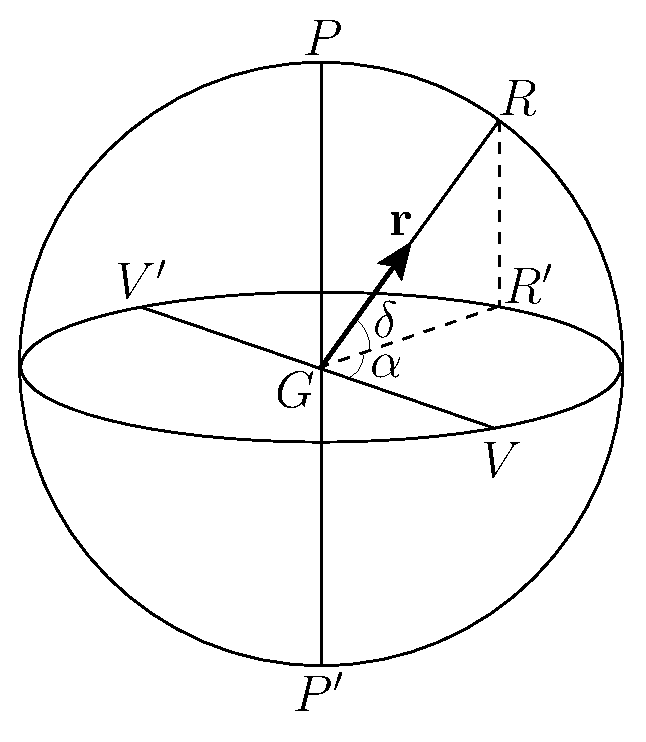
\includegraphics[height=3in]{epsfiles/sphere2.eps}}
\caption{Celestial coordinates. Here, $G$ is the Earth, $R$  a celestial object, and $R'$ the object's 
projection onto the plane of the celestial equator, $VR'V'$.}\label{f2}
\end{figure}

Let $G$ be the Earth. Consider a general celestial object, $R$. See Figure~\ref{f2}. The location of $R$ on the celestial sphere
is conveniently specified by  two angular coordinates, $\delta$ and $\alpha$. Let $GR'$ be the
projection of $GR$ onto the equatorial plane. The coordinate $\delta$, which is known as  {\em declination}, is  the angle subtended between $GR'$ and $GR$. Objects north of the celestial equator have positive
declinations, and vice versa. It follows that objects on the celestial equator have declinations of $0^\circ$,
whereas the north and south celestial poles have declinations of $+90^\circ$ and $-90^\circ$, respectively.
The coordinate $\alpha$, which is known as  {\em right ascension}, is the angle subtended between 
$GV$ and $GR'$. Right ascension increases from west to east (that is, in the opposite direction to the
celestial sphere's diurnal rotation). Thus, the vernal and autumnal equinoxes have right ascensions of $0^\circ$ and $180^\circ$, respectively. Note that $\alpha$ lies in the range $0^\circ$ to
$360^\circ$. Right ascension is sometimes measured in hours, instead of degrees, with one hour corresponding to
$15^\circ$ (because it takes 24 (sidereal) hours for the celestial sphere to complete
one diurnal rotation). In this scheme, the vernal and autumnal equinoxes
have right ascensions of 0 hours and 12 hours, respectively. Moreover, $\alpha$ lies in the
range 0  to 24 hours. (Incidentally, in this treatise, $\alpha$ is measured
relative to the mean equinox at date, unless otherwise specified.)
Finally, let ${\bf r}$ be a unit vector which is directed from the Earth to $R$. See Figure~\ref{f2}. It is easily
demonstrated that 
\begin{equation}\label{e1}
{\bf r} = \cos\delta\,\cos\alpha\,{\bf v} + 
\cos\delta\,\sin\alpha\,{\bf u} + \sin\delta\,{\bf p},
\end{equation}
and
\begin{align}\label{e2}
\sin\delta &= {\bf r}\cdot {\bf p},\\[0.5ex]
\tan\alpha &= \frac{{\bf r}\cdot{\bf u}}{{\bf r}\cdot {\bf v}}.\label{e3}
\end{align}

\section{Ecliptic Circle}
During the course of a year, the Sun's intrinsic motion causes it to trace out a fixed circle that bisects the celestial sphere. This circle is known as the {\em ecliptic}. The Sun travels around the ecliptic from west to east (that is, in the opposite direction
to the celestial sphere's diurnal rotation). Moreover, the ecliptic circle is inclined at a fixed angle of $\epsilon = 23^\circ 26'$ to the celestial equator.
This angle actually represents the fixed inclination of the Earth's axis of rotation to the normal to its orbital
plane.\footnote{In fact, $\epsilon$ is very slowly decreasing in time. The value of
$\epsilon$ used in  the Almagest is $23^\circ 51'$. However, the true value of $\epsilon$  in Ptolemy's day was $23^\circ 41'$.}

\begin{figure}
\centerline{\includegraphics[height=3in]{epsfiles/sphere3.eps}}
\caption{The ecliptic circle. Here, $P$, $P'$, $Q$, $Q'$, $V$, $V'$, $S$, 
and $S'$ denote the north celestial pole, the south celestial pole, the north ecliptic pole, the south
ecliptic pole, the vernal equinox, the autumnal equinox, the summer solstice, and the winter
solstice, respectively. Moreover, $VUV'U'$ is the celestial equator, $VSV'S'$ the ecliptic, and $PP'$ the
celestial axis.}\label{f3}
\end{figure}

The vernal equinox, $V$, is defined as the point at which the ecliptic crosses the celestial equator
from south to north (in the direction of the Sun's ecliptic motion). See Figure~\ref{f3}. Likewise, the autumnal equinox, $V'$, is the point at which the ecliptic crosses the
celestial equator from north to south.  In addition, the {\em summer solstice}, $S$, is the
point on the ecliptic that is furthest north of the celestial equator, whereas the
{\em winter solstice}, $S'$, is the  point that is furthest south. It follows that the lines $VV'$ and $SS'$
are perpendicular. Let $QQ'$ be the normal to the plane of the ecliptic that passes through the Earth, as shown in Figure~\ref{f3}.  
Here, $Q$ is termed the {\em northern ecliptic pole}, and $Q'$ the {\em southern ecliptic pole}. 
It is easily demonstrated that
\begin{align}
{\bf s} &= \cos\epsilon\,{\bf u}+ \sin\epsilon\,{\bf p},\label{e4}\\[0.5ex]
{\bf q} &= -\sin \epsilon\,{\bf u} + \cos\epsilon\,{\bf p},\label{e5}
\end{align}
where ${\bf s}$ is a unit vector that is directed from the Earth to the summer solstice, and ${\bf q}$ a unit vector that is directed from the Earth to the north ecliptic pole. See Figure~\ref{f3}. We can also write
\begin{align}
{\bf u} &= \cos\epsilon\,{\bf s} - \sin\epsilon\,{\bf q},\label{e4p}\\[0.5ex]
{\bf p} &= \sin\epsilon\,{\bf s} + \cos\epsilon\,{\bf q}.\label{e5p}
\end{align}
Thus, ${\bf v}$, ${\bf s}$, and ${\bf q}$ constitute another right-handed, mutually perpendicular, set of unit vectors. 

\begin{figure}
\centerline{\includegraphics[height=3in]{epsfiles/sphere4.eps}}
\caption{Ecliptic coordinates. Here, $G$ is the Earth, $R$ a celestial
object, and $R'$ the object's  projection onto the ecliptic plane, $VR'V'$.}\label{f4}
\end{figure}

\section{Ecliptic Coordinates}
It is convenient to specify the positions of the Sun, Moon, and planets in the sky using
a pair of angular coordinates, $\beta$ and $\lambda$, that are measured with respect to the
ecliptic, rather than the celestial equator. Let $G$ and $R$ denote the Earth and  a celestial object, respectively, and let $GR'$ denote the
projection of the line $GR$ onto the plane of the ecliptic, $VR'V'$. See Figure~\ref{f4}. The coordinate $\beta$, which
is known as {\em ecliptic latitude}, is the angle subtended between $GR'$ and $GR$. Objects north
of the ecliptic plane have positive ecliptic latitudes, and vice versa. The coordinate $\lambda$,
which is known as {\em ecliptic longitude}, is the angle subtended between $GV$ and
$GR'$. Ecliptic longitude increases from west to east (that is, in the same direction that the Sun travels
around the ecliptic). (Again, in this treatise, $\lambda$ is measured relative
to the mean equinox at date, unless specified otherwise.)
Note that the basis vectors in the ecliptic coordinate system are
${\bf v}$, ${\bf s}$, and ${\bf q}$, whereas the corresponding basis vectors in the
celestial coordinate system are
${\bf v}$, ${\bf u}$, and ${\bf p}$. See Figures~\ref{f1} and \ref{f3}. By analogy with Equations~(\ref{e1})--(\ref{e3}), we can write
\begin{align}%\label{e8w}
{\bf r} &= \cos\beta\,\cos\lambda\,{\bf v} + \cos\beta\,\sin\lambda\,{\bf s} +\sin\beta\,{\bf q},\label{e1p}\\[0.5ex]
\sin\beta &= {\bf r}\cdot {\bf q},\\[0.5ex]
\tan\lambda &= \frac{{\bf r}\cdot{\bf s}}{{\bf r}\cdot {\bf v}},
\end{align}
where ${\bf r}$ is a unit vector that is directed from $G$ to $R$. 
Hence, it follows from Equations~(\ref{e1}), (\ref{e4}), and (\ref{e5}) that
\begin{align}
\sin\beta &= \cos\epsilon\,\sin\delta - \sin\epsilon\,\cos\delta\,\sin\alpha,\\[0.5ex]
\tan\lambda &= \frac{\cos\epsilon\,\cos\delta\,\sin\alpha+\sin\epsilon\,\sin\delta}{\cos\delta\,\cos\alpha}.
\end{align}
These expressions specify the transformation from celestial to ecliptic
coordinates. The inverse transformation follows from Equations~(\ref{e2}), (\ref{e3}), and (\ref{e4p})--(\ref{e1p}):
\begin{align}\label{e10}
\sin\delta &= \cos\epsilon\,\sin\beta +\sin\epsilon\,\cos\beta\,\sin\lambda,\\[0.5ex]
\tan\alpha&=  \frac{\cos\epsilon\,\cos\beta\,\sin\lambda-\sin\epsilon\,\sin\beta }{\cos\beta\,\cos\lambda}.\label{e11}
\end{align}

Figures~\ref{map1} and \ref{map2} show all stars of visible magnitude less than $+6$ lying
within $15^\circ$ of the ecliptic. Table~\ref{tstar} gives the ecliptic longitudes (relative to the start of the appropriate zodiacal sign; see next section), ecliptic latitudes, and
visible magnitudes of a selection
of these stars that lie within $10^\circ$ of the ecliptic. The figures and the table can
be used 
 to convert ecliptic longitude and latitude into approximate position
in the sky against the backdrop of the fixed stars.

Figures~\ref{map1} and \ref{map2}  and   Table~\ref{tstar}  contain more or less the same information  as that contained in Section~5 of Book VII of the Almagest
(although we have restricted our attention to stars that lie relatively close to the ecliptic). Incidentally, the ancient Greeks did not individually name stars, describing them instead 
in figurative terms, such as ``the bright, reddish star on the right shoulder of Orion" (Betelgeuse). 

\section{Signs of the Zodiac}\label{szod}
The {\em signs of the zodiac}  are a well-known set of names given
to $30^\circ$ long segments of the ecliptic circle. Thus, the sign of Aries extends
over the range of ecliptic longitudes $0^\circ$--$30^\circ$, the sign of Taurus
over the range $30^\circ$--$60^\circ$, and so on. Note that, as
a consequence of the precession of the equinoxes, the signs
of the zodiac no longer coincide with the constellations of the same name. 
See Figures~\ref{map1} and \ref{map2}. (Incidentally, Ptolemy was well aware of this fact because, even in his day, the signs of the zodiac did not coincide with the constellations. The signs coincided with the constellations in the time of the ancient Mesopotamians; that is, about 1500 BC.)
The 12 zodiacal signs are listed in the following table.  It can be seen from the table that ecliptic longitude $72^\circ$ corresponds to the
twelfth degree of Gemini, and ecliptic longitude $242^\circ$  to the second degree of
Sagittarius, et cetera.
\begin{table}[h]
\centering
\begin{tabular}{lcl|lcl|lcl}
Sign & Abbr.\ & Longitude & Sign & Abbr.\ &Longitude & Sign & Abbr.\ &  Longitude\\[-0.0ex]\hline
&&&&&&&&\\[-1.8ex]
Aries & AR & $000^\circ$--$030^\circ$ & Leo & LE & $120^\circ$--$150^\circ$&Sagittarius & SG & $240^\circ$--$270^\circ$\\
Taurus & TA & $030^\circ$--$060^\circ$ & Virgo & VI & $150^\circ$--$180^\circ$ & Capricorn & CP & $270^\circ$--$300^\circ$\\
Gemini & GE & $060^\circ$--$090^\circ$ & Libra & LI & $180^\circ$--$210^\circ$ & Aquarius & AQ & $300^\circ$--$330^\circ$\\
Cancer & CN & $090^\circ$--$120^\circ$ & Scorpio & SC & $210^\circ$--$240^\circ$ & Pisces & PI & $330^\circ$--$360^\circ$\\
\end{tabular}
\end{table}

Incidentally, the term zodiac comes from the Greek ζῳδιακός κύκλος, meaning ``circle of little animals".  The Greek names for the
zodiacal signs were  Κριός (Ram),  Ταῦρος (Bull), Δίδυμοι (Twins), Κάρκινος (Crab), 
Λέων (Lion), Παρθένος (Virgin), Ζυγός (Balance/scale), Σκορπιός (Scorpion),
Τοξότης (Archer), Αἰγόκερως (Goat-horned), Ὑδροχόος (Water-pourer), and  Ἰχθύες  (Fishes). The familiar names listed in the previous table are
merely latinized versions of the Greek names. 

\section{Ecliptic Declinations and Right Ascensions.}
According to Equations~(\ref{e10}) and (\ref{e11}), the celestial coordinates of a point on the ecliptic circle (which corresponds to $\beta = 0$) that has ecliptic
longitude $\lambda$ are specified by
\begin{align}\label{e15q}
\sin \delta &= \sin\epsilon\,\sin\lambda,\\[0.5ex]
\tan\alpha&=  \cos\epsilon\,\tan\lambda.\label{e15r}
\end{align}
The previous formulae have been used to construct
Tables~\ref{tec1} and \ref{tec2}, which  list the declinations and right ascensions of a set of equally spaced points on the ecliptic circle.
Note that $\lambda$ is measured relative to the start of the appropriate zodiacal sign. 

 Tables ~\ref{tec1} and \ref{tec2}  contain essentially the same information
as is contained in the ``Table of inclinations" (Κανόνιoν λοξώσεως) that appears in Section~15 of Book~I of the Almagest. The slight difference between the entries appearing in our
tables  and those appearing in Ptolemy's table is due to the fact that Ptolemy adopted the value $23^\circ 51' 20''$ for the obliquity of the ecliptic, whereas we
are using the modern (and correct) value $23^\circ26'$. 

\section{Local Horizon and Meridian}
Consider a general observation site $X$ located on the surface of the Earth. (Note that, in the following, it is
tacitly assumed that the site lies the Earth's northern hemisphere. However, the analysis also
applies to sites situated in the the southern hemisphere.)
The local {\em zenith}, $Z$, is the point on the celestial sphere that is directly overhead at $X$,
whereas the {\em nadir}, $Z'$,  is the point that is directly underfoot. See Figure~\ref{f5}. The {\em horizon}\/
is the tangent plane to the Earth at $X$, and divides the celestial sphere into two  halves. The upper half,
containing the zenith, is visible from site $X$, whereas the lower half is invisible. 

\begin{figure}
\centerline{\includegraphics[height=3in]{epsfiles/sphere5.eps}}
\caption{A general observation site $X$, of latitude $L$,  on the surface of the Earth. Here, $P$, $P'$, $Z$, and $Z'$
denote the directions to the north celestial pole, south celestial pole, zenith, and nadir, respectively. The line
$NS$ represents the local horizon.}\label{f5}
\end{figure}

\begin{figure}
\centerline{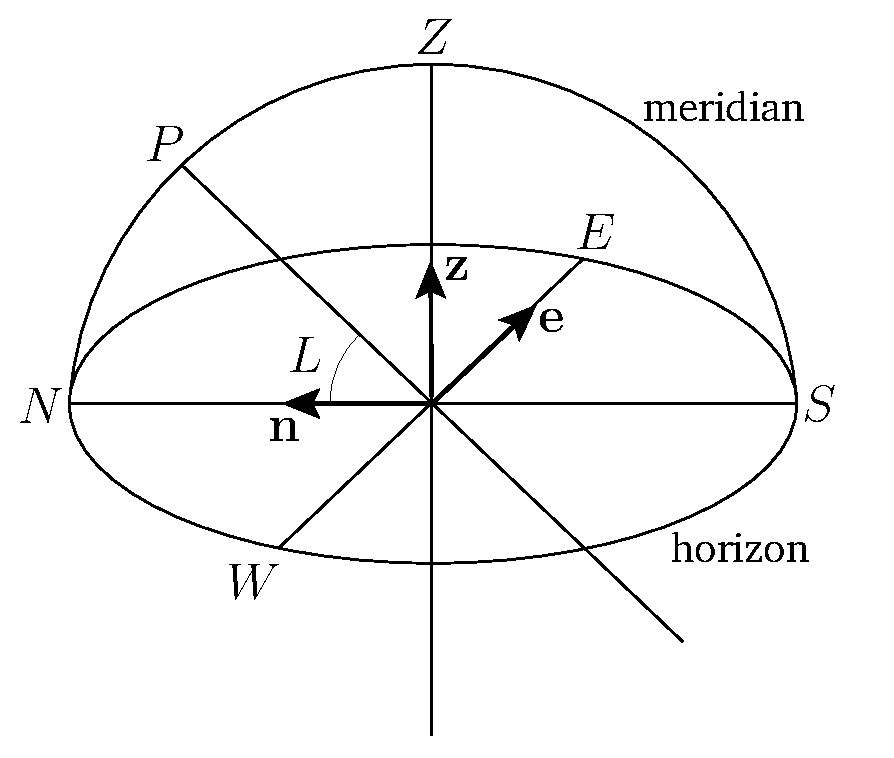
\includegraphics[height=3in]{epsfiles/sphere6.eps}}
\caption{The local horizon and meridian. Here, $N$, $S$, $E$, $W$
denote the north. south, east, and west compass points, $Z$ the
zenith, and $P$ the north celestial pole. Moreover, $NESW$ is the horizon, and
$NPZS$ the meridian.}\label{f6}
\end{figure}

Figure~\ref{f6} shows the visible half of the celestial sphere at observation site $X$. 
Here, $NESW$ is the local horizon, and  $N$, $E$, $S$, and $W$ are
the north, east, south, and west compass points, respectively. The plane $NPZS$,
which passes through the north and south compass points, as well as the zenith,
is known as the local {\em meridian}. The meridian is perpendicular
to the horizon. The north celestial pole lies in the meridian plane, and
is elevated an angular distance $L$ above the north compass point. See Figures~\ref{f5} and \ref{f6}. Here,
$L$ is the terrestrial {\em latitude}\/ of observation site $X$. It is helpful to
define three, right-handed, mutually perpendicular,  local unit vectors; ${\bf e}$, ${\bf n}$, and ${\bf z}$.
Here, 
${\bf e}$ is directed toward the east compass point, ${\bf n}$ toward the north compass point, and ${\bf z}$  toward the zenith. See Figures~\ref{f6}. 

\begin{figure}
\centerline{\includegraphics[height=3in]{epsfiles/sphere8.eps}}
\caption{The local meridian.}\label{f7}
\end{figure}

Figure~\ref{f7} shows the meridian plane at $X$. Let the line $MM'$ lie
in this plane such that it is perpendicular to the celestial axis, $PP'$. Moreover, let
$M$ lie in the visible hemisphere. It is helpful to define the unit vector ${\bf m}$ which
is directed toward $M$, as shown in the diagram. It is easily seen that
\begin{align}\label{e14}
{\bf n} &= \cos L\,{\bf p} - \sin L\,{\bf m},\\[0.5ex]
{\bf z} &= \sin L\,{\bf p} + \cos L\,{\bf m}.\label{e15}
\end{align}

\begin{figure}
\centerline{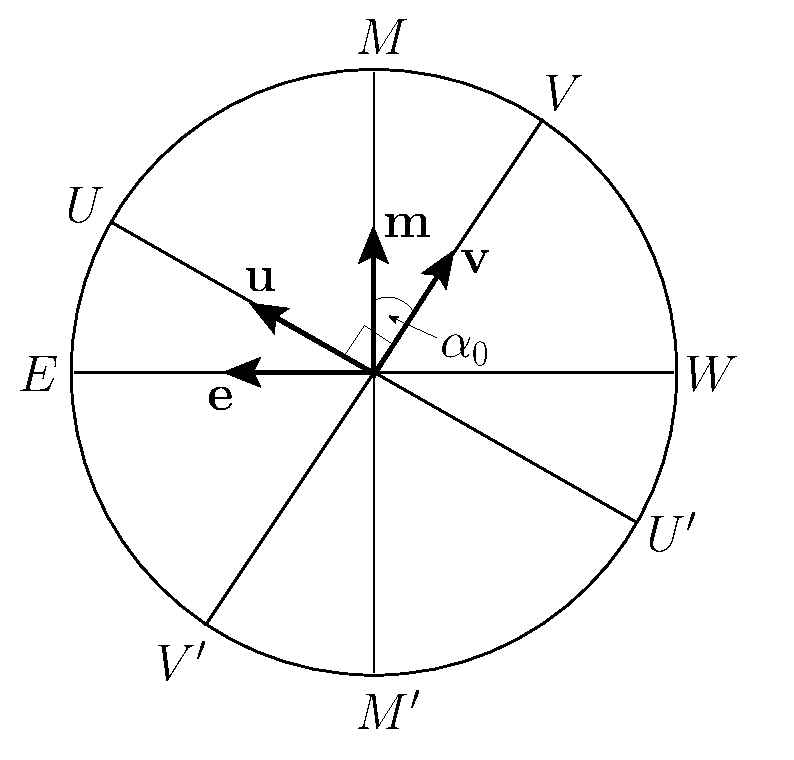
\includegraphics[height=3in]{epsfiles/sphere9.eps}}
\caption{The local celestial equator.}\label{f8}
\end{figure}

Figure~\ref{f8} shows the celestial equator viewed from observation site $X$. Here, $\alpha_0$ is
the right ascension of the celestial objects culminating (that is, attaining 
their highest altitude in the sky) on the meridian at the time of observation. Incidentally, it is
easily demonstrated that all objects culminating on the meridian at
any instant in time have the  same right ascension. Note that the angle $\alpha_0$
increases uniformly in time, at the rate of $15^\circ$ a (sidereal) hour, due to the diurnal motion of the celestial
sphere. It can be seen from the diagram that
\begin{align}
{\bf m} &= \sin \alpha_0\,{\bf u} + \cos \alpha_0\,{\bf v},\\[0.5ex]
{\bf e} &=\cos \alpha_0 \,{\bf u} -\sin \alpha_0\,{\bf v}.\label{e17}
\end{align}
Thus, from Equations~(\ref{e14}) and (\ref{e15}),
\begin{align}
{\bf e} &= -\sin \alpha_0\,{\bf v} + \cos \alpha_0\,{\bf u},\\[0.5ex]
{\bf n} &= -\sin L\,\cos \alpha_0\,{\bf v} - \sin L\,\sin \alpha_0\,{\bf u} + \cos L\,{\bf p},\label{xx}\\[0.5ex]
{\bf z} &= \cos L\,\cos \alpha_0\,{\bf v} + \cos L\,\sin \alpha_0\,{\bf u} + \sin L\,{\bf p}.\label{zz}
\end{align}
Similarly, from Equations~(\ref{e4p}) and (\ref{e5p}),
\begin{align}
{\bf e}&= -\sin \alpha_0\,{\bf v} + \cos\epsilon\,\cos \alpha_0\,{\bf s} - \sin\epsilon\,\cos \alpha_0\,{\bf q},\label{e25w}\\[0.5ex]
{\bf n} &= -\sin L\,\cos \alpha_0\,{\bf v} + (\cos L\,\sin \epsilon-\sin L\,\cos \epsilon\,\sin \alpha_0)\,{\bf s} + (\cos L\,\cos \epsilon+\sin L\,\sin \epsilon\,\sin \alpha_0)\,{\bf q},\label{e24w}\\[0.5ex]
{\bf z} &= \cos L\,\cos \alpha_0\,{\bf v} + (\sin L\,\sin\epsilon + \cos L\,\cos\epsilon\,\sin \alpha_0)\,{\bf s} + (\sin L\,\cos\epsilon-\cos L\,\sin\epsilon\,\sin \alpha_0)\,{\bf q}.\label{e26w}
\end{align}

\section{Horizontal Coordinates}
It is convenient to specify the positions of celestial objects  in the sky, when viewed from
a particular observation site, $X$, on the Earth's surface, using a pair of angular coordinates, $a$ and $A$,
that are measured with respect to the local horizon. Let $R$ denote
a celestial object, and $XR'$ the projection of the line $XR$ onto the
horizontal plane, $NESW$. See Figure~\ref{f9}. The coordinate $a$, which
is known as {\em altitude}, is the angle subtended between $XR'$ and
$XR$. Objects above the horizon have positive altitudes, whereas
objects below the horizon have negative altitudes. The
zenith has altitude $90^\circ$, and the horizon altitude $0^\circ$. The coordinate $A$,
which is known as {\em azimuth}, is the angle subtended between 
$XN$ and $XR'$. Azimuth increases from the north towards the east. Thus, the
north, east, south, and west compass points have azimuths of
$0^\circ$, $90^\circ$, $180^\circ$, and $270^\circ$, respectively. 
Note that the basis vectors in the horizontal coordinate system are ${\bf e}$,
${\bf n}$, and ${\bf z}$, whereas the corresponding basis vectors in the
celestial coordinate system are ${\bf v}$, ${\bf u}$, and ${\bf p}$. See Figures~\ref{f1} and \ref{f6}. By analogy with Equations~(\ref{e1})--(\ref{e3}), we can write
\begin{align}\label{e27}
{\bf r} &= \cos a\,\sin A\,{\bf e} + \cos a\,\cos A\,{\bf n}  + \sin a\,{\bf z},\\[0.5ex]
\sin a &= {\bf r}\cdot {\bf z},\\[0.5ex]
\tan A &= \frac{{\bf r}\cdot {\bf e}}{{\bf r}\cdot {\bf n}},
\end{align}
where ${\bf r}$ is a unit vector directed from $X$ to $R$.
Hence, it follows from Equations~(\ref{e1}), and (\ref{xx})--(\ref{zz}), that
\begin{align}\label{e30}
\sin a &= \sin L\,\sin \delta + \cos L\,\cos \delta\,\cos(\alpha-\alpha_0),\\[0.5ex]
\tan A &= \frac{\cos \delta\,\sin (\alpha-\alpha_0)}{\cos L\,\sin \delta - \sin L\,\cos\delta\,\cos(\alpha - \alpha_0)}.\label{e31}
\end{align}
These expressions allow us to calculate the altitude and azimuth of a
celestial object of declination $\delta$ and right ascension $\alpha$
that is viewed from an observation  site on the Earth's surface of terrestrial latitude $L$ at an instance in time when celestial objects of
right ascension $\alpha_0$ are culminating at the meridian..
According to Equations~(\ref{e1p}), and (\ref{e24w})--(\ref{e26w}), 
the altitude and azimuth of a similarly viewed point on the ecliptic (which corresponds to $\beta=0$) of ecliptic
longitude $\lambda$ are given by
\begin{align}\label{e32}
\sin a &= \cos L\,\cos\lambda\,\cos \alpha_0+ \sin L\,\sin\epsilon\,\sin \lambda
+ \cos L\,\cos\epsilon\,\sin\lambda\,\sin \alpha_0,\\[0.5ex]
\tan A &= \frac{\cos\epsilon\,\sin\lambda\,\cos \alpha_0-\cos\lambda\,\sin \alpha_0}
{\cos L\,\sin\epsilon\,\sin \lambda - \sin L\,\cos\lambda\,\cos \alpha_0-\sin L\,\cos\epsilon\,\sin\lambda\,\sin \alpha_0}.\label{e33}
\end{align}

\begin{figure}
\centerline{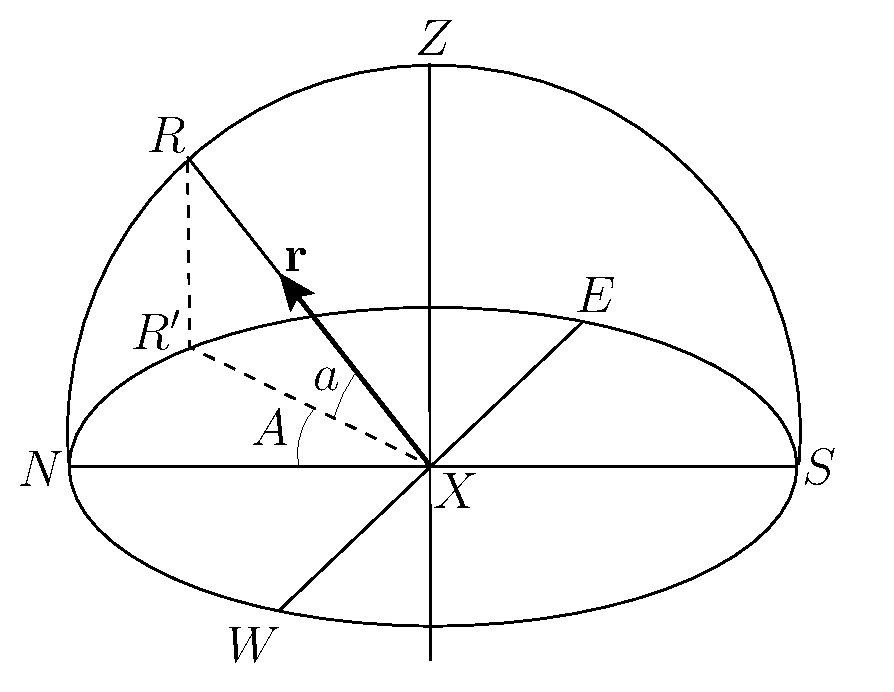
\includegraphics[height=3in]{epsfiles/sphere7.eps}}
\caption{Horizontal coordinates. Here, $R$ is a celestial object, and
$R'$ its projection onto the horizontal plane, $NESW$.}\label{f9}
\end{figure}

\section{Meridian Transits}
Consider a celestial object, of declination $\delta$ and right ascension $\alpha$, that is viewed from an
observation site on the Earth's surface of terrestrial latitude $L$. According to Equation~(\ref{e30}), the object culminates, or attains its highest
altitude in the sky, when $\alpha_0=\alpha$. This event is known as an {\em upper transit}. 
Furthermore, the object attains its lowest altitude in the sky when $\alpha_0=180^\circ + \alpha$.
This event is known as a {\em lower transit}. Both upper and lower
transits take place as the object in question passes through the meridian plane.

According to Equation~(\ref{e30}), the altitude of a celestial object at its upper
transit satisfies $\sin a_{\rm +} = \cos (L-\delta)$, implying that
\begin{equation}\label{e34}
a_{\rm +} = 90^\circ - |L-\delta|.
\end{equation}
Likewise, the altitude at its lower transit satisfies
$\sin a_{\rm -} =- \cos (L+\delta)$, giving
\begin{equation}\label{e35}
a_{\rm -} = |L+\delta| - 90^\circ.
\end{equation}
The previous two expressions allow us to group celestial objects into
three classes. Objects with declinations
satisfying $|L+\delta|> 90^\circ$  never set; that is, their
lower transits lie above the horizon. Objects with declinations
satisfying $|L-\delta|>90^\circ$  never rise; that is,
their upper transits lie below the horizon. Finally, objects with
declinations that satisfy neither of the two previous inequalities
both  rise and set  during the course of a day. It follows that all celestial objects appear to rise and set  when viewed from an observation  site on the
terrestrial equator (which corresponds to $L=0^\circ$) . On the other hand, when viewed from an observation site at the north pole (which corresponds to  $L=90^\circ$),
objects north of the celestial equator never set, while objects south of the
celestial equator never rise, and  vice versa  for objects viewed from the south pole.  All three classes of
celestial object are present when the sky is viewed  from an observation site on the Earth's surface of intermediate latitude.

\section{Principal Terrestrial Latitude Circles}
According to Equation~(\ref{e15q}),  the Sun's
declination varies between $-\epsilon$ and $+\epsilon$ during the course of
a year. 
It follows from Equation~(\ref{e34}) that it is only possible for the  Sun to have an
upper transit at the
zenith  in a region of the Earth whose
latitude lies between $-\epsilon$
and $\epsilon$. The  circles of latitude bounding this region are known
as the {\em tropics}. Thus, the {\em tropic of Capricorn}---so-called
because the Sun is at the winter solstice, and, therefore, at the
first point of Capricorn (that is, the zeroth degree of Capricorn), when  it culminates at the
zenith at this latitude---lies at  $L=-23^\circ 26'$. Moreover,
the {\em tropic of Cancer}---so-called
because the Sun is at the summer solstice, and, therefore, at the
first point of Cancer, when  it culminates at the
zenith at this latitude---lies at $L=+23^\circ 26'$. 

Equations (\ref{e34}) and (\ref{e35}) imply that the Sun
does not rise for part of the year, and does not set for part of the year, 
in two regions of the Earth whose terrestrial latitudes satisfy $|L|> 90^\circ - \epsilon$.
These two regions are bounded by the  poles and two circles of latitude
 known as the {\em arctic circles}. The
{\em south arctic circle}\/ lies at  $L=-66^\circ 34'$. Likewise,
the {\em north arctic circle}\/ lies at  $L=+66^\circ 34'$.  Incidentally, the word ``arctic'' comes from the Greek ἀρκτικός, meaning ``of the bear", and is so called because the most prominent
northern constellations are the ``great bear" and the  ``little bear". 

The equator, the two tropics, and the two arctic circles constitute the
five {\em principal latitude circles}\/ of the Earth, and are shown in Figure~\ref{f10}.

\begin{figure}
\centerline{\includegraphics[height=3in]{epsfiles/sphere10.eps}}
\caption{The principal latitude circles of the Earth.}\label{f10}
\end{figure}

\section{Equinoxes and Solstices}
The ecliptic longitude of the Sun when it reaches the vernal equinox is $\lambda = 0^\circ$.
It follows, from Equation~(\ref{e32}), that the altitude of the Sun on the
day of the equinox is given by $\sin a = \cos L\,\cos \alpha_0$. Thus, the Sun rises
when $\alpha_0=-90^\circ$, culminates at an altitude of $90^\circ - |L|$ when $\alpha_0 = 0^\circ$, and sets when
$\alpha_0=90^\circ$. We conclude that the length of the equinoctial day is $180$ time-degrees, which
is equivalent to 12 hours (because $15^\circ$ of right ascension cross the
meridian in one hour). 
Thus, day and night are equally long on the day of the vernal equinox.  (The word equinox is derived from the Latin word {\em aequinoctium}, which means ``equal night".) It is easily
demonstrated that the same is true on the day of the autumnal equinox. 

The ecliptic longitude of the Sun when it reaches the summer solstice is
$\lambda = 90^\circ$. It follows that the altitude of the Sun on the day of the
solstice is given by $\sin a = \sin L\,\sin \epsilon + \cos L\,\cos\epsilon\,\sin \alpha_0$.
Thus, the Sun rises when $\alpha_0=-\sin^{-1}(\tan L\,\tan\epsilon)$, 
culminates at an altitude of $90^\circ - |L- \epsilon|$ when $\alpha_0=90^\circ$, and sets when $\alpha_0=180^\circ + \sin ^{-1}(\tan L\,\tan\epsilon)$. We conclude that the length  of the longest day of the year in the Earth's northern hemisphere
(which, of course, occurs when the Sun reaches the summer solstice)
is $180^\circ +2\,\sin ^{-1}(\tan L\,\tan\epsilon)$ time-degrees. Likewise, the
length of the shortest night (which also occurs at the summer solstice) is $180-2\, \sin^{-1}(\tan L\,\tan\epsilon)$ time-degrees.
These formulae are only valid for northern latitudes below the arctic circle. 
At higher latitudes, the Sun never sets for part of the year, and the longest
``day" is consequently longer than 24 hours. It is easily
demonstrated that the shortest day in the Earth's northern hemisphere, which takes place when the Sun
reaches the winter solstice, is equal to the shortest night, and the longest
night (which also occurs at the winter solstice) to the longest day. Moreover, the Sun
culminates at an altitude of $90^\circ - |L + \epsilon|$  on day of the winter solstice. 
Again, at latitudes above the arctic circle,
the Sun never rises for part of the year, and the longest ``night" is
consequently longer than 24 hours. 

Consider an observation  site on the Earth's surface of latitude $L$ that lies
above the northern arctic circle. The declination of the Sun on the
first day after the spring equinox on which it fails to set is $\delta = 90^\circ - L$. According
to Equation~(\ref{e15q}), the Sun's ecliptic longitude on this day is $\sin ^{-1} (\cos L/\sin \epsilon)$.
Likewise, the declination of the Sun on the day  when it starts to  set again
is $\delta = 90^\circ - L$, and its ecliptic longitude is $180^\circ -
\sin^{-1}(\cos L/\sin \epsilon)$. Assuming that the Sun
travels around the ecliptic circle at a uniform rate (which is approximately
true), the fraction of a year that the Sun stays above the horizon
in summer is $0.5-\sin^{-1}(\cos L/\sin \epsilon)/180^\circ$. It is easily
demonstrated that the fraction of a year that the Sun stays
below the horizon in winter is also  $0.5-\sin^{-1}(\cos L/\sin \epsilon)/180^\circ$.

\section{Terrestrial Climes}
Table~\ref{t3} specifies the length of the longest day, as well as the altitude of the
Sun when it culminates at the meridian on the days of the equinoxes and solstices, calculated for a set of observation sites in the northern hemisphere with equally
spaced terrestrial latitudes. This table was constructed
using the formulae in the previous section.  The table can be adapted to observation sites in the Earth's
southern hemisphere via the following simple transformation: $L\rightarrow -L$, Summer $\leftrightarrow$ Winter, N $\leftrightarrow$ S. For instance, at a latitude of $-10^\circ$, the longest day, which corresponds
to the winter solstice, is of length $12^h35^m$. Moreover, on this day, the Sun's upper transit
is  south  of the zenith, at an altitude of $+76^\circ 34'$. 

Table~\ref{t3} contains essentially the same information as is contained in the discussion that appears in Section~6 of Book~II of the Almagest. 

\section{Ecliptic Ascensions}
Consider the rising, or {\em ascension}, of celestial objects at the eastern
horizon, as viewed from a particular observation site on the Earth's
surface. If the observation site lies on the terrestrial equator then all
celestial objects appear to ascend at right angles to the horizon. This process is
known as {\em right ascension}. On the other hand, if the
observation site does not lie at the equator then celestial objects
appear to ascend at an oblique angle to the horizon. This process is known
as {\em oblique ascension}. For the case of right ascension, it is
easily demonstrated that all celestial objects with the same celestial
longitude ascend simultaneously. Indeed, celestial longitude is generally
known as ``right ascension'' because, in the case of right ascension, the
celestial longitude of an object (in hours) is simply the time elapsed between the ascension of the vernal equinox, and the ascension of the object
in question.

Let us now consider the ascension of points on the ecliptic.
Applying Equation~(\ref{e30}) to a point on the celestial equator (which corresponds to $\delta=0$)
of right ascension $\alpha$, we obtain
\begin{equation}
\sin a = \cos L\,\cos(\alpha - \alpha_0) = \cos L\,\sin (\alpha_0-\alpha + 90^\circ).
\end{equation}
It follows that we can write
\begin{equation}
\alpha_0 = \alpha-90^\circ,
\end{equation}
where $\alpha$ is the right ascension of the point on the celestial equator that 
ascends at the eastern horizon (that is, $a=0$ and $da/dt>0$) at the same time that celestial objects of right ascension $\alpha_0$ are culminating at
the meridian. Substituting this result into Equation~(\ref{e32}), 
we get
\begin{equation}
\sin a= \cos L\,\cos\lambda\,\sin\alpha + \sin L\,\sin\epsilon\,\sin\lambda - \cos L\,\cos\epsilon\,\sin\lambda\,\cos\alpha,
\end{equation}
which implies that if $a=0$ and $da/dt>0$ then
\begin{equation}\label{e39}
\tan \lambda = \frac{\cos L\,\sin \alpha}{\cos L\,\cos\epsilon\,\cos\alpha-\sin\epsilon\,\sin L}.
\end{equation}
This expression 
specifies the ecliptic longitude, $\lambda$, of the point on the ecliptic circle that 
ascends simultaneously with a point on the celestial equator of right ascension $\alpha$. 
Note, incidentally, that points on the celestial equator  ascend at a  uniform rate of $15^\circ$ an hour at all viewing sites on the Earth's
surface (except the poles, where the celestial equator does not ascend at all). The same is not true of points on the ecliptic. Expression (\ref{e39})
can be inverted to give
\begin{equation}\label{e40}
\alpha = \tan^{-1}(\tan \lambda\,\cos \epsilon) - \sin^{-1}\left[
\frac{\sin \lambda\,\sin \epsilon\,\tan L}{(1-\sin^2\lambda\,\sin^2\epsilon)^{1/2}}\right].
\end{equation}

The solution of Equation~(\ref{e40}) for observation sites lying above
the arctic circle is complicated by the fact that, at such sites, a section of the ecliptic never
sets, or descends,  and a section never ascends. It is easily demonstrated that the
section that never descends lies between ecliptic longitudes
$\lambda_c$ and $180^\circ-\lambda_c$, whereas the section that 
never ascends lies between longitudes $180^\circ+\lambda_c$ and
$360^\circ-\lambda_c$. Here, $\lambda_c=\sin^{-1}(\cos L/\sin\epsilon)$. 
Points on the ecliptic of longitude $\lambda_c$, $180^\circ-\lambda_c$,
$180^\circ+\lambda_c$, and $360^\circ-\lambda_c$ ascend simultaneously
with points on the celestial equator of right ascension
$360^\circ - \alpha_c$, $\alpha_c$, $360^\circ-\alpha_c$, and $\alpha_c$,
respectively. Here, $\alpha_c=\cos^{-1}(1/\tan L\,\tan\epsilon)$. 

Tables~\ref{tx}--\ref{ty} list the ascensions of a series of equally spaced points on the ecliptic
circle, as viewed from a set of observation sites in the Earth's northern
hemisphere with different terrestrial latitudes. The tables were calculated with the aid of
formula (\ref{e40}). Let us now illustrate the use of these tables.

Consider a day on which the Sun is at ecliptic longitude 14LE00 (that is, 
$14^\circ 00'$ into the sign of Leo). What is the length of the day (that is, the period between sunrise and sunset) at
an observation site on the Earth's surface of latitude $+30^\circ$? Consulting
Table~\ref{tz}, we find that the Sun ascends simultaneously with a
point on the celestial equator of right ascension $126^\circ 32'$. Now,
the ecliptic is a great circle on the celestial sphere. Hence, exactly half of the ecliptic
is  visible from any observation site on the Earth's surface. This implies that
when a given point on the ecliptic circle is ascending, the point directly
opposite it on the circle is descending, and vice versa. Let us
term the directly opposite point the {\em complementary point}. 
By definition, the difference in ecliptic longitude between a given point on the
ecliptic circle and its complementary point is $180^\circ$. Thus, the
complementary point to 14LE00 is 14AQ00. It follows that
 14AQ00 ascends at the same time that 14LE00 descends.
 In other words, the Sun sets when 14AQ00 ascends.
 Consulting Table~\ref{tz}, we find that the Sun sets at the
 same time that a point on the celestial equator of right ascension 
 $326^\circ 23'$ rises. Thus, in the time interval between the rising and
 setting  of the Sun, a $326^\circ23'-126^\circ 32' = 199^\circ 51'$ section
 of the celestial equator ascends at the eastern horizon. However, points on the celestial
 equator ascend at the uniform rate of $15^\circ$ an hour. Thus,
 the length, in hours,  of the period between the rising and setting of the Sun  is $199^\circ 51'/15^\circ = 13^h 19^m.$ In other words, the
 length of the day in question is $13^h 19^m$.
 
 The previous calculation is slightly inaccurate for a number of reasons. Firstly, it neglects the
 fact that the Sun is continuously  moving  on the ecliptic circle at the rate of about $1^\circ$ a day.
 Secondly, it neglects the fact that the celestial equator ascends
 at the rate of $15^\circ$ per  sidereal, rather than 
 solar, hour. A sidereal hour is $1/24$th of a {\em sidereal day},
 which is the time between successive upper transits  of a fixed celestial object, such as a star. On the other hand, a solar hour is $1/24$th of a
 {\em solar day}, which is the mean time between successive upper transits
 of the Sun. A sidereal day is shorter than a solar day by 4 minutes. 
 Fortunately, it turns out that these first two inaccuracies largely
 cancel one another out. Another source of inaccuracy is the fact that, due to
 refraction of light by the atmosphere, the Sun is actually $1^\circ$ below
 the horizon when it appears to rise or set. The final source of inaccuracy
 is the fact that the Sun has a finite angular extent (of about half a degree),
 and that, strictly speaking, dawn and dusk commence when the Sun's upper limb rises and sets, respectively. Of course, our calculation
 only deals  with the rising and setting of the center of the Sun. 
 Taken together, the previously mentioned inaccuracies can cause  the true length
 of a day differ from that calculated from the ascension tables by up
 to 15 minutes.
 
 Tables~\ref{tx}--\ref{ty} also effectively list the  descents of a series of equally spaced points on the ecliptic
circle, as viewed from a set of observation sites in the Earth's  southern 
hemisphere with different terrestrial latitudes (which are minus those specified in the various tables). For instance,
Table~\ref{tx1} gives the right ascensions of points on the celestial equator that  set simultaneously
with points on the ecliptic, as seen from an observation site at latitude $-10^\circ$. 

Consider a day on which the Sun is at ecliptic longitude 08SC00. Let us calculate the length of the day
at an observation site on the Earth's surface of latitude $-50^\circ$? Consulting Table~\ref{txx}, we find that
the Sun sets simultaneously with a point on the celestial equator of right ascension $233^\circ 09'$. Now,
the complementary point on the ecliptic to 08SC00 is 08TA00. Consulting Table~\ref{txx} again, we
find that this point sets simultaneously with a point on the celestial equator of
right ascension $18^\circ 07'$. It follows that the Sun rises simultaneously with the latter point. 
Thus, the time interval between the rising and setting of the Sun is $233^\circ 09'-18^\circ 07'=215^\circ 02'$
time-degrees, or $14^h 20^m$. 
 
 The {\em ascendent}, or  {\em horoscope}, is defined as the point on the ecliptic that is ascending at the eastern horizon.
 Suppose that we wish to find the  ascendent $2.6$ hours after 
 sunrise, as seen from an observation site of latitude $+55^\circ$, on a day
 on which the Sun has ecliptic longitude 16SC00. Of course, knowledge
 of the ascendent at the time of birth is key to drawing up a natal chart
 in astrology. Hence, this type of calculation was of great importance to the ancient Greeks. (It was of particular importance to Ptolemy, because he wrote the standard treatise on Greek natal
 astrology; the so-called {\em Tetrabiblos}.) 
 Consulting Table~\ref{tzz}, we find that, on the day in question, the Sun rises simultaneously with a point on the celestial equator of
 right ascension $248^\circ 46'$. Now, $2.6$ hours corresponds to
 $39^\circ00'$. Thus, the ascendent rises simultaneously with a point
 on the celestial equator of right ascension $248^\circ 46' + 39^\circ00'=
 287^\circ 46'$. Consulting Table~\ref{tzz} again, we find that, to the
 nearest degree, the ascendent at the time in question has ecliptic longitude 13SG00. 
 
Suppose, next, that we wish to find the right ascension, $\alpha$, of the point on the celestial equator
that culminates simultaneously with a given point on the ecliptic of
ecliptic longitude $\lambda$.
From Equation~(\ref{e33}), we can see that if $A=180^\circ$ then
$\tan A = 0$, and $\tan\lambda\,\cos \epsilon = \tan \alpha$, or
\begin{equation}
\alpha  = \tan ^{-1}(\tan \lambda\,\cos\epsilon).
\end{equation}
However, this expression is identical to expression (\ref{e40}),
when the latter is evaluated for the special case $L=0^\circ$. It follows
that our problem can be solved by consulting Table~\ref{tx}, which is the
ascension table for the case of right ascension. For instance, on a day on which the ecliptic
longitude of the Sun is 08TA00, we find from Table~\ref{tx} that
the right ascension of the point on the celestial equator that culminates
simultaneously with the Sun (in other words,  that culminates at local noon) is $35^\circ38'$. Moreover, this is the case
for observation sites at all terrestrial latitudes. Note that we have effectively
calculated the right ascension of the Sun on the day in question.

Suppose, finally, that we wish to find the  point on the
ecliptic that culminates 7 hours after local noon on the
aforementioned day. Because 7 hours corresponds to $105^\circ$, the
right ascension of the point on the celestial equator that culminates
simultaneously with the point is question is $35^\circ 38' + 105^\circ00'= 
 140^\circ 38'$. Consulting Table~\ref{tx} again, we find that, to the nearest degree,  the
 ecliptic longitude of the point in question is 18LE00.
 
 Note that Tables~\ref{tx}--\ref{ty} contain essentially the same information as is contained in the ``Table of ascensions by tenth parts'' (Κανόνιον τῶν κατὰ δεκαμοιρίαν ἀναφορῶν)
 that appears in Section~8 of Book~II of the Almagest. 
 
\section{Azimuth of  Ecliptic Ascension Point}
Consider the azimuth of the point on the ecliptic circle that is ascending at the
eastern horizon.
 According to Equation~(\ref{e27}),  the azimuth of any point on the horizon (which corresponds to $a=0^\circ$) satisfies $\cos A = {\bf r}\cdot {\bf n}$. It
 follows from Equations~(\ref{e1p}) and (\ref{e24w}) that
 \begin{equation}
 \cos A= -\cos\lambda\,\sin L\,\sin\alpha + 
 \sin\lambda\,\cos L\,\sin \epsilon + \sin\lambda\,\sin L\,\cos\epsilon\,\cos\alpha.
\end{equation}
Here, we have made use of the fact that the point in question also lies on the
ecliptic (which corresponds to  $\beta=0$), as well as the fact that $\alpha_0=\alpha-90^\circ$,
where $\alpha$ is the right ascension of the simultaneously rising point on the celestial
equator. Here, $\lambda$ is the ecliptic longitude of the point in question, and $L$ the terrestrial latitude of the observation
site. 
Now, $\lambda$ and $\alpha$ satisfy Equation~(\ref{e39}), as well as the previous equation. Thus,
eliminating $\alpha$ between these two equations, we obtain
\begin{equation}\label{e43}
\cos A = \frac{\sin\lambda\,\sin\epsilon}{\cos L}.
\end{equation}
This expression gives the azimuth, $A$, of the ascending point of the ecliptic  as a function of
its ecliptic longitude, $\lambda$, and the latitude, $L$, of the
observation site.

For instance, suppose that we wish to find the azimuth of the point at which the Sun rises on
the eastern horizon at an observation site of terrestrial latitude $+60^\circ$, on a day on which the Sun's ecliptic longitude is 08PI00. It
follows from Equation~(\ref{e43}) that $A= \cos^{-1}[\sin (338^\circ)\,\sin (23^\circ 26')/\cos (60^\circ)] = 107^\circ 20'$. We conclude  that the
Sun rises $17^\circ 20'$ to the south of the east compass point on the
day in question. It is easily demonstrated that the Sun sets $17^\circ 20'$ south of the west compass point
on the same day (neglecting the slight change in the Sun's ecliptic latitude during the course of the day.)
Likewise, it can easily be shown that, at an observation site of terrestrial latitude $-60^\circ$, the
Sun also rises $17^\circ 20'$ to the south of the east compass point on the day in question, and sets $17^\circ 20'$ to the south of
the west compass point. 
 
\section{Ecliptic Altitude and Orientation} 
Consider a point on the ecliptic circle of ecliptic longitude $\lambda$. We
wish to determine the altitude of this point, as well as the
angle subtended there between the ecliptic and the vertical, $t$ hours before or after it
culminates at the meridian, as seen from an observation site on the Earth's surface of latitude $L$.

\begin{figure}
\centerline{\includegraphics[height=3in]{epsfiles/altitude1.eps}}
\caption{Parallactic angle in the case where increasing altitude corresponds to increasing ecliptic latitude. Here, $SCBE$ is the southern horizon, with $S$ and $E$ the south and east compass points, respectively. Moreover, $DYB$ is
the ecliptic, $ZDS$  the meridian,  $Z$ the zenith, and $ZYC$ 
an altitude circle.}\label{f11}
\end{figure}

The situation is as shown in Figure~\ref{f11}. Here, $Y$ is the point in question, and
$ZYC$ an altitude circle (that is, a great circle passing through the zenith)  
 drawn through it. We wish to determine the altitude $a\equiv CY$ of point $Y$,
as well as the angle $\mu\equiv ZYB$. Note that  $\mu$ is  defined such that it lies between the ecliptic in the direction of
increasing ecliptic longitude and  the altitude circle in the direction of increasing altitude. Moreover, $\mu$
is acute  when increasing altitude, $a$, corresponds to increasing ecliptic latitude, $\beta$, and  obtuse 
when increasing $a$ corresponds to decreasing $\beta$. See Figures~\ref{f11} and \ref{f12}. Incidentally, this definition is adopted in order to simplify the calculation
of lunar parallax. See Section~\ref{spara}.
In the following, we shall
refer to $\mu$ as the {\em parallactic angle}. However, it should be
noted that, according to the modern definition, the parallactic
angle is $90^\circ-\mu$. 

\begin{figure}
\centerline{\includegraphics[height=3in]{epsfiles/altitude2.eps}}
\caption{Parallactic angle in the case where increasing altitude corresponds to decreasing ecliptic latitude. 
Here, $SCBE$ is the southern horizon, with $S$ and $E$ the south and east compass points, respectively.
Moreover,  $DYB$ is
the ecliptic, $ZDS$  the meridian,  $Z$ the zenith, and  $ZYC$ 
an altitude circle.}\label{f12}
\end{figure}

From Equations~(\ref{e15q}) and (\ref{e15r}), the 
declination and right ascension of point $Y$ are given by
\begin{align}
\sin \delta &= \sin\epsilon\,\sin\lambda,\\[0.5ex]
\tan\,\alpha&=  \cos\epsilon\,\tan\lambda,
\end{align}
respectively.
We can also write $\alpha_0=\alpha-t$, where $\alpha_0$ is the
right ascension of the point on the ecliptic that is culminating (that is, point
$D$ in the diagram), and $t$ is measured in time-degrees. Note that if 	$t$ is positive then it measures time before culmination,
whereas if it is negative then its magnitude measures time after culmination. 
It follows from Equations~(\ref{e30}) and (\ref{e31})  that the altitude  and azimuth of point $Y$ satisfy
\begin{align}\label{e46}
\sin a &= \sin L\,\sin\delta + \cos L\,\cos\delta\,\cos t,\\[0.5ex]
\tan A &=\frac{\cos \delta\,\sin t}{\cos L\,\sin \delta - \sin L\,\cos\delta\,\cos t},
\end{align}
respectively.

From Equation~(\ref{e1p}), the unit vector
\begin{equation}\label{e44w}
{\bf r} = \cos\lambda\,{\bf v} + \sin \lambda\,{\bf s}
\end{equation}
is directed from the observation site to point $Y$. 
Furthermore, the unit vector
\begin{equation}
\frac{\partial {\bf r}}{\partial \lambda} = -\sin\lambda\,{\bf v} + \cos\lambda\,{\bf s}
\end{equation}
is  tangent  to the ecliptic circle, at  point $Y$, in the direction of  increasing ecliptic longitude. 
From  Equation~(\ref{e27}), the unit vector
\begin{equation}
{\bf r} = \cos a\,\sin A\,{\bf e}+ \cos a\,\cos A\,{\bf n} + \sin a \,{\bf z}
\end{equation}
is directed from the observation site to point $Y$. Here, $a$ and $A$ are the  altitude  and azimuth, respectively, of this
point in the sky. Moreover,
the unit vector
\begin{align}
\frac{\partial {\bf r}}{\partial a} &= -\sin a\,\sin A\,{\bf e}-\sin a\,\cos A\,{\bf n} +\cos a\,{\bf z}\equiv (\cos A \,{\bf e}-\sin A\,{\bf n})\times {\bf r}
\end{align}
is a tangent  to the altitude circle passing through point $Y$ in the direction of  increasing  altitude. It
follows from the definition of parallactic angle, and elementary vector algebra, that
\begin{align}
\cos \mu = \frac{\partial{\bf r}}{\partial\lambda}\cdot\frac{\partial {\bf r}}{\partial a} &= -\sin\lambda
\,\cos A\,{\bf v}\times{\bf e}\cdot{\bf r}+\sin\lambda\,\sin A\,{\bf v}\times{\bf n}\cdot{\bf r}\nonumber\\[0.5ex]
&\phantom{=}+\cos\lambda\,\cos A\,{\bf s}\times {\bf e}\cdot{\bf r} -\cos\lambda\,\sin A\,{\bf s}\times {\bf n}\cdot{\bf r}.
\end{align}
However, according to Equations~(\ref{e25w}), (\ref{e24w}), and (\ref{e44w}),
\begin{align}
{\bf v}\times {\bf e}\cdot{\bf r} &=\sin\lambda\,\sin \epsilon\,\cos\alpha_0,\\[0.5ex]
{\bf v}\times {\bf n}\cdot{\bf r}&=-\sin \lambda\,(\cos L\,\cos\epsilon + \sin L\,\sin \epsilon\,\sin \alpha_0),\\[0.5ex]
{\bf s}\times {\bf e}\cdot{\bf r} &=-\cos\lambda\,\sin \epsilon\,\cos\alpha_0,\\[0.5ex]
{\bf s}\times {\bf n}\cdot{\bf r} &=\cos\lambda\,(\cos L\,\cos\epsilon + \sin L\,\sin\epsilon\,\sin\alpha_0).
\end{align}
The previous five equations can be combined to give
\begin{align}\label{e45w}
\cos \mu &=-\cos A\,\sin\epsilon\,\cos(\alpha-t)-\sin A\left[\cos L\,\cos\epsilon + \sin L\,\sin\epsilon\,\sin(\alpha-t)\right].
\end{align}

Now, it follows from Equation~(\ref{e26w}) that
\begin{equation}
{\bf z}\cdot{\bf q} = \sin L\,\cos\epsilon - \cos L\,\sin\epsilon\,\sin(\alpha-t).
\end{equation}
This quantity is significant because if ${\bf z}\cdot{\bf q} > 0$ then increasing altitude corresponds to increasing
ecliptic latitude, whereas if ${\bf z}\cdot{\bf q} <0$ then increasing altitude corresponds to decreasing
ecliptic latitude. Thus, in the former case, $\mu$ is the solution of Equation~(\ref{e45w}) that lies in the range
$0^\circ\leq \mu\leq 180^\circ$, whereas in the latter case it is the solution that lies in the range
$180^\circ\leq \mu\leq 360^\circ$. 

According to Equation~(\ref{e46}), the critical value of $t$ at which point $Y$ reaches the horizon is given by
\begin{equation}
\cos t_h = - \tan L\,\tan\delta.
\end{equation}
Of course, the previous equation is only soluble if $|\tan L\,\tan\delta|<1$.
However, it is easily demonstrated that if $\tan L\,\tan\delta < -1$ then point $Y$ never sets, whereas
if $\tan L\,\tan\delta > 1$ then point $Y$ never rises.

Note that the value of $\mu$ at $t=0$ represents the inclination of the ecliptic to the vertical as point $Y$
culminates. 
Furthermore, the values of $\mu$ at $t=t_h$ (corresponding to $a=0^\circ$) represent  the inclination of the ecliptic to the 
vertical as point $Y$
rises and sets. 

Tables~\ref{ltxx}--\ref{ltyy} show the altitudes of twelve equally spaced points on the
ecliptic, as well as the
parallactic angle at these points, as functions of
time, calculated for a series of observation sites in the Earth's northern hemisphere with
equally spaced terrestrial latitudes. The twelve points correspond to the
start of the twelve zodiacal signs, and are named accordingly. Thus,
``Aries" corresponds to ecliptic longitude $0^\circ$, ``Taurus" to ecliptic
longitude $30^\circ$, et cetera.  For each point, four columns of
data are provided. The first column corresponds to the time  (in hours
and minutes) either before or after the culmination of the point, the
second column gives the altitude of the point (which is the same
in both cases), the third column gives the parallactic angle, $\mu$, for the case in which
the first column indicates time
 prior to the culmination of the point, and the fourth column gives the parallactic angle 
for the opposite case.  Data
is only provided for cases in which the various points on the ecliptic lie on
or above the horizon.

Now, it can be seen, from the previous analysis, that if $L\rightarrow -L$, $t\rightarrow t$, $\lambda\rightarrow \lambda+180^\circ$ then $\delta\rightarrow -\delta$, $\alpha \rightarrow \alpha+180^\circ$,  $A\rightarrow180^\circ-A$,  $\cos\mu\rightarrow \cos\mu$, ${\bf z}\cdot{\bf q} \rightarrow -{\bf z}\cdot{\bf q}$, and so $a\rightarrow a$, $\mu\rightarrow 360^\circ-\mu$. 
It follows that Tables~\ref{ltxx}--\ref{ltyy} can also be used to calculate altitudes and parallactic angles of  points on the
ecliptic, as functions of
time, for  observation sites in the Earth's southern hemisphere. For example, suppose that we wish to
determine the altitude and parallactic angle of the first point of Gemini (that is, $\lambda=60^\circ$), as seen from an observation site of terrestrial latitude $-10^\circ$,  3 hours before and after it
culminates at the meridian. 
In order to do this, we must examine the Sagittarius  (that is, $\lambda=240^\circ$) entry in the $L=+10^\circ$ ecliptic altitude table; that is, Table~\ref{tscorp} (because $\lambda\rightarrow \lambda+180^\circ$
when $L\rightarrow -L$). The fourth row of this entry tells us that, $t=$\,\,03:00 hours before culmination, the altitude and
parallactic angle of the first point of Gemini are $a=36^\circ 26'$ and
$\mu=360^\circ -162^\circ 11'=197^\circ 49'$, respectively (because $a\rightarrow a$ and $\mu\rightarrow 360^\circ-\mu$ as
$L\rightarrow-L$).
This row also tells us that, $t=$\,\,03:00 hours after culmination, the altitude and
parallactic angle of the first point of Gemini are $a=36^\circ 26'$ and
$\mu=360^\circ -042^\circ 17'=317^\circ 43'$, respectively. 

Note that Tables \ref{ltxx}--\ref{ltyy} contain essentially the same information as is contained in the ``Tabulation of angles and arcs according to parallels"
(῎Εκθεσις τῶν κατὰ παράλληλον γωνιῶν καὶ περιφερειῶν) that appears in Section~13 of Book~II of the Almagest. 

\newpage
\begin{figure}[h]
\centerline{\includegraphics[height=5.5in]{epsfiles/ecliptic2.eps}}
\caption{Map showing all stars of visual magnitude less than $+6$ lying within $15^\circ$ of the ecliptic plane.}\label{map1}
\end{figure}
\newpage
\begin{figure}[h]
\epsfysize=5.5in
\centerline{\includegraphics[height=5.5in]{epsfiles/ecliptic1.eps}}
\caption{Map showing all stars of visual magnitude less than $+6$ lying within $15^\circ$ of the ecliptic plane.}\label{map2}
\end{figure}

\clearpage
\newpage
\begin{table}
\centering
{\small
\begin{tabular}{ccccccccc}
\multicolumn{4}{c}{Aries} && \multicolumn{4}{c}{Libra}\\
$\lambda$ & $\beta$ & Mag.\ & Name  && $\lambda$ & $\beta$ & Mag.\ & Name \\\cline{1-4}\cline{6-9}
&&&&&&&\\[-1.75ex]
$09^\circ 09'$ & $+12^\circ 36'$ & $+2.8$ & $\gamma$ PEG&&
$04^\circ 50'$ & $+01^\circ 22'$ & $+3.9$ & $\eta$ VIR\\
$26^\circ 49'$ & $+05^\circ 23'$ & $+3.6$ & $\eta$ PSC &&
$10^\circ 08'$ & $+02^\circ 46'$ & $+3.5$ & $\gamma$ VIR\\
&&&&&
$11^\circ 28'$ &  $+08^\circ 37'$ &  $+3.4$ & $\delta$   VIR\\
&&&&&
$22^\circ 08'$ & $+08^\circ 38'$ &  $+3.4$ & $\zeta$    VIR\\
&&&&&
$23^\circ 51'$  & $-02^\circ 03'$ &  $+1.0$ & $\alpha$   VIR\\
\multicolumn{8}{c}{}\\
\multicolumn{4}{c}{Taurus} && \multicolumn{4}{c}{Scorpio}\\
$\lambda$ & $\beta$ & Mag.\ & Name  && $\lambda$ & $\beta$ & Mag.\ & Name \\\cline{1-4}\cline{6-9}
&&&&&&&&\\[-1.75ex]
$03^\circ 58'$ &   $+08^\circ 29'$ &  $+2.6$ &  $\beta$    ARI &&
$15^\circ 5'$ &  $+00^\circ 20'$ &  $+2.8$ &   $\alpha$ LIB\\
$07^\circ 39'$ &  $+09^\circ 58'$ &  $+2.0$ &  $\alpha$   ARI &&
$19^\circ 22'$  & $+08^\circ 30'$  & $+2.6$ &  $\beta$    LIB\\
\multicolumn{8}{c}{}\\
\multicolumn{4}{c}{Gemini} && \multicolumn{4}{c}{Sagittarius}\\
$\lambda$ & $\beta$ & Mag.\ & Name  && $\lambda$ & $\beta$ & Mag.\ & Name \\\cline{1-4}\cline{6-9}
&&&&&&&&\\[-1.75ex]
$00^\circ 00'$ & $+04^\circ 03'$ &  $+2.9$ & $\eta$     TAU &&
$02^\circ 34'$  & $-01^\circ 59'$ &  $+2.3$ & $\delta$   SCO\\
$09^\circ 47'$ &  $-05^\circ 28'$ &  $+0.9$ &  $\alpha$   TAU && 
$02^\circ 56'$ & $ -05^\circ 29'$  & $+2.9$ &  $\pi$      SCO\\
$22^\circ 34'$ &  $+05^\circ 23'$ &  $+1.7$ & $\beta$    TAU &&
$03^\circ 11'$  & $+01^\circ 00'$ &  $+2.6$ &$\beta$  SCO\\
&&&&&
$07^\circ 48'$ &  $-04^\circ 02'$ &  $+2.9$ &  $\sigma$   SCO\\&&&&&
$09^\circ 46'$ &   $-04^\circ 34'$ &  $+1.0$ &   $\alpha$   SCO\\&&&&&
$11^\circ 27'$ &   $-06^\circ 08'$ &   $+2.8$ &  $\tau$     SCO\\&&&&&
$17^\circ 58'$ &  $+07^\circ 12'$ &  $+2.4$ &  $\eta$     OPH\\
\multicolumn{8}{c}{}\\
\multicolumn{4}{c}{Cancer} && \multicolumn{4}{c}{Capricorn}\\
$\lambda$ & $\beta$ & Mag.\ & Name  && $\lambda$ & $\beta$ & Mag.\ & Name \\\cline{1-4}\cline{6-9}
&&&&&&&&\\[-1.75ex]
$05^\circ 18'$ &   $-00^\circ 49'$ &  $+2.9$ &  $\mu$      GEM &&
$01^\circ 16'$ &  $-07^\circ 00'$ &   $+3.0$ & $\gamma$   SGR\\
$09^\circ 06'$ &  $-06^\circ 44'$ &  $+1.9$ &  $\gamma$   GEM &&
$04^\circ 34'$ &  $-06^\circ 28'$ &  $+2.7$  & $\delta$   SGR\\
$09^\circ 56'$ &  $+02^\circ 04'$ &  $+3.0$ &  $\epsilon$ GEM &&
$06^\circ 19'$ &  $-02^\circ 08'$ &  $+2.8$ &   $\lambda$  SGR\\
$20^\circ 14'$ & $+10^\circ 06'$ & $+2.0$ & $\alpha$ GEM &&
$12^\circ 23'$ &  $-03^\circ 27'$ &  $+2.0$  & $\sigma$   SGR\\
$23^\circ 13'$ &  $+06^\circ 41'$ &  $+1.1$ &  $\beta$    GEM &&
$13^\circ 38'$ &   $-07^\circ 11'$ &  $+2.6$ &  $\zeta$    SGR \\
&&&&&
$16^\circ 15'$  & $+1^\circ 26'$ &  $+2.9$ &  $\pi$      SGR\\
\multicolumn{8}{c}{}\\
\multicolumn{4}{c}{Leo} && \multicolumn{4}{c}{Aquarius}\\
$\lambda$ & $\beta$ & Mag.\ & Name  && $\lambda$ & $\beta$ & Mag.\ & Name \\\cline{1-4}\cline{6-9}
&&&&&&&&\\[-1.75ex]
$20^\circ 47'$ &  $+09^\circ 43'$ &  $+3.0$ &   $\epsilon$ LEO &&
$23^\circ 24'$ &   $+08^\circ 37'$ &   $+2.9$ &   $\beta$    AQR\\
$29^\circ 37'$ &  $+08^\circ 49'$ &  $+2.6$ &  $\gamma$  LEO &&
$23^\circ 33'$ &  $-02^\circ 36'$ &  $+2.9$ &  $\delta$   CAP\\
$29^\circ 50'$ &  $+00^\circ 28'$ &  $+1.4$ &  $\alpha$   LEO &&
&&&\\
\multicolumn{8}{c}{}\\
\multicolumn{4}{c}{Virgo} && \multicolumn{4}{c}{Pisces}\\
$\lambda$ & $\beta$ & Mag.\ & Name  && $\lambda$ & $\beta$ & Mag.\ & Name \\\cline{1-4}\cline{6-9}
&&&&&&&&\\[-1.75ex]
$06^\circ 23'$  & $+00^\circ 09'$ &  $+3.9$ &  $\rho$     LEO &&
$06^\circ 43'$  &$+08^\circ 14'$ &   $+3.8$ &  $\gamma$  AQR\\
$13^\circ 25'$  &$+09^\circ 40'$ &  $+3.3$ &  $\theta$   LEO &&
$08^\circ 52'$  &$-08^\circ 12'$ &  $+3.3$ &  $\delta$   AQR\\
$17^\circ 34'$ & $+06^\circ 06'$ &  $+3.9$ &  $\iota$    LEO &&
$11^\circ 34'$ &   $-00^\circ 23'$ &  $+3.7$ &  $\lambda$  AQR\\
$27^\circ 10'$ &  $+00^\circ 42'$ &  $+3.6$ &  $\beta$    VIR &&
$21^\circ 27'$ &  $+07^\circ 15'$ &  $+3.7$ &  $\gamma$   PSC\\
\end{tabular}}
\caption{Ecliptic longitudes (relative to the mean equinox at the J2000 epoch), ecliptic latitudes, and visual magnitudes of selected bright stars lying within $10^\circ$ of the ecliptic plane.}\label{tstar}
\end{table}

\newpage
\begin{table}
\centering
\begin{tabular}{ccc|ccc|ccc}
\multicolumn{3}{c}{Aries}\vline & \multicolumn{3}{c}{Taurus} \vline& \multicolumn{3}{c}{Gemini}\\\hline
$\lambda$& $\delta$& $\alpha$& $\lambda$& $\delta$& $\alpha$& $\lambda$& $\delta$& $\alpha$\\\hline
&&&&&&&&\\[-2ex]
$00^\circ$ & $+00^\circ00'$ & $000^\circ00'$ & $00^\circ$ & $+11^\circ28'$ & $027^\circ55'$ & 00$^\circ$ & $+20^\circ09'$ & $057^\circ49'$\\
$02^\circ$ & $+00^\circ48'$ & $001^\circ50'$ & $02^\circ$ & $+12^\circ10'$ & $029^\circ50'$ & 02$^\circ$ & $+20^\circ33'$ & $059^\circ54'$\\
$04^\circ$ & $+01^\circ35'$ & $003^\circ40'$ & $04^\circ$ & $+12^\circ51'$ & $031^\circ45'$ & 04$^\circ$ & $+20^\circ57'$ & $062^\circ00'$\\
$06^\circ$ & $+02^\circ23'$ & $005^\circ30'$ & $06^\circ$ & $+13^\circ31'$ & $033^\circ41'$ & 06$^\circ$ & $+21^\circ18'$ & $064^\circ07'$\\
$08^\circ$ & $+03^\circ10'$ & $007^\circ21'$ & $08^\circ$ & $+14^\circ10'$ & $035^\circ38'$ & 08$^\circ$ & $+21^\circ38'$ & $066^\circ14'$\\
$10^\circ$ & $+03^\circ58'$ & $009^\circ11'$ & $10^\circ$ & $+14^\circ49'$ & $037^\circ36'$ & 10$^\circ$ & $+21^\circ57'$ & $068^\circ22'$\\
$12^\circ$ & $+04^\circ45'$ & $011^\circ02'$ & $12^\circ$ & $+15^\circ26'$ & $039^\circ34'$ & 12$^\circ$ & $+22^\circ13'$ & $070^\circ30'$\\
$14^\circ$ & $+05^\circ31'$ & $012^\circ53'$ & $14^\circ$ & $+16^\circ02'$ & $041^\circ33'$ & 14$^\circ$ & $+22^\circ28'$ & $072^\circ39'$\\
$16^\circ$ & $+06^\circ18'$ & $014^\circ44'$ & $16^\circ$ & $+16^\circ37'$ & $043^\circ32'$ & 16$^\circ$ & $+22^\circ42'$ & $074^\circ48'$\\
$18^\circ$ & $+07^\circ04'$ & $016^\circ36'$ & $18^\circ$ & $+17^\circ11'$ & $045^\circ32'$ & 18$^\circ$ & $+22^\circ54'$ & $076^\circ57'$\\
$20^\circ$ & $+07^\circ49'$ & $018^\circ28'$ & $20^\circ$ & $+17^\circ44'$ & $047^\circ33'$ & 20$^\circ$ & $+23^\circ03'$ & $079^\circ07'$\\
$22^\circ$ & $+08^\circ34'$ & $020^\circ20'$ & $22^\circ$ & $+18^\circ16'$ & $049^\circ35'$ & 22$^\circ$ & $+23^\circ12'$ & $081^\circ17'$\\
$24^\circ$ & $+09^\circ19'$ & $022^\circ13'$ & $24^\circ$ & $+18^\circ46'$ & $051^\circ38'$ & 24$^\circ$ & $+23^\circ18'$ & $083^\circ28'$\\
$26^\circ$ & $+10^\circ02'$ & $024^\circ07'$ & $26^\circ$ & $+19^\circ15'$ & $053^\circ41'$ & 26$^\circ$ & $+23^\circ22'$ & $085^\circ39'$\\
$28^\circ$ & $+10^\circ46'$ & $026^\circ00'$ & $28^\circ$ & $+19^\circ43'$ & $055^\circ45'$ & 28$^\circ$ & $+23^\circ25'$ & $087^\circ49'$\\
$30^\circ$ & $+11^\circ28'$ & $027^\circ55'$ & $30^\circ$ & $+20^\circ09'$ & $057^\circ49'$ & 30$^\circ$ & $+23^\circ26'$ & $090^\circ00'$\\
\multicolumn{9}{c}{}\\
\multicolumn{3}{c}{Cancer}\vline & \multicolumn{3}{c}{Leo} \vline& \multicolumn{3}{c}{Virgo}\\\hline
$\lambda$& $\delta$& $\alpha$& $\lambda$& $\delta$& $\alpha$& $\lambda$& $\delta$& $\alpha$\\\hline
&&&&&&&&\\[-2ex]
$00^\circ$ & $+23^\circ26'$ & $090^\circ00'$ & $00^\circ$ & $+20^\circ09'$ & $122^\circ11'$ & $00^\circ$ & $+11^\circ28'$ & $152^\circ05'$\\
$02^\circ$ & $+23^\circ25'$ & $092^\circ11'$ & $02^\circ$ & $+19^\circ43'$ & $124^\circ15'$ & $02^\circ$ & $+10^\circ46'$ & $154^\circ00'$\\
$04^\circ$ & $+23^\circ22'$ & $094^\circ21'$ & $04^\circ$ & $+19^\circ15'$ & $126^\circ19'$ & $04^\circ$ & $+10^\circ02'$ & $155^\circ53'$\\
$06^\circ$ & $+23^\circ18'$ & $096^\circ32'$ & $06^\circ$ & $+18^\circ46'$ & $128^\circ22'$ & $06^\circ$ & $+09^\circ19'$ & $157^\circ47'$\\
$08^\circ$ & $+23^\circ12'$ & $098^\circ43'$ & $08^\circ$ & $+18^\circ16'$ & $130^\circ25'$ & $08^\circ$ & $+08^\circ34'$ & $159^\circ40'$\\
$10^\circ$ & $+23^\circ03'$ & $100^\circ53'$ & $10^\circ$ & $+17^\circ44'$ & $132^\circ27'$ & $10^\circ$ & $+07^\circ49'$ & $161^\circ32'$\\
$12^\circ$ & $+22^\circ54'$ & $103^\circ03'$ & $12^\circ$ & $+17^\circ11'$ & $134^\circ28'$ & $12^\circ$ & $+07^\circ04'$ & $163^\circ24'$\\
$14^\circ$ & $+22^\circ42'$ & $105^\circ12'$ & $14^\circ$ & $+16^\circ37'$ & $136^\circ28'$ & $14^\circ$ & $+06^\circ18'$ & $165^\circ16'$\\
$16^\circ$ & $+22^\circ28'$ & $107^\circ21'$ & $16^\circ$ & $+16^\circ02'$ & $138^\circ27'$ & $16^\circ$ & $+05^\circ31'$ & $167^\circ07'$\\
$18^\circ$ & $+22^\circ13'$ & $109^\circ30'$ & $18^\circ$ & $+15^\circ26'$ & $140^\circ26'$ & $18^\circ$ & $+04^\circ45'$ & $168^\circ58'$\\
$20^\circ$ & $+21^\circ57'$ & $111^\circ38'$ & $20^\circ$ & $+14^\circ49'$ & $142^\circ24'$ & $20^\circ$ & $+03^\circ58'$ & $170^\circ49'$\\
$22^\circ$ & $+21^\circ38'$ & $113^\circ46'$ & $22^\circ$ & $+14^\circ10'$ & $144^\circ22'$ & $22^\circ$ & $+03^\circ10'$ & $172^\circ39'$\\
$24^\circ$ & $+21^\circ18'$ & $115^\circ53'$ & $24^\circ$ & $+13^\circ31'$ & $146^\circ19'$ & $24^\circ$ & $+02^\circ23'$ & $174^\circ30'$\\
$26^\circ$ & $+20^\circ57'$ & $118^\circ00'$ & $26^\circ$ & $+12^\circ51'$ & $148^\circ15'$ & $26^\circ$ & $+01^\circ35'$ & $176^\circ20'$\\
$28^\circ$ & $+20^\circ33'$ & $120^\circ06'$ & $28^\circ$ & $+12^\circ10'$ & $150^\circ10'$ & $28^\circ$ & $+00^\circ48'$ & $178^\circ10'$\\
$30^\circ$ & $+20^\circ09'$ & $122^\circ11'$ & $30^\circ$ & $+11^\circ28'$ & $152^\circ05'$ & $30^\circ$ & $+00^\circ00'$ & $180^\circ00'$\\
\end{tabular}
\caption{Declinations and right ascensions of points on the ecliptic circle.}\label{tec1}
\end{table}

\begin{table}
\centering
\begin{tabular}{ccc|ccc|ccc}
\multicolumn{3}{c}{Libra}\vline & \multicolumn{3}{c}{Scorpio} \vline& \multicolumn{3}{c}{Sagittarius}\\\hline
$\lambda$& $\delta$& $\alpha$& $\lambda$& $\delta$& $\alpha$& $\lambda$& $\delta$& $\alpha$\\\hline
&&&&&&&&\\[-2ex]
$00^\circ$ & $-00^\circ00'$ & $180^\circ00'$ & 00$^\circ$ & $-11^\circ28'$ & 207$^\circ$$55'$ & $00^\circ$ & $-20^\circ09'$ & $237^\circ49'$\\
$02^\circ$ & $-00^\circ48'$ & $181^\circ50'$ & 02$^\circ$ & $-12^\circ10'$ & 209$^\circ$$50'$ & $02^\circ$ & $-20^\circ33'$ & $239^\circ54'$\\
$04^\circ$ & $-01^\circ35'$ & $183^\circ40'$ & 04$^\circ$ & $-12^\circ51'$ & 211$^\circ$$45'$ & $04^\circ$ & $-20^\circ57'$ & $242^\circ00'$\\
$06^\circ$ & $-02^\circ23'$ & $185^\circ30'$ & 06$^\circ$ & $-13^\circ31'$ & 213$^\circ$$41'$ & $06^\circ$ & $-21^\circ18'$ & $244^\circ07'$\\
$08^\circ$ & $-03^\circ10'$ & $187^\circ21'$ & 08$^\circ$ & $-14^\circ10'$ & 215$^\circ$$38'$ & $08^\circ$ & $-21^\circ38'$ & $246^\circ14'$\\
$10^\circ$ & $-03^\circ58'$ & $189^\circ11'$ & 10$^\circ$ & $-14^\circ49'$ & 217$^\circ$$36'$ & $10^\circ$ & $-21^\circ57'$ & $248^\circ22'$\\
$12^\circ$ & $-04^\circ45'$ & $191^\circ02'$ & 12$^\circ$ & $-15^\circ26'$ & 219$^\circ$$34'$ & $12^\circ$ & $-22^\circ13'$ & $250^\circ30'$\\
$14^\circ$ & $-05^\circ31'$ & $192^\circ53'$ & 14$^\circ$ & $-16^\circ02'$ & 221$^\circ$$33'$ & $14^\circ$ & $-22^\circ28'$ & $252^\circ39'$\\
$16^\circ$ & $-06^\circ18'$ & $194^\circ44'$ & 16$^\circ$ & $-16^\circ37'$ & 223$^\circ$$32'$ & $16^\circ$ & $-22^\circ42'$ & $254^\circ48'$\\
$18^\circ$ & $-07^\circ04'$ & $196^\circ36'$ & 18$^\circ$ & $-17^\circ11'$ & 225$^\circ$$32'$ & $18^\circ$ & $-22^\circ54'$ & $256^\circ57'$\\
$20^\circ$ & $-07^\circ49'$ & $198^\circ28'$ & 20$^\circ$ & $-17^\circ44'$ & 227$^\circ$$33'$ & $20^\circ$ & $-23^\circ03'$ & $259^\circ07'$\\
$22^\circ$ & $-08^\circ34'$ & $200^\circ20'$ & 22$^\circ$ & $-18^\circ16'$ & 229$^\circ$$35'$ & $22^\circ$ & $-23^\circ12'$ & $261^\circ17'$\\
$24^\circ$ & $-09^\circ19'$ & $202^\circ13'$ & 24$^\circ$ & $-18^\circ46'$ & 231$^\circ$$38'$ & $24^\circ$ & $-23^\circ18'$ & $263^\circ28'$\\
$26^\circ$ & $-10^\circ02'$ & $204^\circ07'$ & 26$^\circ$ & $-19^\circ15'$ & 233$^\circ$$41'$ & $26^\circ$ & $-23^\circ22'$ & $265^\circ39'$\\
$28^\circ$ & $-10^\circ46'$ & $206^\circ00'$ & 28$^\circ$ & $-19^\circ43'$ & 235$^\circ$$45'$ & $28^\circ$ & $-23^\circ25'$ & $267^\circ49'$\\
$30^\circ$ & $-11^\circ28'$ & $207^\circ55'$ & 30$^\circ$ & $-20^\circ09'$ & 237$^\circ$$49'$ & $30^\circ$ & $-23^\circ26'$ & $270^\circ00'$\\
\multicolumn{9}{c}{}\\
\multicolumn{3}{c}{Capricorn}\vline & \multicolumn{3}{c}{Aquarius} \vline& \multicolumn{3}{c}{Pisces}\\\hline
$\lambda$& $\delta$& $\alpha$& $\lambda$& $\delta$& $\alpha$& $\lambda$& $\delta$& $\alpha$\\\hline
&&&&&&&&\\[-2ex]
$00^\circ$ & $-23^\circ26'$ & $270^\circ00'$ & $00^\circ$ & $-20^\circ09'$ & $302^\circ11'$ & $00^\circ$ & $-11^\circ28'$ & $332^\circ05'$\\
$02^\circ$ & $-23^\circ25'$ & $272^\circ11'$ & $02^\circ$ & $-19^\circ43'$ & $304^\circ15'$ & $02^\circ$ & $-10^\circ46'$ & $333^\circ60'$\\
$04^\circ$ & $-23^\circ22'$ & $274^\circ21'$ & $04^\circ$ & $-19^\circ15'$ & $306^\circ19'$ & $04^\circ$ & $-10^\circ02'$ & $335^\circ53'$\\
$06^\circ$ & $-23^\circ18'$ & $276^\circ32'$ & $06^\circ$ & $-18^\circ46'$ & $308^\circ22'$ & $06^\circ$ & $-09^\circ19'$ & $337^\circ47'$\\
$08^\circ$ & $-23^\circ12'$ & $278^\circ43'$ & $08^\circ$ & $-18^\circ16'$ & $310^\circ25'$ & $08^\circ$ & $-08^\circ34'$ & $339^\circ40'$\\
$10^\circ$ & $-23^\circ03'$ & $280^\circ53'$ & $10^\circ$ & $-17^\circ44'$ & $312^\circ27'$ & $10^\circ$ & $-07^\circ49'$ & $341^\circ32'$\\
$12^\circ$ & $-22^\circ54'$ & $283^\circ03'$ & $12^\circ$ & $-17^\circ11'$ & $314^\circ28'$ & $12^\circ$ & $-07^\circ04'$ & $343^\circ24'$\\
$14^\circ$ & $-22^\circ42'$ & $285^\circ12'$ & $14^\circ$ & $-16^\circ37'$ & $316^\circ28'$ & $14^\circ$ & $-06^\circ18'$ & $345^\circ16'$\\
$16^\circ$ & $-22^\circ28'$ & $287^\circ21'$ & $16^\circ$ & $-16^\circ02'$ & $318^\circ27'$ & $16^\circ$ & $-05^\circ31'$ & $347^\circ07'$\\
$18^\circ$ & $-22^\circ13'$ & $289^\circ30'$ & $18^\circ$ & $-15^\circ26'$ & $320^\circ26'$ & $18^\circ$ & $-04^\circ45'$ & $348^\circ58'$\\
$20^\circ$ & $-21^\circ57'$ & $291^\circ38'$ & $20^\circ$ & $-14^\circ49'$ & $322^\circ24'$ & $20^\circ$ & $-03^\circ58'$ & $350^\circ49'$\\
$22^\circ$ & $-21^\circ38'$ & $293^\circ46'$ & $22^\circ$ & $-14^\circ10'$ & $324^\circ22'$ & $22^\circ$ & $-03^\circ10'$ & $352^\circ39'$\\
$24^\circ$ & $-21^\circ18'$ & $295^\circ53'$ & $24^\circ$ & $-13^\circ31'$ & $326^\circ19'$ & $24^\circ$ & $-02^\circ23'$ & $354^\circ30'$\\
$26^\circ$ & $-20^\circ57'$ & $297^\circ60'$ & $26^\circ$ & $-12^\circ51'$ & $328^\circ15'$ & $26^\circ$ & $-01^\circ35'$ & $356^\circ20'$\\
$28^\circ$ & $-20^\circ33'$ & $300^\circ06'$ & $28^\circ$ & $-12^\circ10'$ & $330^\circ10'$ & $28^\circ$ & $-00^\circ48'$ & $358^\circ10'$\\
$30^\circ$ & $-20^\circ09'$ & $302^\circ11'$ & $30^\circ$ & $-11^\circ28'$ & $332^\circ05'$ & $30^\circ$ & $-00^\circ00'$ & $360^\circ00'$\\
\end{tabular}
\caption{Declinations and right ascensions of points on the ecliptic circle.}\label{tec2}
\end{table}

\begin{table}\centering
\begin{tabular}{ccccc}\hline
$L$ & Longest Day & Summer Solstice  Noon& Equinoctial Noon  & Winter Solstice Noon\\
&&Altitude of Sun & Altitude of Sun & Altitude of Sun\\ \hline
&&&&\\[-2ex]
$+00^\circ$ &~$12^h00^m$ & $+66^\circ 34'$ N& $+90^\circ 00 '$ S & $+66^\circ 34'$ S\\
$+05^\circ$ &~$12^h17^m$&$+71^\circ 34'$ N&$+85^\circ 00'$ S&$+61^\circ 34'$ S\\
$+10^\circ$ &~$12^h35^m$&$+76^\circ 34'$ N&$+80^\circ 00'$ S&$+56^\circ 34'$ S\\
$+15^\circ$ &~$12^h53^m$&$+81^\circ 34'$ N&$+75^\circ 00'$ S&$+51^\circ 34'$ S\\
$+20^\circ$ &~$13^h13^m$&$+86^\circ 34'$ N&$+70^\circ 00'$ S&$+46^\circ 34'$ S\\
$+25^\circ$ &~$13^h33^m$&$+88^\circ 26'$ S&$+65^\circ 00'$ S&$+41^\circ 34'$ S\\
$+30^\circ$ &~$13^h56^m$&$+83^\circ 26'$ S\,\,&$+60^\circ 00'$ S&$+36^\circ 34'$ S\\
$+35^\circ$ &~$14^h21^m$&$+78^\circ 26'$ S\,\,&$+55^\circ 00'$ S&$+31^\circ 34'$ S\\
$+40^\circ$ &~$14^h51^m$&$+73^\circ 26'$ S\,\,&$+50^\circ 00'$ S&$+26^\circ 34'$ S\\
$+45^\circ$ &~$15^h25^m$&$+68^\circ 26'$ S\,\,&$+45^\circ 00'$ S&$+21^\circ 34'$ S\\
$+50^\circ$ &~$16^h09^m$&$+63^\circ 26'$ S\,\,&$+40^\circ 00'$ S&$+16^\circ 34'$ S\\
$+55^\circ$ &~$17^h06^m$&$+58^\circ 26'$ S\,\,&$+35^\circ 00'$ S&$+11^\circ 34'$ S\\
$+60^\circ$ &~$18^h29^m$&$+53^\circ 26'$ S\,\,&$+30^\circ 00'$ S&$+06^\circ 34'$ S\\
$+65^\circ$ &~$21^h07^m$&$+48^\circ 26'$ S\,\,&$+25^\circ 00'$ S&$+01^\circ 34'$ S\\
$+70^\circ$ &~$62^d 06^h$&$+43^\circ 26'$ S\,\,&$+20^\circ 00'$ S&$-03^\circ 26'$ S\\
$+75^\circ$ &$100^d06^h$&$+38^\circ 26'$ S\,\,&$+15^\circ 00'$ S&$-08^\circ 26'$ S\\
$+80^\circ$ &$130^d02^h$&$+33^\circ 26'$ S\,\,&$+10^\circ 00'$ S&$-13^\circ 26'$ S\\
$+85^\circ$ &$156^d22^h$&$+28^\circ 26'$ S\,\,&$+05^\circ 00'$ S&$-18^\circ 26'$ S\\
$+90^\circ$ &$182^d15^h$&$+23^\circ 26'$ S\,\,&$+00^\circ 00'$ S&$-23^\circ 26'$ S\\
\end{tabular}
\caption{Terrestrial climes in the Earth's northern hemisphere. The superscripts $h$, $m$, and $d$ stand for
hours, minutes, and days, respectively. The symbols S and N indicated that the upper transit of the Sun occurs to the south and north of the zenith, respectively.}\label{t3}
\end{table}

\begin{table}
\centering
{\small \begin{tabular}{cc|cc|cc|cc|cc|cc}
\multicolumn{2}{c}{Aries}\vline & \multicolumn{2}{c}{Taurus} \vline& \multicolumn{2}{c}{Gemini} \vline& \multicolumn{2}{c}{Cancer}\vline &
\multicolumn{2}{c}{Leo}\vline & \multicolumn{2}{c}{Virgo}\\\hline
$\lambda$& $\alpha$& $\lambda$& $\alpha$& $\lambda$& $\alpha$& $\lambda$& $\alpha$& $\lambda$& $\alpha$& $\lambda$& $\alpha$\\\hline
&&&&&&&&&&&\\[-2ex]
$00^\circ$ & $000^\circ00'$ & $00^\circ$ & $027^\circ55'$ & $00^\circ$ & $057^\circ49'$ & $00^\circ$ & $090^\circ00'$ & $00^\circ$ & $122^\circ11'$ & $00^\circ$ & $152^\circ05'$\\
$02^\circ$ & $001^\circ50'$ & $02^\circ$ & $029^\circ50'$ & $02^\circ$ & $059^\circ54'$ & $02^\circ$ & $092^\circ11'$ & $02^\circ$ & $124^\circ15'$ & $02^\circ$ & $154^\circ00'$\\
$04^\circ$ & $003^\circ40'$ & $04^\circ$ & $031^\circ45'$ & $04^\circ$ & $062^\circ00'$ & $04^\circ$ & $094^\circ21'$ & $04^\circ$ & $126^\circ19'$ & $04^\circ$ & $155^\circ53'$\\
$06^\circ$ & $005^\circ30'$ & $06^\circ$ & $033^\circ41'$ & $06^\circ$ & $064^\circ07'$ & $06^\circ$ & $096^\circ32'$ & $06^\circ$ & $128^\circ22'$ & $06^\circ$ & $157^\circ47'$\\
$08^\circ$ & $007^\circ21'$ & $08^\circ$ & $035^\circ38'$ & $08^\circ$ & $066^\circ14'$ & $08^\circ$ & $098^\circ43'$ & $08^\circ$ & $130^\circ25'$ & $08^\circ$ & $159^\circ40'$\\
$10^\circ$ & $009^\circ11'$ & $10^\circ$ & $037^\circ36'$ & $10^\circ$ & $068^\circ22'$ & $10^\circ$ & $100^\circ53'$ & $10^\circ$ & $132^\circ27'$ & $10^\circ$ & $161^\circ32'$\\
$12^\circ$ & $011^\circ02'$ & $12^\circ$ & $039^\circ34'$ & $12^\circ$ & $070^\circ30'$ & $12^\circ$ & $103^\circ03'$ & $12^\circ$ & $134^\circ28'$ & $12^\circ$ & $163^\circ24'$\\
$14^\circ$ & $012^\circ53'$ & $14^\circ$ & $041^\circ33'$ & $14^\circ$ & $072^\circ39'$ & $14^\circ$ & $105^\circ12'$ & $14^\circ$ & $136^\circ28'$ & $14^\circ$ & $165^\circ16'$\\
$16^\circ$ & $014^\circ44'$ & $16^\circ$ & $043^\circ32'$ & $16^\circ$ & $074^\circ48'$ & $16^\circ$ & $107^\circ21'$ & $16^\circ$ & $138^\circ27'$ & $16^\circ$ & $167^\circ07'$\\
$18^\circ$ & $016^\circ36'$ & $18^\circ$ & $045^\circ32'$ & $18^\circ$ & $076^\circ57'$ & $18^\circ$ & $109^\circ30'$ & $18^\circ$ & $140^\circ26'$ & $18^\circ$ & $168^\circ58'$\\
$20^\circ$ & $018^\circ28'$ & $20^\circ$ & $047^\circ33'$ & $20^\circ$ & $079^\circ07'$ & $20^\circ$ & $111^\circ38'$ & $20^\circ$ & $142^\circ24'$ & $20^\circ$ & $170^\circ49'$\\
$22^\circ$ & $020^\circ20'$ & $22^\circ$ & $049^\circ35'$ & $22^\circ$ & $081^\circ17'$ & $22^\circ$ & $113^\circ46'$ & $22^\circ$ & $144^\circ22'$ & $22^\circ$ & $172^\circ39'$\\
$24^\circ$ & $022^\circ13'$ & $24^\circ$ & $051^\circ38'$ & $24^\circ$ & $083^\circ28'$ & $24^\circ$ & $115^\circ53'$ & $24^\circ$ & $146^\circ19'$ & $24^\circ$ & $174^\circ30'$\\
$26^\circ$ & $024^\circ07'$ & $26^\circ$ & $053^\circ41'$ & $26^\circ$ & $085^\circ39'$ & $26^\circ$ & $118^\circ00'$ & $26^\circ$ & $148^\circ15'$ & $26^\circ$ & $176^\circ20'$\\
$28^\circ$ & $026^\circ00'$ & $28^\circ$ & $055^\circ45'$ & $28^\circ$ & $087^\circ49'$ & $28^\circ$ & $120^\circ06'$ & $28^\circ$ & $150^\circ10'$ & $28^\circ$ & $178^\circ10'$\\
$30^\circ$ & $027^\circ55'$ & $30^\circ$ & $057^\circ49'$ & $30^\circ$ & $090^\circ00'$ & $30^\circ$ & $122^\circ11'$ & $30^\circ$ & $152^\circ05'$ & $30^\circ$ & $180^\circ00'$\\
\multicolumn{12}{c}{}\\
\multicolumn{2}{c}{Libra}\vline & \multicolumn{2}{c}{Scorpio} \vline& \multicolumn{2}{c}{Sagittarius} \vline& \multicolumn{2}{c}{Capricorn}\vline &
\multicolumn{2}{c}{Aquarius}\vline & \multicolumn{2}{c}{Pisces}\\\hline
$\lambda$& $\alpha$& $\lambda$& $\alpha$& $\lambda$& $\alpha$& $\lambda$& $\alpha$& $\lambda$& $\alpha$& $\lambda$& $\alpha$\\\hline
&&&&&&&&&&&\\[-2ex]
$00^\circ$ & $180^\circ00'$ & $00^\circ$ & $207^\circ55'$ & $00^\circ$ & $237^\circ49'$ & $00^\circ$ & $270^\circ00'$ &  $00^\circ$ & $302^\circ11'$ & $00^\circ$ & $332^\circ05'$\\
$02^\circ$ & $181^\circ50'$ & $02^\circ$ & $209^\circ50'$ & $02^\circ$ & $239^\circ54'$ & $02^\circ$ & $272^\circ11'$ &  $02^\circ$ & $304^\circ15'$ & $02^\circ$ & $333^\circ60'$\\
$04^\circ$ & $183^\circ40'$ & $04^\circ$ & $211^\circ45'$ & $04^\circ$ & $242^\circ00'$ & $04^\circ$ & $274^\circ21'$ &  $04^\circ$ & $306^\circ19'$ & $04^\circ$ & $335^\circ53'$\\
$06^\circ$ & $185^\circ30'$ & $06^\circ$ & $213^\circ41'$ & $06^\circ$ & $244^\circ07'$ & $06^\circ$ & $276^\circ32'$ &  $06^\circ$ & $308^\circ22'$ & $06^\circ$ & $337^\circ47'$\\
$08^\circ$ & $187^\circ21'$ & $08^\circ$ & $215^\circ38'$ & $08^\circ$ & $246^\circ14'$ & $08^\circ$ & $278^\circ43'$ &  $08^\circ$ & $310^\circ25'$ & $08^\circ$ & $339^\circ40'$\\
$10^\circ$ & $189^\circ11'$ & $10^\circ$ & $217^\circ36'$ & $10^\circ$ & $248^\circ22'$ & $10^\circ$ & $280^\circ53'$ &  $10^\circ$ & $312^\circ27'$ & $10^\circ$ & $341^\circ32'$\\
$12^\circ$ & $191^\circ02'$ & $12^\circ$ & $219^\circ34'$ & $12^\circ$ & $250^\circ30'$ & $12^\circ$ & $283^\circ03'$ &  $12^\circ$ & $314^\circ28'$ & $12^\circ$ & $343^\circ24'$\\
$14^\circ$ & $192^\circ53'$ & $14^\circ$ & $221^\circ33'$ & $14^\circ$ & $252^\circ39'$ & $14^\circ$ & $285^\circ12'$ &  $14^\circ$ & $316^\circ28'$ & $14^\circ$ & $345^\circ16'$\\
$16^\circ$ & $194^\circ44'$ & $16^\circ$ & $223^\circ32'$ & $16^\circ$ & $254^\circ48'$ & $16^\circ$ & $287^\circ21'$ &  $16^\circ$ & $318^\circ27'$ & $16^\circ$ & $347^\circ07'$\\
$18^\circ$ & $196^\circ36'$ & $18^\circ$ & $225^\circ32'$ & $18^\circ$ & $256^\circ57'$ & $18^\circ$ & $289^\circ30'$ &  $18^\circ$ & $320^\circ26'$ & $18^\circ$ & $348^\circ58'$\\
$20^\circ$ & $198^\circ28'$ & $20^\circ$ & $227^\circ33'$ & $20^\circ$ & $259^\circ07'$ & $20^\circ$ & $291^\circ38'$ &  $20^\circ$ & $322^\circ24'$ & $20^\circ$ & $350^\circ49'$\\
$22^\circ$ & $200^\circ20'$ & $22^\circ$ & $229^\circ35'$ & $22^\circ$ & $261^\circ17'$ & $22^\circ$ & $293^\circ46'$ &  $22^\circ$ & $324^\circ22'$ & $22^\circ$ & $352^\circ39'$\\
$24^\circ$ & $202^\circ13'$ & $24^\circ$ & $231^\circ38'$ & $24^\circ$ & $263^\circ28'$ & $24^\circ$ & $295^\circ53'$ &  $24^\circ$ & $326^\circ19'$ & $24^\circ$ & $354^\circ30'$\\
$26^\circ$ & $204^\circ07'$ & $26^\circ$ & $233^\circ41'$ & $26^\circ$ & $265^\circ39'$ & $26^\circ$ & $298^\circ00'$ &  $26^\circ$ & $328^\circ15'$ & $26^\circ$ & $356^\circ20'$\\
$28^\circ$ & $206^\circ00'$ & $28^\circ$ & $235^\circ45'$ & $28^\circ$ & $267^\circ49'$ & $28^\circ$ & $300^\circ06'$ &  $28^\circ$ & $330^\circ10'$ & $28^\circ$ & $358^\circ10'$\\
$30^\circ$ & $207^\circ55'$ & $30^\circ$ & $237^\circ49'$ & $30^\circ$ & $270^\circ00'$ & $30^\circ$ & $302^\circ11'$ &  $30^\circ$ & $332^\circ05'$ & $30^\circ$ & $360^\circ00'$\\
\end{tabular}}
\caption{Right ascensions of the ecliptic for latitude $0^\circ$.}\label{tx}
\end{table}

\begin{table}
\centering
{\small \begin{tabular}{cc|cc|cc|cc|cc|cc}
\multicolumn{2}{c}{Aries}\vline & \multicolumn{2}{c}{Taurus} \vline& \multicolumn{2}{c}{Gemini} \vline& \multicolumn{2}{c}{Cancer}\vline &
\multicolumn{2}{c}{Leo}\vline & \multicolumn{2}{c}{Virgo}\\\hline
$\lambda$& $\alpha$& $\lambda$& $\alpha$& $\lambda$& $\alpha$& $\lambda$& $\alpha$& $\lambda$& $\alpha$& $\lambda$& $\alpha$\\\hline
&&&&&&&&&&&\\[-2ex]
$00^\circ$ & $000^\circ00'$ & $00^\circ$ & $025^\circ52'$ & $00^\circ$ & $054^\circ07'$ & $00^\circ$ & $085^\circ37'$ & $00^\circ$ & $118^\circ28'$ & $00^\circ$ & $150^\circ02'$\\
$02^\circ$ & $001^\circ42'$ & $02^\circ$ & $027^\circ39'$ & $02^\circ$ & $056^\circ07'$ & $02^\circ$ & $087^\circ48'$ & $02^\circ$ & $120^\circ38'$ & $02^\circ$ & $152^\circ04'$\\
$04^\circ$ & $003^\circ23'$ & $04^\circ$ & $029^\circ27'$ & $04^\circ$ & $058^\circ08'$ & $04^\circ$ & $089^\circ59'$ & $04^\circ$ & $122^\circ47'$ & $04^\circ$ & $154^\circ06'$\\
$06^\circ$ & $005^\circ05'$ & $06^\circ$ & $031^\circ16'$ & $06^\circ$ & $060^\circ10'$ & $06^\circ$ & $092^\circ11'$ & $06^\circ$ & $124^\circ56'$ & $06^\circ$ & $156^\circ07'$\\
$08^\circ$ & $006^\circ47'$ & $08^\circ$ & $033^\circ05'$ & $08^\circ$ & $062^\circ13'$ & $08^\circ$ & $094^\circ23'$ & $08^\circ$ & $127^\circ05'$ & $08^\circ$ & $158^\circ08'$\\
$10^\circ$ & $008^\circ29'$ & $10^\circ$ & $034^\circ55'$ & $10^\circ$ & $064^\circ17'$ & $10^\circ$ & $096^\circ34'$ & $10^\circ$ & $129^\circ13'$ & $10^\circ$ & $160^\circ09'$\\
$12^\circ$ & $010^\circ12'$ & $12^\circ$ & $036^\circ46'$ & $12^\circ$ & $066^\circ22'$ & $12^\circ$ & $098^\circ46'$ & $12^\circ$ & $131^\circ20'$ & $12^\circ$ & $162^\circ09'$\\
$14^\circ$ & $011^\circ55'$ & $14^\circ$ & $038^\circ38'$ & $14^\circ$ & $068^\circ28'$ & $14^\circ$ & $100^\circ58'$ & $14^\circ$ & $133^\circ27'$ & $14^\circ$ & $164^\circ09'$\\
$16^\circ$ & $013^\circ38'$ & $16^\circ$ & $040^\circ31'$ & $16^\circ$ & $070^\circ34'$ & $16^\circ$ & $103^\circ10'$ & $16^\circ$ & $135^\circ33'$ & $16^\circ$ & $166^\circ08'$\\
$18^\circ$ & $015^\circ21'$ & $18^\circ$ & $042^\circ25'$ & $18^\circ$ & $072^\circ41'$ & $18^\circ$ & $105^\circ22'$ & $18^\circ$ & $137^\circ39'$ & $18^\circ$ & $168^\circ08'$\\
$20^\circ$ & $017^\circ05'$ & $20^\circ$ & $044^\circ19'$ & $20^\circ$ & $074^\circ49'$ & $20^\circ$ & $107^\circ34'$ & $20^\circ$ & $139^\circ44'$ & $20^\circ$ & $170^\circ07'$\\
$22^\circ$ & $018^\circ49'$ & $22^\circ$ & $046^\circ15'$ & $22^\circ$ & $076^\circ58'$ & $22^\circ$ & $109^\circ45'$ & $22^\circ$ & $141^\circ49'$ & $22^\circ$ & $172^\circ06'$\\
$24^\circ$ & $020^\circ34'$ & $24^\circ$ & $048^\circ11'$ & $24^\circ$ & $079^\circ07'$ & $24^\circ$ & $111^\circ57'$ & $24^\circ$ & $143^\circ53'$ & $24^\circ$ & $174^\circ04'$\\
$26^\circ$ & $022^\circ19'$ & $26^\circ$ & $050^\circ09'$ & $26^\circ$ & $081^\circ16'$ & $26^\circ$ & $114^\circ07'$ & $26^\circ$ & $145^\circ57'$ & $26^\circ$ & $176^\circ03'$\\
$28^\circ$ & $024^\circ05'$ & $28^\circ$ & $052^\circ07'$ & $28^\circ$ & $083^\circ26'$ & $28^\circ$ & $116^\circ18'$ & $28^\circ$ & $148^\circ00'$ & $28^\circ$ & $178^\circ01'$\\
$30^\circ$ & $025^\circ52'$ & $30^\circ$ & $054^\circ07'$ & $30^\circ$ & $085^\circ37'$ & $30^\circ$ & $118^\circ28'$ & $30^\circ$ & $150^\circ02'$ & $30^\circ$ & $180^\circ00'$\\
\multicolumn{12}{c}{}\\
\multicolumn{2}{c}{Libra}\vline & \multicolumn{2}{c}{Scorpio} \vline& \multicolumn{2}{c}{Sagittarius} \vline& \multicolumn{2}{c}{Capricorn}\vline &
\multicolumn{2}{c}{Aquarius}\vline & \multicolumn{2}{c}{Pisces}\\\hline
$\lambda$& $\alpha$& $\lambda$& $\alpha$& $\lambda$& $\alpha$& $\lambda$& $\alpha$& $\lambda$& $\alpha$& $\lambda$& $\alpha$\\\hline
&&&&&&&&&&&\\[-2ex]
$00^\circ$ & $180^\circ00'$ & $00^\circ$ & $209^\circ58'$ & $00^\circ$ & $241^\circ32'$ & $00^\circ$ & $274^\circ23'$ &  $00^\circ$ & $305^\circ53'$ & $00^\circ$ & $334^\circ08'$\\
$02^\circ$ & $181^\circ59'$ & $02^\circ$ & $212^\circ00'$ & $02^\circ$ & $243^\circ42'$ & $02^\circ$ & $276^\circ34'$ &  $02^\circ$ & $307^\circ53'$ & $02^\circ$ & $335^\circ55'$\\
$04^\circ$ & $183^\circ57'$ & $04^\circ$ & $214^\circ03'$ & $04^\circ$ & $245^\circ53'$ & $04^\circ$ & $278^\circ44'$ &  $04^\circ$ & $309^\circ51'$ & $04^\circ$ & $337^\circ41'$\\
$06^\circ$ & $185^\circ56'$ & $06^\circ$ & $216^\circ07'$ & $06^\circ$ & $248^\circ03'$ & $06^\circ$ & $280^\circ53'$ &  $06^\circ$ & $311^\circ49'$ & $06^\circ$ & $339^\circ26'$\\
$08^\circ$ & $187^\circ54'$ & $08^\circ$ & $218^\circ11'$ & $08^\circ$ & $250^\circ15'$ & $08^\circ$ & $283^\circ02'$ &  $08^\circ$ & $313^\circ45'$ & $08^\circ$ & $341^\circ11'$\\
$10^\circ$ & $189^\circ53'$ & $10^\circ$ & $220^\circ16'$ & $10^\circ$ & $252^\circ26'$ & $10^\circ$ & $285^\circ11'$ &  $10^\circ$ & $315^\circ41'$ & $10^\circ$ & $342^\circ55'$\\
$12^\circ$ & $191^\circ52'$ & $12^\circ$ & $222^\circ21'$ & $12^\circ$ & $254^\circ38'$ & $12^\circ$ & $287^\circ19'$ &  $12^\circ$ & $317^\circ35'$ & $12^\circ$ & $344^\circ39'$\\
$14^\circ$ & $193^\circ52'$ & $14^\circ$ & $224^\circ27'$ & $14^\circ$ & $256^\circ50'$ & $14^\circ$ & $289^\circ26'$ &  $14^\circ$ & $319^\circ29'$ & $14^\circ$ & $346^\circ22'$\\
$16^\circ$ & $195^\circ51'$ & $16^\circ$ & $226^\circ33'$ & $16^\circ$ & $259^\circ02'$ & $16^\circ$ & $291^\circ32'$ &  $16^\circ$ & $321^\circ22'$ & $16^\circ$ & $348^\circ05'$\\
$18^\circ$ & $197^\circ51'$ & $18^\circ$ & $228^\circ40'$ & $18^\circ$ & $261^\circ14'$ & $18^\circ$ & $293^\circ38'$ &  $18^\circ$ & $323^\circ14'$ & $18^\circ$ & $349^\circ48'$\\
$20^\circ$ & $199^\circ51'$ & $20^\circ$ & $230^\circ47'$ & $20^\circ$ & $263^\circ26'$ & $20^\circ$ & $295^\circ43'$ &  $20^\circ$ & $325^\circ05'$ & $20^\circ$ & $351^\circ31'$\\
$22^\circ$ & $201^\circ52'$ & $22^\circ$ & $232^\circ55'$ & $22^\circ$ & $265^\circ37'$ & $22^\circ$ & $297^\circ47'$ &  $22^\circ$ & $326^\circ55'$ & $22^\circ$ & $353^\circ13'$\\
$24^\circ$ & $203^\circ53'$ & $24^\circ$ & $235^\circ04'$ & $24^\circ$ & $267^\circ49'$ & $24^\circ$ & $299^\circ50'$ &  $24^\circ$ & $328^\circ44'$ & $24^\circ$ & $354^\circ55'$\\
$26^\circ$ & $205^\circ54'$ & $26^\circ$ & $237^\circ13'$ & $26^\circ$ & $270^\circ01'$ & $26^\circ$ & $301^\circ52'$ &  $26^\circ$ & $330^\circ33'$ & $26^\circ$ & $356^\circ37'$\\
$28^\circ$ & $207^\circ56'$ & $28^\circ$ & $239^\circ22'$ & $28^\circ$ & $272^\circ12'$ & $28^\circ$ & $303^\circ53'$ &  $28^\circ$ & $332^\circ21'$ & $28^\circ$ & $358^\circ18'$\\
$30^\circ$ & $209^\circ58'$ & $30^\circ$ & $241^\circ32'$ & $30^\circ$ & $274^\circ23'$ & $30^\circ$ & $305^\circ53'$ &  $30^\circ$ & $334^\circ08'$ & $30^\circ$ & $360^\circ00'$\\
\end{tabular}}
\caption{Oblique ascensions of the ecliptic for latitude $+10^\circ$.}\label{tx1}
\end{table}

\begin{table}
\centering
{\small \begin{tabular}{cc|cc|cc|cc|cc|cc}
\multicolumn{2}{c}{Aries}\vline & \multicolumn{2}{c}{Taurus} \vline& \multicolumn{2}{c}{Gemini} \vline& \multicolumn{2}{c}{Cancer}\vline &
\multicolumn{2}{c}{Leo}\vline & \multicolumn{2}{c}{Virgo}\\\hline
$\lambda$& $\alpha$& $\lambda$& $\alpha$& $\lambda$& $\alpha$& $\lambda$& $\alpha$& $\lambda$& $\alpha$& $\lambda$& $\alpha$\\\hline
&&&&&&&&&&&\\[-2ex]
$00^\circ$ & $000^\circ00'$ & $00^\circ$ & $023^\circ41'$ & $00^\circ$ & $050^\circ09'$ & $00^\circ$ & $080^\circ55'$ & $00^\circ$ & $114^\circ30'$ & $00^\circ$ & $147^\circ51'$\\
$02^\circ$ & $001^\circ33'$ & $02^\circ$ & $025^\circ20'$ & $02^\circ$ & $052^\circ04'$ & $02^\circ$ & $083^\circ07'$ & $02^\circ$ & $116^\circ46'$ & $02^\circ$ & $150^\circ02'$\\
$04^\circ$ & $003^\circ06'$ & $04^\circ$ & $026^\circ59'$ & $04^\circ$ & $054^\circ00'$ & $04^\circ$ & $085^\circ18'$ & $04^\circ$ & $119^\circ01'$ & $04^\circ$ & $152^\circ12'$\\
$06^\circ$ & $004^\circ38'$ & $06^\circ$ & $028^\circ40'$ & $06^\circ$ & $055^\circ57'$ & $06^\circ$ & $087^\circ31'$ & $06^\circ$ & $121^\circ16'$ & $06^\circ$ & $154^\circ22'$\\
$08^\circ$ & $006^\circ12'$ & $08^\circ$ & $030^\circ22'$ & $08^\circ$ & $057^\circ56'$ & $08^\circ$ & $089^\circ44'$ & $08^\circ$ & $123^\circ31'$ & $08^\circ$ & $156^\circ31'$\\
$10^\circ$ & $007^\circ45'$ & $10^\circ$ & $032^\circ04'$ & $10^\circ$ & $059^\circ56'$ & $10^\circ$ & $091^\circ58'$ & $10^\circ$ & $125^\circ46'$ & $10^\circ$ & $158^\circ40'$\\
$12^\circ$ & $009^\circ18'$ & $12^\circ$ & $033^\circ48'$ & $12^\circ$ & $061^\circ57'$ & $12^\circ$ & $094^\circ12'$ & $12^\circ$ & $128^\circ00'$ & $12^\circ$ & $160^\circ49'$\\
$14^\circ$ & $010^\circ52'$ & $14^\circ$ & $035^\circ32'$ & $14^\circ$ & $063^\circ59'$ & $14^\circ$ & $096^\circ27'$ & $14^\circ$ & $130^\circ14'$ & $14^\circ$ & $162^\circ58'$\\
$16^\circ$ & $012^\circ26'$ & $16^\circ$ & $037^\circ18'$ & $16^\circ$ & $066^\circ02'$ & $16^\circ$ & $098^\circ42'$ & $16^\circ$ & $132^\circ27'$ & $16^\circ$ & $165^\circ06'$\\
$18^\circ$ & $014^\circ01'$ & $18^\circ$ & $039^\circ04'$ & $18^\circ$ & $068^\circ07'$ & $18^\circ$ & $100^\circ57'$ & $18^\circ$ & $134^\circ40'$ & $18^\circ$ & $167^\circ14'$\\
$20^\circ$ & $015^\circ36'$ & $20^\circ$ & $040^\circ52'$ & $20^\circ$ & $070^\circ13'$ & $20^\circ$ & $103^\circ12'$ & $20^\circ$ & $136^\circ53'$ & $20^\circ$ & $169^\circ22'$\\
$22^\circ$ & $017^\circ12'$ & $22^\circ$ & $042^\circ41'$ & $22^\circ$ & $072^\circ19'$ & $22^\circ$ & $105^\circ28'$ & $22^\circ$ & $139^\circ06'$ & $22^\circ$ & $171^\circ30'$\\
$24^\circ$ & $018^\circ48'$ & $24^\circ$ & $044^\circ31'$ & $24^\circ$ & $074^\circ27'$ & $24^\circ$ & $107^\circ44'$ & $24^\circ$ & $141^\circ18'$ & $24^\circ$ & $173^\circ37'$\\
$26^\circ$ & $020^\circ25'$ & $26^\circ$ & $046^\circ23'$ & $26^\circ$ & $076^\circ35'$ & $26^\circ$ & $109^\circ59'$ & $26^\circ$ & $143^\circ29'$ & $26^\circ$ & $175^\circ45'$\\
$28^\circ$ & $022^\circ02'$ & $28^\circ$ & $048^\circ15'$ & $28^\circ$ & $078^\circ45'$ & $28^\circ$ & $112^\circ15'$ & $28^\circ$ & $145^\circ40'$ & $28^\circ$ & $177^\circ53'$\\
$30^\circ$ & $023^\circ41'$ & $30^\circ$ & $050^\circ09'$ & $30^\circ$ & $080^\circ55'$ & $30^\circ$ & $114^\circ30'$ & $30^\circ$ & $147^\circ51'$ & $30^\circ$ & $180^\circ00'$\\
\multicolumn{12}{c}{}\\
\multicolumn{2}{c}{Libra}\vline & \multicolumn{2}{c}{Scorpio} \vline& \multicolumn{2}{c}{Sagittarius} \vline& \multicolumn{2}{c}{Capricorn}\vline &
\multicolumn{2}{c}{Aquarius}\vline & \multicolumn{2}{c}{Pisces}\\\hline
$\lambda$& $\alpha$& $\lambda$& $\alpha$& $\lambda$& $\alpha$& $\lambda$& $\alpha$& $\lambda$& $\alpha$& $\lambda$& $\alpha$\\\hline
&&&&&&&&&&&\\[-2ex]
$00^\circ$ & $180^\circ00'$ & $00^\circ$ & $212^\circ09'$ & $00^\circ$ & $245^\circ30'$ & $00^\circ$ & $279^\circ05'$ &  $00^\circ$ & $309^\circ51'$ & $00^\circ$ & $336^\circ19'$\\
$02^\circ$ & $182^\circ07'$ & $02^\circ$ & $214^\circ20'$ & $02^\circ$ & $247^\circ45'$ & $02^\circ$ & $281^\circ15'$ &  $02^\circ$ & $311^\circ45'$ & $02^\circ$ & $337^\circ58'$\\
$04^\circ$ & $184^\circ15'$ & $04^\circ$ & $216^\circ31'$ & $04^\circ$ & $250^\circ01'$ & $04^\circ$ & $283^\circ25'$ &  $04^\circ$ & $313^\circ37'$ & $04^\circ$ & $339^\circ35'$\\
$06^\circ$ & $186^\circ23'$ & $06^\circ$ & $218^\circ42'$ & $06^\circ$ & $252^\circ16'$ & $06^\circ$ & $285^\circ33'$ &  $06^\circ$ & $315^\circ29'$ & $06^\circ$ & $341^\circ12'$\\
$08^\circ$ & $188^\circ30'$ & $08^\circ$ & $220^\circ54'$ & $08^\circ$ & $254^\circ32'$ & $08^\circ$ & $287^\circ41'$ &  $08^\circ$ & $317^\circ19'$ & $08^\circ$ & $342^\circ48'$\\
$10^\circ$ & $190^\circ38'$ & $10^\circ$ & $223^\circ07'$ & $10^\circ$ & $256^\circ48'$ & $10^\circ$ & $289^\circ47'$ &  $10^\circ$ & $319^\circ08'$ & $10^\circ$ & $344^\circ24'$\\
$12^\circ$ & $192^\circ46'$ & $12^\circ$ & $225^\circ20'$ & $12^\circ$ & $259^\circ03'$ & $12^\circ$ & $291^\circ53'$ &  $12^\circ$ & $320^\circ56'$ & $12^\circ$ & $345^\circ59'$\\
$14^\circ$ & $194^\circ54'$ & $14^\circ$ & $227^\circ33'$ & $14^\circ$ & $261^\circ18'$ & $14^\circ$ & $293^\circ58'$ &  $14^\circ$ & $322^\circ42'$ & $14^\circ$ & $347^\circ34'$\\
$16^\circ$ & $197^\circ02'$ & $16^\circ$ & $229^\circ46'$ & $16^\circ$ & $263^\circ33'$ & $16^\circ$ & $296^\circ01'$ &  $16^\circ$ & $324^\circ28'$ & $16^\circ$ & $349^\circ08'$\\
$18^\circ$ & $199^\circ11'$ & $18^\circ$ & $232^\circ00'$ & $18^\circ$ & $265^\circ48'$ & $18^\circ$ & $298^\circ03'$ &  $18^\circ$ & $326^\circ12'$ & $18^\circ$ & $350^\circ42'$\\
$20^\circ$ & $201^\circ20'$ & $20^\circ$ & $234^\circ14'$ & $20^\circ$ & $268^\circ02'$ & $20^\circ$ & $300^\circ04'$ &  $20^\circ$ & $327^\circ56'$ & $20^\circ$ & $352^\circ15'$\\
$22^\circ$ & $203^\circ29'$ & $22^\circ$ & $236^\circ29'$ & $22^\circ$ & $270^\circ16'$ & $22^\circ$ & $302^\circ04'$ &  $22^\circ$ & $329^\circ38'$ & $22^\circ$ & $353^\circ48'$\\
$24^\circ$ & $205^\circ38'$ & $24^\circ$ & $238^\circ44'$ & $24^\circ$ & $272^\circ29'$ & $24^\circ$ & $304^\circ03'$ &  $24^\circ$ & $331^\circ20'$ & $24^\circ$ & $355^\circ22'$\\
$26^\circ$ & $207^\circ48'$ & $26^\circ$ & $240^\circ59'$ & $26^\circ$ & $274^\circ42'$ & $26^\circ$ & $306^\circ00'$ &  $26^\circ$ & $333^\circ01'$ & $26^\circ$ & $356^\circ54'$\\
$28^\circ$ & $209^\circ58'$ & $28^\circ$ & $243^\circ14'$ & $28^\circ$ & $276^\circ53'$ & $28^\circ$ & $307^\circ56'$ &  $28^\circ$ & $334^\circ40'$ & $28^\circ$ & $358^\circ27'$\\
$30^\circ$ & $212^\circ09'$ & $30^\circ$ & $245^\circ30'$ & $30^\circ$ & $279^\circ05'$ & $30^\circ$ & $309^\circ51'$ &  $30^\circ$ & $336^\circ19'$ & $30^\circ$ & $360^\circ00'$\\
\end{tabular}}
\caption{Oblique ascensions of the ecliptic for latitude $+20^\circ$.}
\end{table}

\begin{table}
\centering
{\small \begin{tabular}{cc|cc|cc|cc|cc|cc}
\multicolumn{2}{c}{Aries}\vline & \multicolumn{2}{c}{Taurus} \vline& \multicolumn{2}{c}{Gemini} \vline& \multicolumn{2}{c}{Cancer}\vline &
\multicolumn{2}{c}{Leo}\vline & \multicolumn{2}{c}{Virgo}\\\hline
$\lambda$& $\alpha$& $\lambda$& $\alpha$& $\lambda$& $\alpha$& $\lambda$& $\alpha$& $\lambda$& $\alpha$& $\lambda$& $\alpha$\\\hline
&&&&&&&&&&&\\[-2ex]
$00^\circ$ & $000^\circ00'$ & $00^\circ$ & $021^\circ11'$ & $00^\circ$ & $045^\circ36'$ & $00^\circ$ & $075^\circ30'$ & $00^\circ$ & $109^\circ57'$ & $00^\circ$ & $145^\circ22'$\\
$02^\circ$ & $001^\circ23'$ & $02^\circ$ & $022^\circ41'$ & $02^\circ$ & $047^\circ24'$ & $02^\circ$ & $077^\circ42'$ & $02^\circ$ & $112^\circ19'$ & $02^\circ$ & $147^\circ42'$\\
$04^\circ$ & $002^\circ45'$ & $04^\circ$ & $024^\circ11'$ & $04^\circ$ & $049^\circ14'$ & $04^\circ$ & $079^\circ55'$ & $04^\circ$ & $114^\circ41'$ & $08^\circ$ & $154^\circ40'$\\
$06^\circ$ & $004^\circ08'$ & $06^\circ$ & $025^\circ43'$ & $06^\circ$ & $051^\circ06'$ & $06^\circ$ & $082^\circ08'$ & $06^\circ$ & $117^\circ04'$ & $06^\circ$ & $152^\circ21'$\\
$08^\circ$ & $005^\circ31'$ & $08^\circ$ & $027^\circ15'$ & $08^\circ$ & $053^\circ00'$ & $08^\circ$ & $084^\circ23'$ & $08^\circ$ & $119^\circ26'$ & $08^\circ$ & $154^\circ40'$\\
$10^\circ$ & $006^\circ54'$ & $10^\circ$ & $028^\circ49'$ & $10^\circ$ & $054^\circ55'$ & $10^\circ$ & $086^\circ39'$ & $10^\circ$ & $121^\circ48'$ & $10^\circ$ & $156^\circ59'$\\
$12^\circ$ & $008^\circ17'$ & $12^\circ$ & $030^\circ23'$ & $12^\circ$ & $056^\circ51'$ & $12^\circ$ & $088^\circ56'$ & $12^\circ$ & $124^\circ10'$ & $12^\circ$ & $159^\circ18'$\\
$14^\circ$ & $009^\circ41'$ & $14^\circ$ & $031^\circ59'$ & $14^\circ$ & $058^\circ50'$ & $14^\circ$ & $091^\circ14'$ & $14^\circ$ & $126^\circ32'$ & $14^\circ$ & $161^\circ37'$\\
$16^\circ$  & $011^\circ05'$ & $16^\circ$ & $033^\circ37'$ & $16^\circ$ & $060^\circ49'$ & $16^\circ$ & $093^\circ32'$ & $16^\circ$ & $128^\circ54'$ & $16^\circ$ & $163^\circ55'$\\
$18^\circ$ & $012^\circ30'$ & $18^\circ$ & $035^\circ15'$ & $18^\circ$ & $062^\circ51'$ & $18^\circ$ & $095^\circ51'$ & $18^\circ$ & $131^\circ16'$ & $18^\circ$ & $166^\circ13'$\\
$20^\circ$ & $013^\circ55'$ & $20^\circ$ & $036^\circ55'$ & $20^\circ$ & $064^\circ54'$ & $20^\circ$ & $098^\circ11'$ & $20^\circ$ & $133^\circ38'$ & $20^\circ$ & $168^\circ31'$\\
$22^\circ$ & $015^\circ21'$ & $22^\circ$ & $038^\circ36'$ & $22^\circ$ & $066^\circ58'$ & $22^\circ$ & $100^\circ32'$ & $22^\circ$ & $135^\circ59'$ & $22^\circ$ & $170^\circ49'$\\
$24^\circ$ & $016^\circ47'$ & $24^\circ$ & $040^\circ19'$ & $24^\circ$ & $069^\circ04'$ & $24^\circ$ & $102^\circ52'$ & $24^\circ$ & $138^\circ20'$ & $24^\circ$ & $173^\circ07'$\\
$26^\circ$ & $018^\circ15'$ & $26^\circ$ & $042^\circ03'$ & $26^\circ$ & $071^\circ12'$ & $26^\circ$ & $105^\circ14'$ & $26^\circ$ & $140^\circ41'$ & $26^\circ$ & $175^\circ25'$\\
$28^\circ$ & $019^\circ42'$ & $28^\circ$ & $043^\circ48'$ & $28^\circ$ & $073^\circ20'$ & $28^\circ$ & $107^\circ35'$ & $28^\circ$ & $143^\circ01'$ & $28^\circ$ & $177^\circ42'$\\
$30^\circ$ & $021^\circ11'$ & $30^\circ$ & $045^\circ36'$ & $30^\circ$ & $075^\circ30'$ & $30^\circ$ & $109^\circ57'$ & $30^\circ$ & $145^\circ22'$ & $30^\circ$ & $180^\circ00'$\\
\multicolumn{12}{c}{}\\
\multicolumn{2}{c}{Libra}\vline & \multicolumn{2}{c}{Scorpio} \vline& \multicolumn{2}{c}{Sagittarius} \vline& \multicolumn{2}{c}{Capricorn}\vline &
\multicolumn{2}{c}{Aquarius}\vline & \multicolumn{2}{c}{Pisces}\\\hline
$\lambda$& $\alpha$& $\lambda$& $\alpha$& $\lambda$& $\alpha$& $\lambda$& $\alpha$& $\lambda$& $\alpha$& $\lambda$& $\alpha$\\\hline
&&&&&&&&&&&\\[-2ex]
$00^\circ$ & $180^\circ00'$ & $00^\circ$ & $214^\circ38'$ & $00^\circ$ & $250^\circ03'$ & $00^\circ$ & $284^\circ30'$ &  $00^\circ$ & $314^\circ24'$ & $00^\circ$ & $338^\circ49'$\\
$02^\circ$ & $182^\circ18'$ & $02^\circ$ & $216^\circ59'$ & $02^\circ$ & $252^\circ25'$ & $02^\circ$ & $286^\circ40'$ &  $02^\circ$ & $316^\circ12'$ & $02^\circ$ & $340^\circ18'$\\
$04^\circ$ & $184^\circ35'$ & $04^\circ$ & $219^\circ19'$ & $04^\circ$ & $254^\circ46'$ & $04^\circ$ & $288^\circ48'$ &  $04^\circ$ & $317^\circ57'$ & $04^\circ$ & $341^\circ45'$\\
$06^\circ$ & $186^\circ53'$ & $06^\circ$ & $221^\circ40'$ & $06^\circ$ & $257^\circ08'$ & $06^\circ$ & $290^\circ56'$ &  $06^\circ$ & $319^\circ41'$ & $06^\circ$ & $343^\circ13'$\\
$08^\circ$ & $189^\circ11'$ & $08^\circ$ & $224^\circ01'$ & $08^\circ$ & $259^\circ28'$ & $08^\circ$ & $293^\circ02'$ &  $08^\circ$ & $321^\circ24'$ & $08^\circ$ & $344^\circ39'$\\
$10^\circ$ & $191^\circ29'$ & $10^\circ$ & $226^\circ22'$ & $10^\circ$ & $261^\circ49'$ & $10^\circ$ & $295^\circ06'$ &  $10^\circ$ & $323^\circ05'$ & $10^\circ$ & $346^\circ05'$\\
$12^\circ$ & $193^\circ47'$ & $12^\circ$ & $228^\circ44'$ & $12^\circ$ & $264^\circ09'$ & $12^\circ$ & $297^\circ09'$ &  $12^\circ$ & $324^\circ45'$ & $12^\circ$ & $347^\circ30'$\\
$14^\circ$ & $196^\circ05'$ & $14^\circ$ & $231^\circ06'$ & $14^\circ$ & $266^\circ28'$ & $14^\circ$ & $299^\circ11'$ &  $14^\circ$ & $326^\circ23'$ & $14^\circ$ & $348^\circ55'$\\
$16^\circ$ & $198^\circ23'$ & $16^\circ$ & $233^\circ28'$ & $16^\circ$ & $268^\circ46'$ & $16^\circ$ & $301^\circ10'$ &  $16^\circ$ & $328^\circ01'$ & $16^\circ$ & $350^\circ19'$\\
$18^\circ$ & $200^\circ42'$ & $18^\circ$ & $235^\circ50'$ & $18^\circ$ & $271^\circ04'$ & $18^\circ$ & $303^\circ09'$ &  $18^\circ$ & $329^\circ37'$ & $18^\circ$ & $351^\circ43'$\\
$20^\circ$ & $203^\circ01'$ & $20^\circ$ & $238^\circ12'$ & $20^\circ$ & $273^\circ21'$ & $20^\circ$ & $305^\circ05'$ &  $20^\circ$ & $331^\circ11'$ & $20^\circ$ & $353^\circ06'$\\
$22^\circ$ & $205^\circ20'$ & $22^\circ$ & $240^\circ34'$ & $22^\circ$ & $275^\circ37'$ & $22^\circ$ & $307^\circ00'$ &  $22^\circ$ & $332^\circ45'$ & $22^\circ$ & $354^\circ29'$\\
$24^\circ$ & $207^\circ39'$ & $24^\circ$ & $242^\circ56'$ & $24^\circ$ & $277^\circ52'$ & $24^\circ$ & $308^\circ54'$ &  $24^\circ$ & $334^\circ17'$ & $24^\circ$ & $355^\circ52'$\\
$26^\circ$ & $209^\circ59'$ & $26^\circ$ & $245^\circ19'$ & $26^\circ$ & $280^\circ05'$ & $26^\circ$ & $310^\circ46'$ &  $26^\circ$ & $335^\circ49'$ & $26^\circ$ & $357^\circ15'$\\
$28^\circ$ & $212^\circ18'$ & $28^\circ$ & $247^\circ41'$ & $28^\circ$ & $282^\circ18'$ & $28^\circ$ & $312^\circ36'$ &  $28^\circ$ & $337^\circ19'$ & $28^\circ$ & $358^\circ37'$\\
$30^\circ$ & $214^\circ38'$ & $30^\circ$ & $250^\circ03'$ & $30^\circ$ & $284^\circ30'$ & $30^\circ$ & $314^\circ24'$ &  $30^\circ$ & $338^\circ49'$ & $30^\circ$ & $360^\circ00'$\\
\end{tabular}}
\caption{Oblique ascensions of the ecliptic for latitude $+30^\circ$.}\label{tz}
\end{table}

\begin{table}
\centering
{\small \begin{tabular}{cc|cc|cc|cc|cc|cc}
\multicolumn{2}{c}{Aries}\vline & \multicolumn{2}{c}{Taurus} \vline& \multicolumn{2}{c}{Gemini} \vline& \multicolumn{2}{c}{Cancer}\vline &
\multicolumn{2}{c}{Leo}\vline & \multicolumn{2}{c}{Virgo}\\\hline
$\lambda$& $\alpha$& $\lambda$& $\alpha$& $\lambda$& $\alpha$& $\lambda$& $\alpha$& $\lambda$& $\alpha$& $\lambda$& $\alpha$\\\hline
&&&&&&&&&&&\\[-2ex]
$00^\circ$ & $000^\circ00'$ & $00^\circ$ & $018^\circ07'$ & $00^\circ$ & $039^\circ54'$ & $00^\circ$ & $068^\circ40'$ & $00^\circ$ & $104^\circ15'$ & $00^\circ$ & $142^\circ17'$\\
$02^\circ$ & $001^\circ10'$ & $02^\circ$ & $019^\circ24'$ & $02^\circ$ & $041^\circ34'$ & $02^\circ$ & $070^\circ52'$ & $02^\circ$ & $106^\circ46'$ & $02^\circ$ & $144^\circ49$\\
$04^\circ$ & $002^\circ20'$ & $04^\circ$ & $020^\circ43'$ & $04^\circ$ & $043^\circ16'$ & $04^\circ$ & $073^\circ06'$ & $04^\circ$ & $109^\circ17'$ & $04^\circ$ & $147^\circ21'$\\
$06^\circ$ & $003^\circ30'$ & $06^\circ$ & $022^\circ03'$ & $06^\circ$ & $045^\circ01'$ & $06^\circ$ & $075^\circ21'$ & $06^\circ$ & $111^\circ48'$ & $06^\circ$ & $149^\circ52'$\\
$08^\circ$ & $004^\circ41'$ & $08^\circ$ & $023^\circ24'$ & $08^\circ$ & $046^\circ48'$ & $08^\circ$ & $077^\circ38'$ & $08^\circ$ & $114^\circ20'$ & $08^\circ$ & $152^\circ24'$\\
$10^\circ$ & $005^\circ52'$ & $10^\circ$ & $024^\circ46'$ & $10^\circ$ & $048^\circ36'$ & $10^\circ$ & $079^\circ57'$ & $10^\circ$ & $116^\circ53'$ & $10^\circ$ & $154^\circ55'$\\
$12^\circ$ & $007^\circ03'$ & $12^\circ$ & $026^\circ10'$ & $12^\circ$ & $050^\circ27'$ & $12^\circ$ & $082^\circ18'$ & $12^\circ$ & $119^\circ25'$ & $12^\circ$ & $157^\circ26'$\\
$14^\circ$ & $008^\circ14'$ & $14^\circ$ & $027^\circ35'$ & $14^\circ$ & $052^\circ20'$ & $14^\circ$ & $084^\circ39'$ & $14^\circ$ & $121^\circ57'$ & $14^\circ$ & $159^\circ57'$\\
$16^\circ$ & $009^\circ26'$ & $16^\circ$ & $029^\circ02'$ & $16^\circ$ & $054^\circ15'$ & $16^\circ$ & $087^\circ03'$ & $16^\circ$ & $124^\circ30'$ & $16^\circ$ & $162^\circ28'$\\
$18^\circ$ & $010^\circ38'$ & $18^\circ$ & $030^\circ30'$ & $18^\circ$ & $056^\circ12'$ & $18^\circ$ & $089^\circ27'$ & $18^\circ$ & $127^\circ03'$ & $18^\circ$ & $164^\circ58'$\\
$20^\circ$ & $011^\circ51'$ & $20^\circ$ & $031^\circ59'$ & $20^\circ$ & $058^\circ12'$ & $20^\circ$ & $091^\circ53'$ & $20^\circ$ & $129^\circ35'$ & $20^\circ$ & $167^\circ29'$\\
$22^\circ$ & $013^\circ05'$ & $22^\circ$ & $033^\circ31'$ & $22^\circ$ & $060^\circ13'$ & $22^\circ$ & $094^\circ19'$ & $22^\circ$ & $132^\circ08'$ & $22^\circ$ & $169^\circ59'$\\
$24^\circ$ & $014^\circ19'$ & $24^\circ$ & $035^\circ04'$ & $24^\circ$ & $062^\circ17'$ & $24^\circ$ & $096^\circ47'$ & $24^\circ$ & $134^\circ40'$ & $24^\circ$ & $172^\circ29'$\\
$26^\circ$ & $015^\circ34'$ & $26^\circ$ & $036^\circ38'$ & $26^\circ$ & $064^\circ23'$ & $26^\circ$ & $099^\circ16'$ & $26^\circ$ & $137^\circ13'$ & $26^\circ$ & $175^\circ00'$\\
$28^\circ$ & $016^\circ50'$ & $28^\circ$ & $038^\circ15'$ & $28^\circ$ & $066^\circ31'$ & $28^\circ$ & $101^\circ45'$ & $28^\circ$ & $139^\circ45'$ & $28^\circ$ & $177^\circ30'$\\
$30^\circ$ & $018^\circ07'$ & $30^\circ$ & $039^\circ54'$ & $30^\circ$ & $068^\circ40'$ & $30^\circ$ & $104^\circ15'$ & $30^\circ$ & $142^\circ17'$ & $30^\circ$ & $180^\circ00'$\\
\multicolumn{12}{c}{}\\
\multicolumn{2}{c}{Libra}\vline & \multicolumn{2}{c}{Scorpio} \vline& \multicolumn{2}{c}{Sagittarius} \vline& \multicolumn{2}{c}{Capricorn}\vline &
\multicolumn{2}{c}{Aquarius}\vline & \multicolumn{2}{c}{Pisces}\\\hline
$\lambda$& $\alpha$& $\lambda$& $\alpha$& $\lambda$& $\alpha$& $\lambda$& $\alpha$& $\lambda$& $\alpha$& $\lambda$& $\alpha$\\\hline
&&&&&&&&&&&\\[-2ex]
$00^\circ$ & $180^\circ00'$ & $00^\circ$ & $217^\circ43'$ & $00^\circ$ & $255^\circ45'$ & $00^\circ$ & $291^\circ20'$ &  $00^\circ$ & $320^\circ06'$ & $00^\circ$ & $341^\circ53'$\\
$02^\circ$ & $182^\circ30'$ & $02^\circ$ & $220^\circ15'$ & $02^\circ$ & $258^\circ15'$ & $02^\circ$ & $293^\circ29'$ &  $02^\circ$ & $321^\circ45'$ & $02^\circ$ & $343^\circ10'$\\
$04^\circ$ & $185^\circ00'$ & $04^\circ$ & $222^\circ47'$ & $04^\circ$ & $260^\circ44'$ & $04^\circ$ & $295^\circ37'$ &  $04^\circ$ & $323^\circ22'$ & $04^\circ$ & $344^\circ26'$\\
$06^\circ$ & $187^\circ31'$ & $06^\circ$ & $225^\circ20'$ & $06^\circ$ & $263^\circ13'$ & $06^\circ$ & $297^\circ43'$ &  $06^\circ$ & $324^\circ56'$ & $08^\circ$ & $346^\circ55'$\\
$08^\circ$ & $190^\circ01'$ & $08^\circ$  & $227^\circ52'$ & $08^\circ$ & $265^\circ41'$ & $08^\circ$ & $299^\circ17'$ & $08^\circ$ & $326^\circ29'$ & $08^\circ$  & $346^\circ55'$\\
$10^\circ$ & $192^\circ31'$ & $10^\circ$ & $230^\circ25'$ & $10^\circ$ & $268^\circ07'$ & $10^\circ$ & $301^\circ48'$ &  $10^\circ$ & $328^\circ01'$ & $10^\circ$ & $348^\circ09'$\\
$12^\circ$ & $195^\circ02'$ & $12^\circ$ & $232^\circ57'$ & $12^\circ$ & $270^\circ33'$ & $12^\circ$ & $303^\circ48'$ &  $12^\circ$ & $329^\circ30'$ & $12^\circ$ & $349^\circ22'$\\
$14^\circ$ & $197^\circ32'$ & $14^\circ$ & $235^\circ30'$ & $14^\circ$ & $272^\circ57'$ & $14^\circ$ & $305^\circ45'$ &  $14^\circ$ & $330^\circ58'$ & $14^\circ$ & $350^\circ34'$\\
$16^\circ$ & $200^\circ03'$ & $16^\circ$ & $238^\circ03'$ & $16^\circ$ & $275^\circ21'$ & $16^\circ$ & $307^\circ40'$ &  $16^\circ$ & $332^\circ25'$ & $16^\circ$ & $351^\circ46'$\\
$18^\circ$ & $202^\circ34'$ & $18^\circ$ & $240^\circ35'$ & $18^\circ$ & $277^\circ42'$ & $18^\circ$ & $309^\circ33'$ &  $18^\circ$ & $333^\circ50'$ & $18^\circ$ & $352^\circ57'$\\
$20^\circ$ & $205^\circ05'$ & $20^\circ$ & $243^\circ07'$ & $20^\circ$ & $280^\circ03'$ & $20^\circ$ & $311^\circ24'$ &  $20^\circ$ & $335^\circ14'$ & $20^\circ$ & $354^\circ08'$\\
$22^\circ$ & $207^\circ36'$ & $22^\circ$ & $245^\circ40'$ & $22^\circ$ & $282^\circ22'$ & $22^\circ$ & $313^\circ12'$ &  $22^\circ$ & $336^\circ36'$ & $22^\circ$ & $355^\circ19'$\\
$24^\circ$ & $210^\circ08'$ & $24^\circ$ & $248^\circ12'$ & $24^\circ$ & $284^\circ39'$ & $24^\circ$ & $314^\circ59'$ &  $24^\circ$ & $337^\circ57'$ & $24^\circ$ & $356^\circ30'$\\
$26^\circ$ & $212^\circ39'$ & $26^\circ$ & $250^\circ43'$ & $26^\circ$ & $286^\circ54'$ & $26^\circ$ & $316^\circ44'$ &  $26^\circ$ & $339^\circ17'$ & $26^\circ$ & $357^\circ40'$\\
$28^\circ$ & $215^\circ11'$ & $28^\circ$ & $253^\circ14'$ & $28^\circ$ & $289^\circ08'$ & $28^\circ$ & $318^\circ26'$ &  $28^\circ$ & $340^\circ36'$ & $28^\circ$ & $358^\circ50'$\\
$30^\circ$ & $217^\circ43'$ & $30^\circ$ & $255^\circ45'$ & $30^\circ$ & $291^\circ20'$ & $30^\circ$ & $320^\circ06'$ &  $30^\circ$ & $341^\circ53'$ & $30^\circ$ & $360^\circ00'$\\
\end{tabular}}
\caption{Oblique ascensions of the ecliptic for latitude $+40^\circ$.}
\end{table}

\begin{table}
\centering
{\small \begin{tabular}{cc|cc|cc|cc|cc|cc}
\multicolumn{2}{c}{Aries}\vline & \multicolumn{2}{c}{Taurus} \vline& \multicolumn{2}{c}{Gemini} \vline& \multicolumn{2}{c}{Cancer}\vline &
\multicolumn{2}{c}{Leo}\vline & \multicolumn{2}{c}{Virgo}\\\hline
$\lambda$& $\alpha$& $\lambda$& $\alpha$& $\lambda$& $\alpha$& $\lambda$& $\alpha$& $\lambda$& $\alpha$& $\lambda$& $\alpha$\\\hline
&&&&&&&&&&&\\[-2ex]
$00^\circ$ & $000^\circ00'$ & $00^\circ$ & $013^\circ55'$ & $00^\circ$ & $031^\circ54'$ & $00^\circ$ & $058^\circ54'$ & $00^\circ$ & $096^\circ15'$ & $00^\circ$ & $138^\circ06'$\\
$02^\circ$ & $000^\circ53'$ & $02^\circ$ & $014^\circ56'$ & $02^\circ$ & $033^\circ22'$ & $02^\circ$ & $061^\circ06'$ & $02^\circ$ & $098^\circ59'$ & $02^\circ$ & $140^\circ54'$\\
$04^\circ$ & $001^\circ47'$ & $04^\circ$ & $015^\circ59'$ & $04^\circ$ & $034^\circ52'$ & $04^\circ$ & $063^\circ21'$ & $04^\circ$ & $101^\circ44'$ & $04^\circ$ & $143^\circ43'$\\
$06^\circ$ & $002^\circ40'$ & $06^\circ$ & $017^\circ02'$ & $06^\circ$ & $036^\circ25'$ & $06^\circ$ & $065^\circ40'$ & $06^\circ$ & $104^\circ29'$ & $06^\circ$ & $146^\circ31'$\\
$08^\circ$ & $003^\circ34'$ & $08^\circ$ & $018^\circ07'$ & $08^\circ$ & $038^\circ01'$ & $08^\circ$ & $068^\circ00'$ & $08^\circ$ & $107^\circ15'$ & $08^\circ$ & $149^\circ19'$\\
$10^\circ$ & $004^\circ27'$ & $10^\circ$ & $019^\circ13'$ & $10^\circ$ & $039^\circ40'$ & $10^\circ$ & $070^\circ24'$ & $10^\circ$ & $110^\circ02'$ & $10^\circ$ & $152^\circ07'$\\
$12^\circ$ & $005^\circ22'$ & $12^\circ$ & $020^\circ21'$ & $12^\circ$ & $041^\circ22'$ & $12^\circ$ & $072^\circ50'$ & $12^\circ$ & $112^\circ50'$ & $12^\circ$ & $154^\circ55'$\\
$14^\circ$ & $006^\circ16'$ & $14^\circ$ & $021^\circ31'$ & $14^\circ$ & $043^\circ06'$ & $14^\circ$ & $075^\circ18'$ & $14^\circ$ & $115^\circ37'$ & $14^\circ$ & $157^\circ42'$\\
$16^\circ$ & $007^\circ11'$ & $16^\circ$ & $022^\circ42'$ & $16^\circ$ & $044^\circ54'$ & $16^\circ$ & $077^\circ49'$ & $16^\circ$ & $118^\circ26'$ & $16^\circ$ & $160^\circ30'$\\
$18^\circ$ & $008^\circ07'$ & $18^\circ$ & $023^\circ54'$ & $18^\circ$ & $046^\circ45'$ & $18^\circ$ & $080^\circ22'$ & $18^\circ$ & $121^\circ14'$ & $18^\circ$ & $163^\circ17'$\\
$20^\circ$ & $009^\circ03'$ & $20^\circ$ & $025^\circ09'$ & $20^\circ$ & $048^\circ38'$ & $20^\circ$ & $082^\circ57'$ & $20^\circ$ & $124^\circ02'$ & $20^\circ$ & $166^\circ05'$\\
$22^\circ$ & $010^\circ00'$ & $22^\circ$ & $026^\circ26'$ & $22^\circ$ & $050^\circ35'$ & $22^\circ$ & $085^\circ33'$ & $22^\circ$ & $126^\circ51'$ & $22^\circ$ & $168^\circ52'$\\
$24^\circ$ & $010^\circ57'$ & $24^\circ$ & $027^\circ44'$ & $24^\circ$ & $052^\circ35'$ & $24^\circ$ & $088^\circ12'$ & $24^\circ$ & $129^\circ40'$ & $24^\circ$ & $171^\circ39'$\\
$26^\circ$ & $011^\circ56'$ & $26^\circ$ & $029^\circ05'$ & $26^\circ$ & $054^\circ38'$ & $26^\circ$ & $090^\circ51'$ & $26^\circ$ & $132^\circ28'$ & $26^\circ$ & $174^\circ26'$\\
$28^\circ$ & $012^\circ55'$ & $28^\circ$ & $030^\circ28'$ & $28^\circ$ & $056^\circ45'$ & $28^\circ$ & $093^\circ33'$ & $28^\circ$ & $135^\circ17'$ & $28^\circ$ & $177^\circ13'$\\
$30^\circ$ & $013^\circ55'$ & $30^\circ$ & $031^\circ54'$ & $30^\circ$ & $058^\circ54'$ & $30^\circ$ & $096^\circ15'$ & $30^\circ$ & $138^\circ06'$ & $30^\circ$ & $180^\circ00'$\\
\multicolumn{12}{c}{}\\
\multicolumn{2}{c}{Libra}\vline & \multicolumn{2}{c}{Scorpio} \vline& \multicolumn{2}{c}{Sagittarius} \vline& \multicolumn{2}{c}{Capricorn}\vline &
\multicolumn{2}{c}{Aquarius}\vline & \multicolumn{2}{c}{Pisces}\\\hline
$\lambda$& $\alpha$& $\lambda$& $\alpha$& $\lambda$& $\alpha$& $\lambda$& $\alpha$& $\lambda$& $\alpha$& $\lambda$& $\alpha$\\\hline
&&&&&&&&&&&\\[-2ex]
$00^\circ$ & $180^\circ00'$ & $00^\circ$ & $221^\circ54'$ & $00^\circ$ & $263^\circ45'$ & $00^\circ$ & $301^\circ06'$ &  $00^\circ$ & $328^\circ06'$ & $00^\circ$ & $346^\circ05'$\\
$02^\circ$ & $182^\circ47'$ & $02^\circ$ & $224^\circ43'$ & $02^\circ$ & $266^\circ27'$ & $02^\circ$ & $303^\circ15'$ &  $02^\circ$ & $329^\circ32'$ & $02^\circ$ & $347^\circ05'$\\
$04^\circ$ & $185^\circ34'$ & $04^\circ$ & $227^\circ32'$ & $04^\circ$ & $269^\circ09'$ & $04^\circ$ & $305^\circ22'$ &  $04^\circ$ & $330^\circ55'$ & $04^\circ$ & $348^\circ04'$\\
$06^\circ$ & $188^\circ21'$ & $06^\circ$ & $230^\circ20'$ & $06^\circ$ & $271^\circ48'$ & $06^\circ$ & $307^\circ25'$ &  $06^\circ$ & $332^\circ16'$ & $06^\circ$ & $349^\circ03'$\\
$08^\circ$ & $191^\circ08'$ & $08^\circ$ & $233^\circ09'$ & $08^\circ$ & $274^\circ27'$ & $08^\circ$ & $309^\circ25'$ &  $08^\circ$ & $333^\circ34'$ & $08^\circ$ & $350^\circ00'$\\
$10^\circ$ & $193^\circ55'$ & $10^\circ$ & $235^\circ58'$ & $10^\circ$ & $277^\circ03'$ & $10^\circ$ & $311^\circ22'$ &  $10^\circ$ & $334^\circ51'$ & $10^\circ$ & $350^\circ57'$\\
$12^\circ$ & $196^\circ43'$ & $12^\circ$ & $238^\circ46'$ & $12^\circ$ & $279^\circ38'$ & $12^\circ$ & $313^\circ15'$ &  $12^\circ$ & $336^\circ06'$ & $12^\circ$ & $351^\circ53'$\\
$14^\circ$ & $199^\circ30'$ & $14^\circ$ & $241^\circ34'$ & $14^\circ$ & $282^\circ11'$ & $14^\circ$ & $315^\circ06'$ &  $14^\circ$ & $337^\circ18'$ & $14^\circ$ & $352^\circ49'$\\
$16^\circ$ & $202^\circ18'$ & $16^\circ$ & $244^\circ23'$ & $16^\circ$ & $284^\circ42'$ & $16^\circ$ & $316^\circ54'$ &  $16^\circ$ & $338^\circ29'$ & $16^\circ$ & $353^\circ44'$\\
$18^\circ$ & $205^\circ05'$ & $18^\circ$ & $247^\circ10'$ & $18^\circ$ & $287^\circ10'$ & $18^\circ$ & $318^\circ38'$ &  $18^\circ$ & $339^\circ39'$ & $18^\circ$ & $354^\circ38'$\\
$20^\circ$ & $207^\circ53'$ & $20^\circ$ & $249^\circ58'$ & $20^\circ$ & $289^\circ36'$ & $20^\circ$ & $320^\circ20'$ &  $20^\circ$ & $340^\circ47'$ & $20^\circ$ & $355^\circ33'$\\
$22^\circ$ & $210^\circ41'$ & $22^\circ$ & $252^\circ45'$ & $22^\circ$ & $292^\circ00'$ & $22^\circ$ & $321^\circ59'$ &  $22^\circ$ & $341^\circ53'$ & $22^\circ$ & $356^\circ26'$\\
$24^\circ$ & $213^\circ29'$ & $24^\circ$ & $255^\circ31'$ & $24^\circ$ & $294^\circ20'$ & $24^\circ$ & $323^\circ35'$ &  $24^\circ$ & $342^\circ58'$ & $24^\circ$ & $357^\circ20'$\\
$26^\circ$ & $216^\circ17'$ & $26^\circ$ & $258^\circ16'$ & $26^\circ$ & $296^\circ39'$ & $26^\circ$ & $325^\circ08'$ &  $26^\circ$ & $344^\circ01'$ & $26^\circ$ & $358^\circ13'$\\
$28^\circ$ & $219^\circ06'$ & $28^\circ$ & $261^\circ01'$ & $28^\circ$ & $298^\circ54'$ & $28^\circ$ & $326^\circ38'$ &  $28^\circ$ & $345^\circ04'$ & $28^\circ$ & $359^\circ07'$\\
$30^\circ$ & $221^\circ54'$ & $30^\circ$ & $263^\circ45'$ & $30^\circ$ & $301^\circ06'$ & $30^\circ$ & $328^\circ06'$ &  $30^\circ$ & $346^\circ05'$ & $30^\circ$ & $360^\circ00'$\\
\end{tabular}}
\caption{Oblique ascensions of the ecliptic for latitude $+50^\circ$.}\label{txx}
\end{table}

\begin{table}
\centering
{\small \begin{tabular}{cc|cc|cc|cc|cc|cc}
\multicolumn{2}{c}{Aries}\vline & \multicolumn{2}{c}{Taurus} \vline& \multicolumn{2}{c}{Gemini} \vline& \multicolumn{2}{c}{Cancer}\vline &
\multicolumn{2}{c}{Leo}\vline & \multicolumn{2}{c}{Virgo}\\\hline
$\lambda$& $\alpha$& $\lambda$& $\alpha$& $\lambda$& $\alpha$& $\lambda$& $\alpha$& $\lambda$& $\alpha$& $\lambda$& $\alpha$\\\hline
&&&&&&&&&&&\\[-2ex]
$00^\circ$ & $000^\circ00'$ & $00^\circ$ & $011^\circ04'$ & $00^\circ$ & $026^\circ14'$ & $00^\circ$ & $051^\circ45'$ & $00^\circ$ & $090^\circ35'$ & $00^\circ$ & $135^\circ15'$\\
$02^\circ$ & $000^\circ42'$ & $02^\circ$ & $011^\circ54'$ & $02^\circ$ & $027^\circ31'$ & $02^\circ$ & $053^\circ58'$ & $02^\circ$ & $093^\circ29'$ & $02^\circ$ & $138^\circ15'$\\
$04^\circ$ & $001^\circ24'$ & $04^\circ$ & $012^\circ44'$ & $04^\circ$ & $028^\circ52'$ & $04^\circ$ & $056^\circ15'$ & $04^\circ$ & $096^\circ24'$ & $04^\circ$ & $141^\circ15'$\\
$06^\circ$ & $002^\circ06'$ & $06^\circ$ & $013^\circ36'$ & $06^\circ$ & $030^\circ16'$ & $06^\circ$ & $058^\circ35'$ & $06^\circ$ & $099^\circ21'$ & $06^\circ$ & $144^\circ15'$\\
$08^\circ$ & $002^\circ48'$ & $08^\circ$ & $014^\circ30'$ & $08^\circ$ & $031^\circ44'$ & $08^\circ$ & $060^\circ59'$ & $08^\circ$ & $102^\circ18'$ & $08^\circ$ & $147^\circ14'$\\
$10^\circ$ & $003^\circ31'$ & $10^\circ$ & $015^\circ24'$ & $10^\circ$ & $033^\circ14'$ & $10^\circ$ & $063^\circ27'$ & $10^\circ$ & $105^\circ16'$ & $10^\circ$ & $150^\circ14'$\\
$12^\circ$ & $004^\circ14'$ & $12^\circ$ & $016^\circ21'$ & $12^\circ$ & $034^\circ48'$ & $12^\circ$ & $065^\circ57'$ & $12^\circ$ & $108^\circ14'$ & $12^\circ$ & $153^\circ13'$\\
$14^\circ$ & $004^\circ57'$ & $14^\circ$ & $017^\circ18'$ & $14^\circ$ & $036^\circ26'$ & $14^\circ$ & $068^\circ31'$ & $14^\circ$ & $111^\circ14'$ & $14^\circ$ & $156^\circ12'$\\
$16^\circ$ & $005^\circ41'$ & $16^\circ$ & $018^\circ18'$ & $16^\circ$ & $038^\circ07'$ & $16^\circ$ & $071^\circ08'$ & $16^\circ$ & $114^\circ13'$ & $16^\circ$ & $159^\circ11'$\\
$18^\circ$ & $006^\circ25'$ & $18^\circ$ & $019^\circ19'$ & $18^\circ$ & $039^\circ52'$ & $18^\circ$ & $073^\circ48'$ & $18^\circ$ & $117^\circ13'$ & $18^\circ$ & $162^\circ10'$\\
$20^\circ$ & $007^\circ10'$ & $20^\circ$ & $020^\circ23'$ & $20^\circ$ & $041^\circ41'$ & $20^\circ$ & $076^\circ31'$ & $20^\circ$ & $120^\circ13'$ & $20^\circ$ & $165^\circ08'$\\
$22^\circ$ & $007^\circ55'$ & $22^\circ$ & $021^\circ28'$ & $22^\circ$ & $043^\circ34'$ & $22^\circ$ & $079^\circ16'$ & $22^\circ$ & $123^\circ14'$ & $22^\circ$ & $168^\circ07'$\\
$24^\circ$ & $008^\circ41'$ & $24^\circ$ & $022^\circ36'$ & $24^\circ$ & $045^\circ31'$ & $24^\circ$ & $082^\circ03'$ & $24^\circ$ & $126^\circ14'$ & $24^\circ$ & $171^\circ05'$\\
$26^\circ$ & $009^\circ28'$ & $26^\circ$ & $023^\circ46'$ & $26^\circ$ & $047^\circ32'$ & $26^\circ$ & $084^\circ52'$ & $26^\circ$ & $129^\circ14'$ & $26^\circ$ & $174^\circ03'$\\
$28^\circ$ & $010^\circ15'$ & $28^\circ$ & $024^\circ58'$ & $28^\circ$ & $049^\circ37'$ & $28^\circ$ & $087^\circ43'$ & $28^\circ$ & $132^\circ14'$ & $28^\circ$ & $177^\circ02'$\\
$30^\circ$ & $011^\circ04'$ & $30^\circ$ & $026^\circ14'$ & $30^\circ$ & $051^\circ45'$ & $30^\circ$ & $090^\circ35'$ & $30^\circ$ & $135^\circ15'$ & $30^\circ$ & $180^\circ00'$\\
\multicolumn{12}{c}{}\\
\multicolumn{2}{c}{Libra}\vline & \multicolumn{2}{c}{Scorpio} \vline& \multicolumn{2}{c}{Sagittarius} \vline& \multicolumn{2}{c}{Capricorn}\vline &
\multicolumn{2}{c}{Aquarius}\vline & \multicolumn{2}{c}{Pisces}\\\hline
$\lambda$& $\alpha$& $\lambda$& $\alpha$& $\lambda$& $\alpha$& $\lambda$& $\alpha$& $\lambda$& $\alpha$& $\lambda$& $\alpha$\\\hline
&&&&&&&&&&&\\[-2ex]
$00^\circ$ & $180^\circ00'$ & $00^\circ$ & $224^\circ45'$ & $00^\circ$ & $269^\circ25'$ & $00^\circ$ & $308^\circ15'$ &  $00^\circ$ & $333^\circ46'$ & $00^\circ$ & $348^\circ56'$\\
$02^\circ$ & $182^\circ58'$ & $02^\circ$ & $227^\circ46'$ & $02^\circ$ & $272^\circ17'$ & $02^\circ$ & $310^\circ23'$ &  $02^\circ$ & $335^\circ02'$ & $02^\circ$ & $349^\circ45'$\\
$04^\circ$ & $185^\circ57'$ & $04^\circ$ & $230^\circ46'$ & $04^\circ$ & $275^\circ08'$ & $04^\circ$ & $312^\circ28'$ &  $04^\circ$ & $336^\circ14'$ & $04^\circ$ & $350^\circ32'$\\
$06^\circ$ & $188^\circ55'$ & $06^\circ$ & $233^\circ46'$ & $06^\circ$ & $277^\circ57'$ & $06^\circ$ & $314^\circ29'$ &  $06^\circ$ & $337^\circ24'$ & $06^\circ$ & $351^\circ19'$\\
$08^\circ$ & $191^\circ53'$ & $08^\circ$ & $236^\circ46'$ & $08^\circ$ & $280^\circ44'$ & $08^\circ$ & $316^\circ26'$ &  $08^\circ$ & $338^\circ32'$ & $08^\circ$ & $352^\circ05'$\\
$10^\circ$ & $194^\circ52'$ & $10^\circ$ & $239^\circ47'$ & $10^\circ$ & $283^\circ29'$ & $10^\circ$ & $318^\circ19'$ &  $10^\circ$ & $339^\circ37'$ & $10^\circ$ & $352^\circ50'$\\
$12^\circ$ & $197^\circ50'$ & $12^\circ$ & $242^\circ47'$ & $12^\circ$ & $286^\circ12'$ & $12^\circ$ & $320^\circ08'$ &  $12^\circ$ & $340^\circ41'$ & $12^\circ$ & $353^\circ35'$\\
$14^\circ$ & $200^\circ49'$ & $14^\circ$ & $245^\circ47'$ & $14^\circ$ & $288^\circ52'$ & $14^\circ$ & $321^\circ53'$ &  $14^\circ$ & $341^\circ42'$ & $14^\circ$ & $354^\circ19'$\\
$16^\circ$ & $203^\circ48'$ & $16^\circ$ & $248^\circ46'$ & $16^\circ$ & $291^\circ29'$ & $16^\circ$ & $323^\circ34'$ &  $16^\circ$ & $342^\circ42'$ & $16^\circ$ & $355^\circ03'$\\
$18^\circ$ & $206^\circ47'$ & $18^\circ$ & $251^\circ46'$ & $18^\circ$ & $294^\circ03'$ & $18^\circ$ & $325^\circ12'$ &  $18^\circ$ & $343^\circ39'$ & $18^\circ$ & $355^\circ46'$\\
$20^\circ$ & $209^\circ46'$ & $20^\circ$ & $254^\circ44'$ & $20^\circ$ & $296^\circ33'$ & $20^\circ$ & $326^\circ46'$ &  $20^\circ$ & $344^\circ36'$ & $20^\circ$ & $356^\circ29'$\\
$22^\circ$ & $212^\circ46'$ & $22^\circ$ & $257^\circ42'$ & $22^\circ$ & $299^\circ01'$ & $22^\circ$ & $328^\circ16'$ &  $22^\circ$ & $345^\circ30'$ & $22^\circ$ & $357^\circ12'$\\
$24^\circ$ & $215^\circ45'$ & $24^\circ$ & $260^\circ39'$ & $24^\circ$ & $301^\circ25'$ & $24^\circ$ & $329^\circ44'$ &  $24^\circ$ & $346^\circ24'$ & $24^\circ$ & $357^\circ54'$\\
$26^\circ$ & $218^\circ45'$ & $26^\circ$ & $263^\circ36'$ & $26^\circ$ & $303^\circ45'$ & $26^\circ$ & $331^\circ08'$ &  $26^\circ$ & $347^\circ16'$ & $26^\circ$ & $358^\circ36'$\\
$28^\circ$ & $221^\circ45'$ & $28^\circ$ & $266^\circ31'$ & $28^\circ$ & $306^\circ02'$ & $28^\circ$ & $332^\circ29'$ &  $28^\circ$ & $348^\circ06'$ & $28^\circ$ & $359^\circ18'$\\
$30^\circ$ & $224^\circ45'$ & $30^\circ$ & $269^\circ25'$ & $30^\circ$ & $308^\circ15'$ & $30^\circ$ & $333^\circ46'$ &  $30^\circ$ & $348^\circ56'$ & $30^\circ$ & $360^\circ00'$\\
\end{tabular}}
\caption{Oblique ascensions of the ecliptic  for latitude $+55^\circ$.}\label{tzz}
\end{table}

\begin{table}
\centering
{\small \begin{tabular}{cc|cc|cc|cc|cc|cc}
\multicolumn{2}{c}{Aries}\vline & \multicolumn{2}{c}{Taurus} \vline& \multicolumn{2}{c}{Gemini} \vline& \multicolumn{2}{c}{Cancer}\vline &
\multicolumn{2}{c}{Leo}\vline & \multicolumn{2}{c}{Virgo}\\\hline
$\lambda$& $\alpha$& $\lambda$& $\alpha$& $\lambda$& $\alpha$& $\lambda$& $\alpha$& $\lambda$& $\alpha$& $\lambda$& $\alpha$\\\hline
&&&&&&&&&&&\\[-2ex]
$00^\circ$ & $000^\circ00'$ & $00^\circ$ & $007^\circ20'$ & $00^\circ$ & $018^\circ22'$ & $00^\circ$ & $041^\circ21'$ & 00$^\circ$ & $082^\circ44'$ & $00^\circ$ & $131^\circ31'$\\
$02^\circ$ & $000^\circ27'$ & $02^\circ$ & $007^\circ54'$ & $02^\circ$ & $019^\circ24'$ & $02^\circ$ & $043^\circ34'$ & 02$^\circ$ & $085^\circ54'$ & $02^\circ$ & $134^\circ47'$\\
$04^\circ$ & $000^\circ55'$ & $04^\circ$ & $008^\circ29'$ & $04^\circ$ & $020^\circ29'$ & $04^\circ$ & $045^\circ54'$ & 04$^\circ$ & $089^\circ06'$ & $04^\circ$ & $138^\circ02'$\\
$06^\circ$ & $001^\circ23'$ & $06^\circ$ & $009^\circ05'$ & $06^\circ$ & $021^\circ38'$ & $06^\circ$ & $048^\circ18'$ & 06$^\circ$ & $092^\circ19'$ & $06^\circ$ & $141^\circ17'$\\
$08^\circ$ & $001^\circ50'$ & $08^\circ$ & $009^\circ42'$ & $08^\circ$ & $022^\circ50'$ & $08^\circ$ & $050^\circ48'$ & 08$^\circ$ & $095^\circ33'$ & $08^\circ$ & $144^\circ32'$\\
$10^\circ$ & $002^\circ18'$ & $10^\circ$ & $010^\circ20'$ & $10^\circ$ & $024^\circ07'$ & $10^\circ$ & $053^\circ23'$ & 10$^\circ$ & $098^\circ48'$ & $10^\circ$ & $147^\circ47'$\\
$12^\circ$ & $002^\circ46'$ & $12^\circ$ & $011^\circ00'$ & $12^\circ$ & $025^\circ27'$ & $12^\circ$ & $056^\circ03'$ & 12$^\circ$ & $102^\circ04'$ & $12^\circ$ & $151^\circ01'$\\
$14^\circ$ & $003^\circ15'$ & $14^\circ$ & $011^\circ41'$ & $14^\circ$ & $026^\circ52'$ & $14^\circ$ & $058^\circ47'$ & 14$^\circ$ & $105^\circ20'$ & $14^\circ$ & $154^\circ15'$\\
$16^\circ$ & $003^\circ44'$ & $16^\circ$ & $012^\circ24'$ & $16^\circ$ & $028^\circ22'$ & $16^\circ$ & $061^\circ35'$ & 16$^\circ$ & $108^\circ36'$ & $16^\circ$ & $157^\circ29'$\\
$18^\circ$ & $004^\circ13'$ & $18^\circ$ & $013^\circ08'$ & $18^\circ$ & $029^\circ57'$ & $18^\circ$ & $064^\circ27'$ & 18$^\circ$ & $111^\circ52'$ & $18^\circ$ & $160^\circ42'$\\
$20^\circ$ & $004^\circ43'$ & $20^\circ$ & $013^\circ55'$ & $20^\circ$ & $031^\circ38'$ & $20^\circ$ & $067^\circ23'$ & 20$^\circ$ & $115^\circ09'$ & $20^\circ$ & $163^\circ55'$\\
$22^\circ$ & $005^\circ13'$ & $22^\circ$ & $014^\circ43'$ & $22^\circ$ & $033^\circ23'$ & $22^\circ$ & $070^\circ22'$ & 22$^\circ$ & $118^\circ26'$ & $22^\circ$ & $167^\circ09'$\\
$24^\circ$ & $005^\circ44'$ & $24^\circ$ & $015^\circ34'$ & $24^\circ$ & $035^\circ14'$ & $24^\circ$ & $073^\circ24'$ & 24$^\circ$ & $121^\circ42'$ & $24^\circ$ & $170^\circ22'$\\
$26^\circ$ & $006^\circ15'$ & $26^\circ$ & $016^\circ28'$ & $26^\circ$ & $037^\circ11'$ & $26^\circ$ & $076^\circ28'$ & 26$^\circ$ & $124^\circ59'$ & $26^\circ$ & $173^\circ34'$\\
$28^\circ$ & $006^\circ47'$ & $28^\circ$ & $017^\circ23'$ & $28^\circ$ & $039^\circ13'$ & $28^\circ$ & $079^\circ35'$ & 28$^\circ$ & $128^\circ15'$ & $28^\circ$ & $176^\circ47'$\\
$30^\circ$ & $007^\circ20'$ & $30^\circ$ & $018^\circ22'$ & $30^\circ$ & $041^\circ21'$ & $30^\circ$ & $082^\circ44'$ & 30$^\circ$ & $131^\circ31'$ & $30^\circ$ & $180^\circ00'$\\
\multicolumn{12}{c}{}\\
\multicolumn{2}{c}{Libra}\vline & \multicolumn{2}{c}{Scorpio} \vline& \multicolumn{2}{c}{Sagittarius} \vline& \multicolumn{2}{c}{Capricorn}\vline &
\multicolumn{2}{c}{Aquarius}\vline & \multicolumn{2}{c}{Pisces}\\\hline
$\lambda$& $\alpha$& $\lambda$& $\alpha$& $\lambda$& $\alpha$& $\lambda$& $\alpha$& $\lambda$& $\alpha$& $\lambda$& $\alpha$\\\hline
&&&&&&&&&&&\\[-2ex]
$00^\circ$ & $180^\circ00'$ & $00^\circ$ & $228^\circ29'$ & $00^\circ$ & $277^\circ16'$ & $00^\circ$ & $318^\circ39'$ &  $00^\circ$ & $341^\circ38'$ & $00^\circ$ & $352^\circ40'$\\
$02^\circ$ & $183^\circ13'$ & $02^\circ$ & $231^\circ45'$ & $02^\circ$ & $280^\circ25'$ & $02^\circ$ & $320^\circ47'$ &  $02^\circ$ & $342^\circ37'$ & $02^\circ$ & $353^\circ13'$\\
$04^\circ$ & $186^\circ26'$ & $04^\circ$ & $235^\circ01'$ & $04^\circ$ & $283^\circ32'$ & $04^\circ$ & $322^\circ49'$ &  $04^\circ$ & $343^\circ32'$ & $04^\circ$ & $353^\circ45'$\\
$06^\circ$ & $189^\circ38'$ & $06^\circ$ & $238^\circ18'$ & $06^\circ$ & $286^\circ36'$ & $06^\circ$ & $324^\circ46'$ &  $06^\circ$ & $344^\circ26'$ & $06^\circ$ & $354^\circ16'$\\
$08^\circ$ & $192^\circ51'$ & $08^\circ$ & $241^\circ34'$ & $08^\circ$ & $289^\circ38'$ & $08^\circ$ & $326^\circ37'$ &  $08^\circ$ & $345^\circ17'$ & $08^\circ$ & $354^\circ47'$\\
$10^\circ$ & $196^\circ05'$ & $10^\circ$ & $244^\circ51'$ & $10^\circ$ & $292^\circ37'$ & $10^\circ$ & $328^\circ22'$ &  $10^\circ$ & $346^\circ05'$ & $10^\circ$ & $355^\circ17'$\\
$12^\circ$ & $199^\circ18'$ & $12^\circ$ & $248^\circ08'$ & $12^\circ$ & $295^\circ33'$ & $12^\circ$ & $330^\circ03'$ &  $12^\circ$ & $346^\circ52'$ & $12^\circ$ & $355^\circ47'$\\
$14^\circ$ & $202^\circ31'$ & $14^\circ$ & $251^\circ24'$ & $14^\circ$ & $298^\circ25'$ & $14^\circ$ & $331^\circ38'$ &  $14^\circ$ & $347^\circ36'$ & $14^\circ$ & $356^\circ16'$\\
$16^\circ$ & $205^\circ45'$ & $16^\circ$ & $254^\circ40'$ & $16^\circ$ & $301^\circ13'$ & $16^\circ$ & $333^\circ08'$ &  $16^\circ$ & $348^\circ19'$ & $16^\circ$ & $356^\circ45'$\\
$18^\circ$ & $208^\circ59'$ & $18^\circ$ & $257^\circ56'$ & $18^\circ$ & $303^\circ57'$ & $18^\circ$ & $334^\circ33'$ &  $18^\circ$ & $349^\circ00'$ & $18^\circ$ & $357^\circ14'$\\
$20^\circ$ & $212^\circ13'$ & $20^\circ$ & $261^\circ12'$ & $20^\circ$ & $306^\circ37'$ & $20^\circ$ & $335^\circ53'$ &  $20^\circ$ & $349^\circ40'$ & $20^\circ$ & $357^\circ42'$\\
$22^\circ$ & $215^\circ28'$ & $22^\circ$ & $264^\circ27'$ & $22^\circ$ & $309^\circ12'$ & $22^\circ$ & $337^\circ10'$ &  $22^\circ$ & $350^\circ18'$ & $22^\circ$ & $358^\circ10'$\\
$24^\circ$ & $218^\circ43'$ & $24^\circ$ & $267^\circ41'$ & $24^\circ$ & $311^\circ42'$ & $24^\circ$ & $338^\circ22'$ &  $24^\circ$ & $350^\circ55'$ & $24^\circ$ & $358^\circ37'$\\
$26^\circ$ & $221^\circ58'$ & $26^\circ$ & $270^\circ54'$ & $26^\circ$ & $314^\circ06'$ & $26^\circ$ & $339^\circ31'$ &  $26^\circ$ & $351^\circ31'$ & $26^\circ$ & $359^\circ05'$\\
$28^\circ$ & $225^\circ13'$ & $28^\circ$ & $274^\circ06'$ & $28^\circ$ & $316^\circ26'$ & $28^\circ$ & $340^\circ36'$ &  $28^\circ$ & $352^\circ06'$ & $28^\circ$ & $359^\circ33'$\\
$30^\circ$ & $228^\circ29'$ & $30^\circ$ & $277^\circ16'$ & $30^\circ$ & $318^\circ39'$ & $30^\circ$ & $341^\circ38'$ &  $30^\circ$ & $352^\circ40'$ & $30^\circ$ & $360^\circ00'$\\
\end{tabular}}
\caption{Oblique ascensions of the ecliptic for latitude $+60^\circ$.}\label{trr}
\end{table}

\clearpage
\begin{table}
\centering
{\small \begin{tabular}{cc|cc|cc|cc|cc|cc}
\multicolumn{2}{c}{Aries}\vline & \multicolumn{2}{c}{Taurus} \vline& \multicolumn{2}{c}{Gemini} \vline& \multicolumn{2}{c}{Cancer}\vline &
\multicolumn{2}{c}{Leo}\vline & \multicolumn{2}{c}{Virgo}\\\hline
$\lambda$& $\alpha$& $\lambda$& $\alpha$& $\lambda$& $\alpha$& $\lambda$& $\alpha$& $\lambda$& $\alpha$& $\lambda$& $\alpha$\\\hline
&&&&&&&&&&&\\[-2ex]
$00^\circ$ & $000^\circ00'$ & $00^\circ$ & $002^\circ07'$ & $00^\circ$ & $005^\circ56'$ & $00^\circ$ & $021^\circ39'$ & $00^\circ$ & $070^\circ18'$ & $00^\circ$ & $126^\circ18'$\\
$02^\circ$ & $000^\circ08'$ & $02^\circ$ & $002^\circ17'$ & $02^\circ$ & $006^\circ22'$ & $02^\circ$ & $023^\circ56'$ & $02^\circ$ & $074^\circ04'$ & $02^\circ$ & $129^\circ57'$\\
$04^\circ$ & $000^\circ16'$ & $04^\circ$ & $002^\circ28'$ & $04^\circ$ & $006^\circ51'$ & $04^\circ$ & $026^\circ25'$ & $04^\circ$ & $077^\circ50'$ & $04^\circ$ & $133^\circ35'$\\
$06^\circ$ & $000^\circ23'$ & $06^\circ$ & $002^\circ39'$ & $06^\circ$ & $007^\circ22'$ & $06^\circ$ & $029^\circ06'$ & $06^\circ$ & $081^\circ36'$ & $06^\circ$ & $137^\circ12'$\\
$08^\circ$ & $000^\circ31'$ & $08^\circ$ & $002^\circ51'$ & $08^\circ$ & $007^\circ57'$ & $08^\circ$ & $031^\circ58'$ & $08^\circ$ & $085^\circ22'$ & $08^\circ$ & $140^\circ49'$\\
$10^\circ$ & $000^\circ39'$ & $10^\circ$ & $003^\circ03'$ & $10^\circ$ & $008^\circ36'$ & $10^\circ$ & $034^\circ59'$ & $10^\circ$ & $089^\circ08'$ & $10^\circ$ & $144^\circ25'$\\
$12^\circ$ & $000^\circ47'$ & $12^\circ$ & $003^\circ16'$ & $12^\circ$ & $009^\circ19'$ & $12^\circ$ & $038^\circ09'$ & $12^\circ$ & $092^\circ54'$ & $12^\circ$ & $148^\circ00'$\\
$14^\circ$ & $000^\circ55'$ & $14^\circ$ & $003^\circ29'$ & $14^\circ$ & $010^\circ07'$ & $14^\circ$ & $041^\circ26'$ & $14^\circ$ & $096^\circ39'$ & $14^\circ$ & $151^\circ35'$\\
$16^\circ$ & $001^\circ04'$ & $16^\circ$ & $003^\circ44'$ & $16^\circ$ & $011^\circ02'$ & $16^\circ$ & $044^\circ50'$ & $16^\circ$ & $100^\circ24'$ & $16^\circ$ & $155^\circ09'$\\
$18^\circ$ & $001^\circ12'$ & $18^\circ$ & $003^\circ59'$ & $18^\circ$ & $012^\circ04'$ & $18^\circ$ & $048^\circ19'$ & $18^\circ$ & $104^\circ08'$ & $18^\circ$ & $158^\circ43'$\\
$20^\circ$ & $001^\circ21'$ & $20^\circ$ & $004^\circ15'$ & $20^\circ$ & $013^\circ14'$ & $20^\circ$ & $051^\circ52'$ & $20^\circ$ & $107^\circ52'$ & $20^\circ$ & $162^\circ16'$\\
$22^\circ$ & $001^\circ29'$ & $22^\circ$ & $004^\circ32'$ & $22^\circ$ & $014^\circ33'$ & $22^\circ$ & $055^\circ29'$ & $22^\circ$ & $111^\circ35'$ & $22^\circ$ & $165^\circ50'$\\
$24^\circ$ & $001^\circ38'$ & $24^\circ$ & $004^\circ51'$ & $24^\circ$ & $016^\circ02'$ & $24^\circ$ & $059^\circ08'$ & $24^\circ$ & $115^\circ17'$ & $24^\circ$ & $169^\circ22'$\\
$26^\circ$ & $001^\circ48'$ & $26^\circ$ & $005^\circ11'$ & $26^\circ$ & $017^\circ42'$ & $26^\circ$ & $062^\circ50'$ & $26^\circ$ & $118^\circ58'$ & $26^\circ$ & $172^\circ55'$\\
$28^\circ$ & $001^\circ57'$ & $28^\circ$ & $005^\circ33'$ & $28^\circ$ & $019^\circ34'$ & $28^\circ$ & $066^\circ33'$ & $28^\circ$ & $122^\circ38'$ & $28^\circ$ & $176^\circ28'$\\
$30^\circ$ & $002^\circ07'$ & $30^\circ$ & $005^\circ56'$ & $30^\circ$ & $021^\circ39'$ & $30^\circ$ & $070^\circ18'$ & $30^\circ$ & $126^\circ18'$ & $30^\circ$ & $180^\circ00'$\\
\multicolumn{12}{c}{}\\
\multicolumn{2}{c}{Libra}\vline & \multicolumn{2}{c}{Scorpio} \vline& \multicolumn{2}{c}{Sagittarius} \vline& \multicolumn{2}{c}{Capricorn}\vline &
\multicolumn{2}{c}{Aquarius}\vline & \multicolumn{2}{c}{Pisces}\\\hline
$\lambda$& $\alpha$& $\lambda$& $\alpha$& $\lambda$& $\alpha$& $\lambda$& $\alpha$& $\lambda$& $\alpha$& $\lambda$& $\alpha$\\\hline
&&&&&&&&&&&\\[-2ex]
$00^\circ$ & $180^\circ00'$ & $00^\circ$ & $233^\circ42'$ & $00^\circ$ & $289^\circ42'$ & $00^\circ$ & $338^\circ21'$ &  $00^\circ$ & $354^\circ04'$ & $00^\circ$ & $357^\circ53'$\\
$02^\circ$ & $183^\circ32'$ & $02^\circ$ & $237^\circ22'$ & $02^\circ$ & $293^\circ27'$ & $02^\circ$ & $340^\circ26'$ &  $02^\circ$ & $354^\circ27'$ & $02^\circ$ & $358^\circ03'$\\
$04^\circ$ & $187^\circ05'$ & $04^\circ$ & $241^\circ02'$ & $04^\circ$ & $297^\circ10'$ & $04^\circ$ & $342^\circ18'$ &  $04^\circ$ & $354^\circ49'$ & $04^\circ$ & $358^\circ12'$\\
$06^\circ$ & $190^\circ38'$ & $06^\circ$ & $244^\circ43'$ & $06^\circ$ & $300^\circ52'$ & $06^\circ$ & $343^\circ58'$ &  $06^\circ$ & $355^\circ09'$ & $06^\circ$ & $358^\circ22'$\\
$08^\circ$ & $194^\circ10'$ & $08^\circ$ & $248^\circ25'$ & $08^\circ$ & $304^\circ31'$ & $08^\circ$ & $345^\circ27'$ &  $08^\circ$ & $355^\circ28'$ & $08^\circ$ & $358^\circ31'$\\
$10^\circ$ & $197^\circ44'$ & $10^\circ$ & $252^\circ08'$ & $10^\circ$ & $308^\circ08'$ & $10^\circ$ & $346^\circ46'$ &  $10^\circ$ & $355^\circ45'$ & $10^\circ$ & $358^\circ39'$\\
$12^\circ$ & $201^\circ17'$ & $12^\circ$ & $255^\circ52'$ & $12^\circ$ & $311^\circ41'$ & $12^\circ$ & $347^\circ56'$ &  $12^\circ$ & $356^\circ01'$ & $12^\circ$ & $358^\circ48'$\\
$14^\circ$ & $204^\circ51'$ & $14^\circ$ & $259^\circ36'$ & $14^\circ$ & $315^\circ10'$ & $14^\circ$ & $348^\circ58'$ &  $14^\circ$ & $356^\circ16'$ & $14^\circ$ & $358^\circ56'$\\
$16^\circ$ & $208^\circ25'$ & $16^\circ$ & $263^\circ21'$ & $16^\circ$ & $318^\circ34'$ & $16^\circ$ & $349^\circ53'$ &  $16^\circ$ & $356^\circ31'$ & $16^\circ$ & $359^\circ05'$\\
$18^\circ$ & $212^\circ00'$ & $18^\circ$ & $267^\circ06'$ & $18^\circ$ & $321^\circ51'$ & $18^\circ$ & $350^\circ41'$ &  $18^\circ$ & $356^\circ44'$ & $18^\circ$ & $359^\circ13'$\\
$20^\circ$ & $215^\circ35'$ & $20^\circ$ & $270^\circ52'$ & $20^\circ$ & $325^\circ01'$ & $20^\circ$ & $351^\circ24'$ &  $20^\circ$ & $356^\circ57'$ & $20^\circ$ & $359^\circ21'$\\
$22^\circ$ & $219^\circ11'$ & $22^\circ$ & $274^\circ38'$ & $22^\circ$ & $328^\circ02'$ & $22^\circ$ & $352^\circ03'$ &  $22^\circ$ & $357^\circ09'$ & $22^\circ$ & $359^\circ29'$\\
$24^\circ$ & $222^\circ48'$ & $24^\circ$ & $278^\circ24'$ & $24^\circ$ & $330^\circ54'$ & $24^\circ$ & $352^\circ38'$ &  $24^\circ$ & $357^\circ21'$ & $24^\circ$ & $359^\circ37'$\\
$26^\circ$ & $226^\circ25'$ & $26^\circ$ & $282^\circ10'$ & $26^\circ$ & $333^\circ35'$ & $26^\circ$ & $353^\circ09'$ &  $26^\circ$ & $357^\circ32'$ & $26^\circ$ & $359^\circ44'$\\
$28^\circ$ & $230^\circ03'$ & $28^\circ$ & $285^\circ56'$ & $28^\circ$ & $336^\circ04'$ & $28^\circ$ & $353^\circ38'$ &  $28^\circ$ & $357^\circ43'$ & $28^\circ$ & $359^\circ52'$\\
$30^\circ$ & $233^\circ42'$ & $30^\circ$ & $289^\circ42'$ & $30^\circ$ & $338^\circ21'$ & $30^\circ$ & $354^\circ04'$ &  $30^\circ$ & $357^\circ53'$ & $30^\circ$ & $360^\circ00'$\\
\end{tabular}}
\caption{Oblique ascensions of the ecliptic  for latitude $+65^\circ$.}
\end{table}

\begin{table}
\centering
{\small \begin{tabular}{cc|cc|cc|cc|cc|cc}
\multicolumn{2}{c}{Aries}\vline & \multicolumn{2}{c}{Taurus} \vline& \multicolumn{2}{c}{Gemini} \vline& \multicolumn{2}{c}{Cancer}\vline &
\multicolumn{2}{c}{Leo}\vline & \multicolumn{2}{c}{Virgo}\\\hline
$\lambda$& $\alpha$& $\lambda$& $\alpha$& $\lambda$& $\alpha$& $\lambda$& $\alpha$& $\lambda$& $\alpha$& $\lambda$& $\alpha$\\\hline
&&&&&&&&&&&\\[-2ex]
$00^\circ$ & $360^\circ00'$ & $00^\circ$ & $354^\circ02'$ & $00^\circ$ &  ---& $00^\circ$ & --- & $00^\circ41'$ & $032^\circ53'$& $00^\circ$ & $118^\circ13'$\\
$02^\circ$ & $359^\circ39'$ & $02^\circ$ & $353^\circ30'$ & $02^\circ$ & --- & $02^\circ$ & --- & $02^\circ$ & $044^\circ26'$ & $02^\circ$ & $122^\circ31'$\\
$04^\circ$ & $359^\circ18'$ & $04^\circ$ & $352^\circ57'$ & $04^\circ$ & --- & $04^\circ$ & --- & $04^\circ$ & $052^\circ41'$ & $04^\circ$ & $126^\circ47'$\\
$06^\circ$ & $358^\circ57'$ & $06^\circ$ & $352^\circ21'$ & $06^\circ$ & --- & $06^\circ$ & --- & $06^\circ$ & $059^\circ22'$ & $06^\circ$ & $131^\circ01'$\\
$08^\circ$ & $358^\circ35'$ & $08^\circ$ & $351^\circ42'$ & $08^\circ$ & --- & $08^\circ$ & --- & $08^\circ$ & $065^\circ22'$ & $08^\circ$ & $135^\circ13'$\\
$10^\circ$ & $358^\circ14'$ & $10^\circ$ & $351^\circ00'$ & $10^\circ$ & --- & $10^\circ$ & --- & $10^\circ$ & $070^\circ57'$ & $10^\circ$ & $139^\circ22'$\\
$12^\circ$ & $357^\circ52'$ & $12^\circ$ & $350^\circ14'$ & $12^\circ$ & --- & $12^\circ$ & --- & $12^\circ$ & $076^\circ15'$ & $12^\circ$ & $143^\circ31'$\\
$14^\circ$ & $357^\circ29'$ & $14^\circ$ & $349^\circ23'$ & $14^\circ$ & --- & $14^\circ$ & --- & $14^\circ$ & $081^\circ21'$ & $14^\circ$ & $147^\circ37'$\\
$16^\circ$ & $357^\circ06'$ & $16^\circ$ & $348^\circ26'$ & $16^\circ$ & --- & $16^\circ$ & --- & $16^\circ$ & $086^\circ18'$ & $16^\circ$ & $151^\circ43'$\\
$18^\circ$ & $356^\circ43'$ & $18^\circ$ & $347^\circ20'$ & $18^\circ$ & --- & $18^\circ$ & --- & $18^\circ$ & $091^\circ07'$ & $18^\circ$ & $155^\circ47'$\\
$20^\circ$ & $356^\circ18'$ & $20^\circ$ & $346^\circ04'$ & $20^\circ$ & --- & $20^\circ$ & --- & $20^\circ$ & $095^\circ49'$ & $20^\circ$ & $159^\circ51'$\\
$22^\circ$ & $355^\circ53'$ & $22^\circ$ & $344^\circ32'$ & $22^\circ$ & --- & $22^\circ$ & --- & $22^\circ$ & $100^\circ26'$ & $22^\circ$ & $163^\circ54'$\\
$24^\circ$ & $355^\circ27'$ & $24^\circ$ & $342^\circ37'$ & $24^\circ$ & --- & $24^\circ$ & --- & $24^\circ$ & $104^\circ58'$ & $24^\circ$ & $167^\circ56'$\\
$26^\circ$ & $355^\circ00'$ & $26^\circ$ & $340^\circ03'$ & $26^\circ$ & --- & $26^\circ$ & --- & $26^\circ$ & $109^\circ27'$ & $26^\circ$ & $171^\circ57'$\\
$28^\circ$ & $354^\circ32'$ & $28^\circ$ & $335^\circ55'$ & $28^\circ$ & --- & $28^\circ$ & --- & $28^\circ$ & $113^\circ51'$ & $28^\circ$ & $175^\circ59'$\\
$30^\circ$ & $354^\circ02'$ & $29^\circ19'$ & $327^\circ07'$  & $30^\circ$ & --- & $30^\circ$ & --- & $30^\circ$ & $118^\circ13'$ & $30^\circ$ & $180^\circ00'$\\
\multicolumn{12}{c}{}\\
\multicolumn{2}{c}{Libra}\vline & \multicolumn{2}{c}{Scorpio} \vline& \multicolumn{2}{c}{Sagittarius} \vline& \multicolumn{2}{c}{Capricorn}\vline &
\multicolumn{2}{c}{Aquarius}\vline & \multicolumn{2}{c}{Pisces}\\\hline
$\lambda$& $\alpha$& $\lambda$& $\alpha$& $\lambda$& $\alpha$& $\lambda$& $\alpha$& $\lambda$& $\alpha$& $\lambda$& $\alpha$\\\hline
&&&&&&&&&&&\\[-2ex]
$00^\circ$ & $180^\circ00'$ & $00^\circ$ & $241^\circ47'$ & $00^\circ$ & --- & $00^\circ$ & --- &  $00^\circ41'$ & $032^\circ53'$ & $00^\circ$ & $005^\circ58'$\\
$02^\circ$ & $184^\circ01'$ & $02^\circ$ & $246^\circ09'$ & $02^\circ$ & --- & $02^\circ$ & --- &  $02^\circ$ & $024^\circ05'$ & $02^\circ$ & $005^\circ28'$\\
$04^\circ$ & $188^\circ03'$ & $04^\circ$ & $250^\circ33'$ & $04^\circ$ & --- & $04^\circ$ & --- &  $04^\circ$ & $019^\circ57'$ & $04^\circ$ & $005^\circ00'$\\
$06^\circ$ & $192^\circ04'$ & $06^\circ$ & $255^\circ02'$ & $06^\circ$ & --- & $06^\circ$ & --- &  $06^\circ$ & $017^\circ23'$ & $06^\circ$ & $004^\circ33'$\\
$08^\circ$ & $196^\circ06'$ & $08^\circ$ & $259^\circ34'$ & $08^\circ$ & --- & $08^\circ$ & --- &  $08^\circ$ & $015^\circ28'$ & $08^\circ$ & $004^\circ07'$\\
$10^\circ$ & $200^\circ09'$ & $10^\circ$ & $264^\circ11'$ & $10^\circ$ & --- & $10^\circ$ & --- &  $10^\circ$ & $013^\circ56'$ & $10^\circ$ & $003^\circ42'$\\
$12^\circ$ & $204^\circ13'$ & $12^\circ$ & $268^\circ53'$ & $12^\circ$ & --- & $12^\circ$ & --- &  $12^\circ$ & $012^\circ40'$ & $12^\circ$ & $003^\circ17'$\\
$14^\circ$ & $208^\circ17'$ & $14^\circ$ & $273^\circ42'$ & $14^\circ$ & --- & $14^\circ$ & --- &  $14^\circ$ & $011^\circ34'$ & $14^\circ$ & $002^\circ54'$\\
$16^\circ$ & $212^\circ23'$ & $16^\circ$ & $278^\circ39'$ & $16^\circ$ & --- & $16^\circ$ & --- &  $16^\circ$ & $010^\circ37'$ & $16^\circ$ & $002^\circ31'$\\
$18^\circ$ & $216^\circ29'$ & $18^\circ$ & $283^\circ45'$ & $18^\circ$ & --- & $18^\circ$ & --- &  $18^\circ$ & $009^\circ46'$ & $18^\circ$ & $002^\circ08'$\\
$20^\circ$ & $220^\circ38'$ & $20^\circ$ & $289^\circ03'$ & $20^\circ$ & --- & $20^\circ$ & --- &  $20^\circ$ & $009^\circ00'$ & $20^\circ$ & $001^\circ46'$\\
$22^\circ$ & $224^\circ47'$ & $22^\circ$ & $294^\circ38'$ & $22^\circ$ & --- & $22^\circ$ & --- &  $22^\circ$ & $008^\circ18'$ & $22^\circ$ & $001^\circ25'$\\
$24^\circ$ & $228^\circ59'$ & $24^\circ$ & $300^\circ38'$ & $24^\circ$ & --- & $24^\circ$ & --- &  $24^\circ$ & $007^\circ39'$ & $24^\circ$ & $001^\circ03'$\\
$26^\circ$ & $233^\circ13'$ & $26^\circ$ & $307^\circ19'$ & $26^\circ$ & --- & $26^\circ$ & --- &  $26^\circ$ & $007^\circ03'$ & $26^\circ$ & $000^\circ42'$\\
$28^\circ$ & $237^\circ29'$ & $28^\circ$ & $315^\circ34'$ & $28^\circ$ & --- & $28^\circ$ & --- &  $28^\circ$ & $006^\circ30'$ & $28^\circ$ & $000^\circ21'$\\
$30^\circ$ & $241^\circ47'$ & $29^\circ19'$&$327^\circ07'$  & $30^\circ$ & --- & $30^\circ$ & --- &  $30^\circ$ & $005^\circ58'$ & $30^\circ$ & $000^\circ00'$\\
\end{tabular}}
\caption{Oblique ascensions of the ecliptic for latitude $+70^\circ$.}
\end{table}

\begin{table}
\centering
{\small \begin{tabular}{cc|cc|cc|cc|cc|cc}
\multicolumn{2}{c}{Aries}\vline & \multicolumn{2}{c}{Taurus} \vline& \multicolumn{2}{c}{Gemini} \vline& \multicolumn{2}{c}{Cancer}\vline &
\multicolumn{2}{c}{Leo}\vline & \multicolumn{2}{c}{Virgo}\\\hline
$\lambda$& $\alpha$& $\lambda$& $\alpha$& $\lambda$& $\alpha$& $\lambda$& $\alpha$& $\lambda$& $\alpha$& $\lambda$& $\alpha$\\\hline
&&&&&&&&&&&\\[-2ex]
$00^\circ$ & $360^\circ00'$ & $00^\circ$ & $338^\circ42'$ & $00^\circ$ & --- & $00^\circ$ & --- & $00^\circ$ & --- & $00^\circ$ & $102^\circ52'$\\
$02^\circ$ & $358^\circ52'$ & $02^\circ$ & $336^\circ16'$ & $02^\circ$ & --- & $02^\circ$ & --- & $02^\circ$ & --- & $02^\circ$ & $108^\circ49'$\\
$04^\circ$ & $357^\circ44'$ & $04^\circ$ & $333^\circ24'$ & $04^\circ$ & --- & $04^\circ$ & --- & $04^\circ$ & --- & $04^\circ$ & $114^\circ32'$\\
$06^\circ$ & $356^\circ35'$ & $06^\circ$ & $329^\circ54'$ & $06^\circ$ & --- & $06^\circ$ & --- & $06^\circ$ & --- & $06^\circ$ & $120^\circ04'$\\
$08^\circ$ & $355^\circ25'$ & $08^\circ$ & $325^\circ10'$ & $08^\circ$ & --- & $08^\circ$ & --- & $08^\circ$ & --- & $08^\circ$ & $125^\circ27'$\\
$10^\circ$ & $354^\circ13'$ & $10^\circ$ & $316^\circ55'$ & $10^\circ$ & --- & $10^\circ$ & --- & $10^\circ$ & --- & $10^\circ$ & $130^\circ43'$\\
$12^\circ$ & $353^\circ00'$ & $10^\circ36'$ &$308^\circ11'$  & $12^\circ$ & --- & $12^\circ$ & --- & $12^\circ$ & --- & $12^\circ$ & $135^\circ52'$\\
$14^\circ$ & $351^\circ44'$ & $14^\circ$ & --- & $14^\circ$ & --- & $14^\circ$ & --- & $14^\circ$ & --- & $14^\circ$ & $140^\circ57'$\\
$16^\circ$ & $350^\circ26'$ & $16^\circ$ & --- & $16^\circ$ & --- & $16^\circ$ & --- & $16^\circ$ & --- & $16^\circ$ & $145^\circ58'$\\
$18^\circ$ & $349^\circ05'$ & $18^\circ$ & --- & $18^\circ$ & --- & $18^\circ$ & --- & $19^\circ$$24'$ & $051^\circ49'$& $18^\circ$ & $150^\circ56'$\\
$20^\circ$ & $347^\circ39'$ & $20^\circ$ & --- & $20^\circ$ & --- & $20^\circ$ & --- & $20^\circ$ & $061^\circ44'$ & $20^\circ$ & $155^\circ50'$\\
$22^\circ$ & $346^\circ08'$ & $22^\circ$ & --- & $22^\circ$ & --- & $22^\circ$ & --- & $22^\circ$ & $073^\circ54'$ & $22^\circ$ & $160^\circ43'$\\
$24^\circ$ & $344^\circ30'$ & $24^\circ$ & --- & $24^\circ$ & --- & $24^\circ$ & --- & $24^\circ$ & $082^\circ31'$ & $24^\circ$ & $165^\circ34'$\\
$26^\circ$ & $342^\circ45'$ & $26^\circ$ & --- & $26^\circ$ & --- & $26^\circ$ & --- & $26^\circ$ & $089^\circ54'$ & $26^\circ$ & $170^\circ23'$\\
$28^\circ$ & $340^\circ50'$ & $28^\circ$ & --- & $28^\circ$ & --- & $28^\circ$ & --- & $28^\circ$ & $096^\circ36'$ & $28^\circ$ & $175^\circ12'$\\
$30^\circ$ & $338^\circ42'$ & $30^\circ$ & --- & $30^\circ$ & --- & $30^\circ$ & --- & $30^\circ$ & $102^\circ52'$ & $30^\circ$ & $180^\circ00'$\\
\multicolumn{12}{c}{}\\
\multicolumn{2}{c}{Libra}\vline & \multicolumn{2}{c}{Scorpio} \vline& \multicolumn{2}{c}{Sagittarius} \vline& \multicolumn{2}{c}{Capricorn}\vline &
\multicolumn{2}{c}{Aquarius}\vline & \multicolumn{2}{c}{Pisces}\\\hline
$\lambda$& $\alpha$& $\lambda$& $\alpha$& $\lambda$& $\alpha$& $\lambda$& $\alpha$& $\lambda$& $\alpha$& $\lambda$& $\alpha$\\\hline
&&&&&&&&&&&\\[-2ex]
$00^\circ$ & $180^\circ00'$ & $00^\circ$ & $257^\circ08'$ & $00^\circ$ & --- & $00^\circ$ & --- &  $00^\circ$ & --- & $00^\circ$ & $021^\circ18'$\\
$02^\circ$ & $184^\circ48'$ & $02^\circ$ & $263^\circ24'$ & $02^\circ$ & --- & $02^\circ$ & --- &  $02^\circ$ & --- & $02^\circ$ & $019^\circ10'$\\
$04^\circ$ & $189^\circ37'$ & $04^\circ$ & $270^\circ06'$ & $04^\circ$ & --- & $04^\circ$ & --- &  $04^\circ$ & --- & $04^\circ$ & $017^\circ15'$\\
$06^\circ$ & $194^\circ26'$ & $06^\circ$ & $277^\circ29'$ & $06^\circ$ & --- & $06^\circ$ & --- &  $06^\circ$ & --- & $06^\circ$ & $015^\circ30'$\\
$08^\circ$ & $199^\circ17'$ & $08^\circ$ & $286^\circ06'$ & $08^\circ$ & --- & $08^\circ$ & --- &  $08^\circ$ & --- & $08^\circ$ & $013^\circ52'$\\
$10^\circ$ & $204^\circ10'$ & $10^\circ$ & $298^\circ16'$ & $10^\circ$ & --- & $10^\circ$ & --- &  $10^\circ$ & --- & $10^\circ$ & $012^\circ21'$\\
$12^\circ$ & $209^\circ04'$ & $10^\circ36'$ & $308^\circ11'$ & $12^\circ$ & --- & $12^\circ$ & --- &  $12^\circ$ & --- & $12^\circ$ & $010^\circ55'$\\
$14^\circ$ & $214^\circ02'$ & $14^\circ$ & --- & $14^\circ$ & --- & $14^\circ$ & --- &  $14^\circ$ & --- & $14^\circ$ & $009^\circ34'$\\
$16^\circ$ & $219^\circ03'$ & $16^\circ$ & --- & $16^\circ$ & --- & $16^\circ$ & --- &  $16^\circ$ & --- & $16^\circ$ & $008^\circ16'$\\
$18^\circ$ & $224^\circ08'$ & $18^\circ$ & --- & $18^\circ$ & --- & $18^\circ$ & --- &  $19^\circ24'$ &$051^\circ49'$  & $18^\circ$ & $007^\circ00'$\\
$20^\circ$ & $229^\circ17'$ & $20^\circ$ & --- & $20^\circ$ & --- & $20^\circ$ & --- &  $20^\circ$ & $043^\circ05'$ & $20^\circ$ & $005^\circ47'$\\
$22^\circ$ & $234^\circ33'$ & $22^\circ$ & --- & $22^\circ$ & --- & $22^\circ$ & --- &  $22^\circ$ & $034^\circ50'$ & $22^\circ$ & $004^\circ35'$\\
$24^\circ$ & $239^\circ56'$ & $24^\circ$ & --- & $24^\circ$ & --- & $24^\circ$ & --- &  $24^\circ$ & $030^\circ06'$ & $24^\circ$ & $003^\circ25'$\\
$26^\circ$ & $245^\circ28'$ & $26^\circ$ & --- & $26^\circ$ & --- & $26^\circ$ & --- &  $26^\circ$ & $026^\circ36'$ & $26^\circ$ & $002^\circ16'$\\
$28^\circ$ & $251^\circ11'$ & $28^\circ$ & --- & $28^\circ$ & --- & $28^\circ$ & --- &  $28^\circ$ & $023^\circ44'$ & $28^\circ$ & $001^\circ08'$\\
$30^\circ$ & $257^\circ08'$ & $30^\circ$ & --- & $30^\circ$ & --- & $30^\circ$ & --- &  $30^\circ$ & $021^\circ18'$ & $30^\circ$ & $000^\circ00'$\\
\end{tabular}}
\caption{Oblique ascensions of the ecliptic  for latitude $+75^\circ$.}
\end{table}

\begin{table}
\centering
{\small \begin{tabular}{cc|cc|cc|cc|cc|cc}
\multicolumn{2}{c}{Aries}\vline & \multicolumn{2}{c}{Taurus} \vline& \multicolumn{2}{c}{Gemini} \vline& \multicolumn{2}{c}{Cancer}\vline &
\multicolumn{2}{c}{Leo}\vline & \multicolumn{2}{c}{Virgo}\\\hline
$\lambda$& $\alpha$& $\lambda$& $\alpha$& $\lambda$& $\alpha$& $\lambda$& $\alpha$& $\lambda$& $\alpha$& $\lambda$& $\alpha$\\\hline
&&&&&&&&&&&\\[-2ex]
$00^\circ$ & $360^\circ00'$ & $00^\circ$ & --- & $00^\circ$ & --- & $00^\circ$ & --- & $00^\circ$ & --- & $00^\circ$ & ---\\
$02^\circ$ & $357^\circ19'$ & $02^\circ$ & --- & $02^\circ$ & --- & $02^\circ$ & --- & $02^\circ$ & --- & $02^\circ$ & ---\\
$04^\circ$ & $354^\circ37'$ & $04^\circ$ & --- & $04^\circ$ & --- & $04^\circ$ & --- & $04^\circ$ & --- & $04^\circ$$07'$ & $066^\circ00'$\\
$06^\circ$ & $351^\circ52'$ & $06^\circ$ & --- & $06^\circ$ & --- & $06^\circ$ & --- & $06^\circ$ & --- & $06^\circ$ & $089^\circ25'$\\
$08^\circ$ & $349^\circ02'$ & $08^\circ$ & --- & $08^\circ$ & --- & $08^\circ$ & --- & $08^\circ$ & --- & $08^\circ$ & $100^\circ58'$\\
$10^\circ$ & $346^\circ04'$ & $10^\circ$ & --- & $10^\circ$ & --- & $10^\circ$ & --- & $10^\circ$ & --- & $10^\circ$ & $110^\circ24'$\\
$12^\circ$ & $342^\circ58'$ & $12^\circ$ & --- & $12^\circ$ & --- & $12^\circ$ & --- & $12^\circ$ & --- & $12^\circ$ & $118^\circ47'$\\
$14^\circ$ & $339^\circ39'$ & $14^\circ$ & --- & $14^\circ$ & --- & $14^\circ$ & --- & $14^\circ$ & --- & $14^\circ$ & $126^\circ33'$\\
$16^\circ$ & $336^\circ02'$ & $16^\circ$ & --- & $16^\circ$ & --- & $16^\circ$ & --- & $16^\circ$ & --- & $16^\circ$ & $133^\circ52'$\\
$18^\circ$ & $331^\circ59'$ & $18^\circ$ & --- & $18^\circ$ & --- & $18^\circ$ & --- & $18^\circ$ & --- & $18^\circ$ & $140^\circ54'$\\
$20^\circ$ & $327^\circ20'$ & $20^\circ$ & --- & $20^\circ$ & --- & $20^\circ$ & --- & $20^\circ$ & --- & $20^\circ$ & $147^\circ42'$\\
$22^\circ$ & $321^\circ39'$ & $22^\circ$ & --- & $22^\circ$ & --- & $22^\circ$ & --- & $22^\circ$ & --- & $22^\circ$ & $154^\circ20'$\\
$24^\circ$ & $313^\circ51'$ & $24^\circ$ & --- & $24^\circ$ & --- & $24^\circ$ & --- & $24^\circ$ & --- & $24^\circ$ & $160^\circ51'$\\
$25^\circ$$53'$ & $294^\circ00'$& $26^\circ$ & --- & $26^\circ$ & --- & $26^\circ$ & --- & $26^\circ$ & --- & $26^\circ$ & $167^\circ16'$\\
$28^\circ$ & --- & $28^\circ$ & --- & $28^\circ$ & --- & $28^\circ$ & --- & $28^\circ$ & --- & $28^\circ$ & $173^\circ39'$\\
$30^\circ$ & --- & $30^\circ$ & --- & $30^\circ$ & --- & $30^\circ$ & --- & $30^\circ$ & --- & $30^\circ$ & $180^\circ00'$\\
\multicolumn{12}{c}{}\\
\multicolumn{2}{c}{Libra}\vline & \multicolumn{2}{c}{Scorpio} \vline& \multicolumn{2}{c}{Sagittarius} \vline& \multicolumn{2}{c}{Capricorn}\vline &
\multicolumn{2}{c}{Aquarius}\vline & \multicolumn{2}{c}{Pisces}\\\hline
$\lambda$& $\alpha$& $\lambda$& $\alpha$& $\lambda$& $\alpha$& $\lambda$& $\alpha$& $\lambda$& $\alpha$& $\lambda$& $\alpha$\\\hline
&&&&&&&&&&&\\[-2ex]
$00^\circ$ & $180^\circ00'$ & $00^\circ$ & --- & $00^\circ$ & --- & $00^\circ$ & --- &  $00^\circ$ & --- & $00^\circ$ & ---\\
$02^\circ$ & $186^\circ21'$ & $02^\circ$ & --- & $02^\circ$ & --- & $02^\circ$ & --- &  $02^\circ$ & --- & $02^\circ$ & ---\\
$04^\circ$ & $192^\circ44'$ & $04^\circ$ & --- & $04^\circ$ & --- & $04^\circ$ & --- &  $04^\circ$ & --- & $04^\circ07'$ & $066^\circ00'$\\
$06^\circ$ & $199^\circ09'$ & $06^\circ$ & --- & $06^\circ$ & --- & $06^\circ$ & --- &  $06^\circ$ & --- & $06^\circ$ & $046^\circ09'$\\
$08^\circ$ & $205^\circ40'$ & $08^\circ$ & --- & $08^\circ$ & --- & $08^\circ$ & --- &  $08^\circ$ & --- & $08^\circ$ & $038^\circ21'$\\
$10^\circ$ & $212^\circ18'$ & $10^\circ$ & --- & $10^\circ$ & --- & $10^\circ$ & --- &  $10^\circ$ & --- & $10^\circ$ & $032^\circ40'$\\
$12^\circ$ & $219^\circ06'$ & $12^\circ$ & --- & $12^\circ$ & --- & $12^\circ$ & --- &  $12^\circ$ & --- & $12^\circ$ & $028^\circ01'$\\
$14^\circ$ & $226^\circ08'$ & $14^\circ$ & --- & $14^\circ$ & --- & $14^\circ$ & --- &  $14^\circ$ & --- & $14^\circ$ & $023^\circ58'$\\
$16^\circ$ & $233^\circ27'$ & $16^\circ$ & --- & $16^\circ$ & --- & $16^\circ$ & --- &  $16^\circ$ & --- & $16^\circ$ & $020^\circ21'$\\
$18^\circ$ & $241^\circ13'$ & $18^\circ$ & --- & $18^\circ$ & --- & $18^\circ$ & --- &  $18^\circ$ & --- & $18^\circ$ & $017^\circ02'$\\
$20^\circ$ & $249^\circ36'$ & $20^\circ$ & --- & $20^\circ$ & --- & $20^\circ$ & --- &  $20^\circ$ & --- & $20^\circ$ & $013^\circ56'$\\
$22^\circ$ & $259^\circ02'$ & $22^\circ$ & --- & $22^\circ$ & --- & $22^\circ$ & --- &  $22^\circ$ & --- & $22^\circ$ & $010^\circ58'$\\
$24^\circ$ & $270^\circ35'$ & $24^\circ$ & --- & $24^\circ$ & --- & $24^\circ$ & --- &  $24^\circ$ & --- & $24^\circ$ & $008^\circ08'$\\
$25^\circ53'$ & $294^\circ00'$ & $26^\circ$ & --- & $26^\circ$ & --- & $26^\circ$ & --- &  $26^\circ$ & --- & $26^\circ$ & $005^\circ23'$\\
$28^\circ$ & --- & $28^\circ$ & --- & $28^\circ$ & --- & $28^\circ$ & --- &  $28^\circ$ & --- & $28^\circ$ & $002^\circ41'$\\
$30^\circ$ & --- & $30^\circ$ & --- & $30^\circ$ & --- & $30^\circ$ & --- &  $30^\circ$ & --- & $30^\circ$ & $000^\circ00'$\\
\end{tabular}}
\caption{Oblique ascensions of the ecliptic for latitude $+80^\circ$.}
\end{table}

\clearpage
\begin{table}
\centering
{\small \begin{tabular}{cc|cc|cc|cc|cc|cc}
\multicolumn{2}{c}{Aries}\vline & \multicolumn{2}{c}{Taurus} \vline& \multicolumn{2}{c}{Gemini} \vline& \multicolumn{2}{c}{Cancer}\vline &
\multicolumn{2}{c}{Leo}\vline & \multicolumn{2}{c}{Virgo}\\\hline
$\lambda$& $\alpha$& $\lambda$& $\alpha$& $\lambda$& $\alpha$& $\lambda$& $\alpha$& $\lambda$& $\alpha$& $\lambda$& $\alpha$\\\hline
&&&&&&&&&&&\\[-2ex]
$00^\circ$ & $360^\circ00'$ & $00^\circ$ & --- & $00^\circ$ & --- & $00^\circ$ & --- & $00^\circ$ & --- & $00^\circ$ & ---\\
$02^\circ$ & $352^\circ42'$ & $02^\circ$ & --- & $02^\circ$ & --- & $02^\circ$ & --- & $02^\circ$ & --- & $02^\circ$ & ---\\
$04^\circ$ & $345^\circ11'$ & $04^\circ$ & --- & $04^\circ$ & --- & $04^\circ$ & --- & $04^\circ$ & --- & $04^\circ$ & ---\\
$06^\circ$ & $337^\circ07'$ & $06^\circ$ & --- & $06^\circ$ & --- & $06^\circ$ & --- & $06^\circ$ & --- & $06^\circ$ & ---\\
$08^\circ$ & $328^\circ02'$ & $08^\circ$ & --- & $08^\circ$ & --- & $08^\circ$ & --- & $08^\circ$ & --- & $08^\circ$ & ---\\
$10^\circ$ & $316^\circ53'$ & $10^\circ$ & --- & $10^\circ$ & --- & $10^\circ$ & --- & $10^\circ$ & --- & $10^\circ$ & ---\\
$12^\circ$ & $299^\circ32'$ & $12^\circ$ & --- & $12^\circ$ & --- & $12^\circ$ & --- & $12^\circ$ & --- & $12^\circ$ & ---\\
$12^\circ40'$ & $281^\circ39'$& $14^\circ$ & --- & $14^\circ$ & --- & $14^\circ$ & --- & $14^\circ$ & --- & $14^\circ$ & ---\\
$16^\circ$ & --- & $16^\circ$ & --- & $16^\circ$ & --- & $16^\circ$ & --- & $16^\circ$ & --- & $17^\circ20'$ & $078^\circ21'$\\
$18^\circ$ & --- & $18^\circ$ & --- & $18^\circ$ & --- & $18^\circ$ & --- & $18^\circ$ & --- & $18^\circ$ & $097^\circ28'$\\
$20^\circ$ & --- & $20^\circ$ & --- & $20^\circ$ & --- & $20^\circ$ & --- & $20^\circ$ & --- & $20^\circ$ & $118^\circ31'$\\
$22^\circ$ & --- & $22^\circ$ & --- & $22^\circ$ & --- & $22^\circ$ & --- & $22^\circ$ & --- & $22^\circ$ & $133^\circ20'$\\
$24^\circ$ & --- & $24^\circ$ & --- & $24^\circ$ & --- & $24^\circ$ & --- & $24^\circ$ & --- & $24^\circ$ & $146^\circ06'$\\
$26^\circ$ & --- & $26^\circ$ & --- & $26^\circ$ & --- & $26^\circ$ & --- & $26^\circ$ & --- & $26^\circ$ & $157^\circ50'$\\
$28^\circ$ & --- & $28^\circ$ & --- & $28^\circ$ & --- & $28^\circ$ & --- & $28^\circ$ & --- & $28^\circ$ & $169^\circ02'$\\
$30^\circ$ & --- & $30^\circ$ & --- & $30^\circ$ & --- & $30^\circ$ & --- & $30^\circ$ & --- & $30^\circ$ & $180^\circ00'$\\
\multicolumn{12}{c}{}\\
\multicolumn{2}{c}{Libra}\vline & \multicolumn{2}{c}{Scorpio} \vline& \multicolumn{2}{c}{Sagittarius} \vline& \multicolumn{2}{c}{Capricorn}\vline &
\multicolumn{2}{c}{Aquarius}\vline & \multicolumn{2}{c}{Pisces}\\\hline
$\lambda$& $\alpha$& $\lambda$& $\alpha$& $\lambda$& $\alpha$& $\lambda$& $\alpha$& $\lambda$& $\alpha$& $\lambda$& $\alpha$\\\hline
&&&&&&&&&&&\\[-2ex]
$00^\circ$ & $180^\circ00'$ & $00^\circ$ & --- & $00^\circ$ & --- & $00^\circ$ & --- &  $00^\circ$ & --- & $00^\circ$ & ---\\
$02^\circ$ & $190^\circ58'$ & $02^\circ$ & --- & $02^\circ$ & --- & $02^\circ$ & --- &  $02^\circ$ & --- & $02^\circ$ & ---\\
$04^\circ$ & $202^\circ10'$ & $04^\circ$ & --- & $04^\circ$ & --- & $04^\circ$ & --- &  $04^\circ$ & --- & $04^\circ$ & ---\\
$06^\circ$ & $213^\circ54'$ & $06^\circ$ & --- & $06^\circ$ & --- & $06^\circ$ & --- &  $06^\circ$ & --- & $06^\circ$ & ---\\
$08^\circ$ & $226^\circ40'$ & $08^\circ$ & --- & $08^\circ$ & --- & $08^\circ$ & --- &  $08^\circ$ & --- & $08^\circ$ & ---\\
$10^\circ$ & $241^\circ29'$ & $10^\circ$ & --- & $10^\circ$ & --- & $10^\circ$ & --- &  $10^\circ$ & --- & $10^\circ$ & ---\\
$12^\circ$ & $262^\circ32'$ & $12^\circ$ & --- & $12^\circ$ & --- & $12^\circ$ & --- &  $12^\circ$ & --- & $12^\circ$ & ---\\
$12^\circ39'$ & $281^\circ39'$ & $14^\circ$ & --- & $14^\circ$ & --- & $14^\circ$ & --- &  $14^\circ$ & --- & $14^\circ$ & ---\\
$16^\circ$ & --- & $16^\circ$ & --- & $16^\circ$ & --- & $16^\circ$ & --- &  $16^\circ$ & --- & $17^\circ20'$ &$078^\circ21'$\\
$18^\circ$ & --- & $18^\circ$ & --- & $18^\circ$ & --- & $18^\circ$ & --- &  $18^\circ$ & --- & $18^\circ$ & $060^\circ28'$\\
$20^\circ$ & --- & $20^\circ$ & --- & $20^\circ$ & --- & $20^\circ$ & --- &  $20^\circ$ & --- & $20^\circ$ & $043^\circ07'$\\
$22^\circ$ & --- & $22^\circ$ & --- & $22^\circ$ & --- & $22^\circ$ & --- &  $22^\circ$ & --- & $22^\circ$ & $031^\circ58'$\\
$24^\circ$ & --- & $24^\circ$ & --- & $24^\circ$ & --- & $24^\circ$ & --- &  $24^\circ$ & --- & $24^\circ$ & $022^\circ53'$\\
$26^\circ$ & --- & $26^\circ$ & --- & $26^\circ$ & --- & $26^\circ$ & --- &  $26^\circ$ & --- & $26^\circ$ & $014^\circ49'$\\
$28^\circ$ & --- & $28^\circ$ & --- & $28^\circ$ & --- & $28^\circ$ & --- &  $28^\circ$ & --- & $28^\circ$ & $007^\circ18'$\\
$30^\circ$ & --- & $30^\circ$ & --- & $30^\circ$ & --- & $30^\circ$ & --- &  $30^\circ$ & --- & $30^\circ$ & $000^\circ00'$\\
\end{tabular}}
\caption{Oblique ascensions of the ecliptic for latitude $+85^\circ$.}\label{ty}
\end{table}

\clearpage
\begin{table}
\begin{Parallel}{}{} 
\ParallelLText{
{\small
\begin{tabular}{l|lll}
\multicolumn{4}{c}{Aries}\\
00:00 & $90^\circ 00'$ & $156^\circ 34'$ & $336^\circ 34'$\\
01:00 & $75^\circ 00'$ & $156^\circ 34'$ & $336^\circ 34'$\\
02:00 & $60^\circ 00'$ & $156^\circ 34'$ & $336^\circ 34'$\\
03:00 & $45^\circ 00'$ & $156^\circ 34'$ & $336^\circ 34'$\\
04:00 & $30^\circ 00'$ & $156^\circ 34'$ & $336^\circ 34'$\\
05:00 & $15^\circ 00'$ & $156^\circ 34'$ & $336^\circ 34'$\\
06:00 & $00^\circ 00'$ & $156^\circ 34'$ & $336^\circ 34'$\\
\multicolumn{4}{c}{Taurus}\\ 
00:00 & $78^\circ 32'$ & $249^\circ 26'$ & $249^\circ 26'$\\
01:00 & $71^\circ 12'$ & $196^\circ 00'$ & $302^\circ 51'$\\
02:00 & $58^\circ 04'$ & $178^\circ 26'$ & $320^\circ 25'$\\
03:00 & $43^\circ 52'$ & $170^\circ 40'$ & $328^\circ 11'$\\
04:00 & $29^\circ 20'$ & $165^\circ 58'$ & $332^\circ 53'$\\
05:00 & $14^\circ 42'$ & $162^\circ 29'$ & $336^\circ 23'$\\
06:00 & $00^\circ 00'$ & $159^\circ 26'$ & $339^\circ 26'$\\
\multicolumn{4}{c}{Gemini}\\
00:00 & $69^\circ 51'$ & $257^\circ 46'$ & $257^\circ 46'$\\
01:00 & $65^\circ 04'$ & $219^\circ 53'$ & $295^\circ 39'$\\
02:00 & $54^\circ 24'$ & $198^\circ 35'$ & $316^\circ 57'$\\
03:00 & $41^\circ 36'$ & $186^\circ 47'$ & $328^\circ 46'$\\
04:00 & $28^\circ 00'$ & $179^\circ 01'$ & $336^\circ 32'$\\
05:00 & $14^\circ 04'$ & $173^\circ 03'$ & $342^\circ 30'$\\
06:00 & $00^\circ 00'$ & $167^\circ 46'$ & $347^\circ 46'$\\
\multicolumn{4}{c}{Cancer}\\
00:00 & $66^\circ 34'$ & $270^\circ 00'$ & $270^\circ 00'$\\
01:00 & $62^\circ 24'$ & $236^\circ 02'$ & $303^\circ 58'$\\
02:00 & $52^\circ 37'$ & $214^\circ 34'$ & $325^\circ 26'$\\
03:00 & $40^\circ 27'$ & $201^\circ 41'$ & $338^\circ 19'$\\
04:00 & $27^\circ 18'$ & $192^\circ 56'$ & $347^\circ 04'$\\
05:00 & $13^\circ 44'$ & $186^\circ 05'$ & $353^\circ 55'$\\
06:00 & $00^\circ 00'$ & $180^\circ 00'$ & $000^\circ 00'$\\
\multicolumn{4}{c}{Leo}\\
00:00 & $69^\circ 51'$ & $282^\circ 14'$ & $282^\circ 14'$\\
01:00 & $65^\circ 04'$ & $244^\circ 21'$ & $320^\circ 07'$\\
02:00 & $54^\circ 24'$ & $223^\circ 03'$ & $341^\circ 25'$\\
03:00 & $41^\circ 36'$ & $211^\circ 14'$ & $353^\circ 13'$\\
04:00 & $28^\circ 00'$ & $203^\circ 28'$ & $000^\circ 59'$\\
05:00 & $14^\circ 04'$ & $197^\circ 30'$ & $006^\circ 57'$\\
06:00 & $00^\circ 00'$ & $192^\circ 14'$ & $012^\circ 14'$\\
\multicolumn{4}{c}{Virgo}\\
00:00 & $78^\circ 32'$ & $290^\circ 34'$ & $290^\circ 34'$\\
01:00 & $71^\circ 12'$ & $237^\circ 09'$ & $344^\circ 00'$\\
02:00 & $58^\circ 04'$ & $219^\circ 35'$ & $001^\circ 34'$\\
03:00 & $43^\circ 52'$ & $211^\circ 49'$ & $009^\circ 20'$\\
04:00 & $29^\circ 20'$ & $207^\circ 07'$ & $014^\circ 02'$\\
05:00 & $14^\circ 42'$ & $203^\circ 37'$ & $017^\circ 31'$\\
06:00 & $00^\circ 00'$ & $200^\circ 34'$ & $020^\circ 34'$\\
\end{tabular}
}}
\ParallelRText{{\small
\begin{tabular}{l|lll}
\multicolumn{4}{c}{Libra}\\
00:00 & $90^\circ 00'$ & $203^\circ 26'$ & $023^\circ 26'$\\
01:00 & $75^\circ 00'$ & $203^\circ 26'$ & $023^\circ 26'$\\
02:00 & $60^\circ 00'$ & $203^\circ 26'$ & $023^\circ 26'$\\
03:00 & $45^\circ 00'$ & $203^\circ 26'$ & $023^\circ 26'$\\
04:00 & $30^\circ 00'$ & $203^\circ 26'$ & $023^\circ 26'$\\
05:00 & $15^\circ 00'$ & $203^\circ 26'$ & $023^\circ 26'$\\
06:00 & $00^\circ 00'$ & $203^\circ 26'$ & $023^\circ 26'$\\
\multicolumn{4}{c}{Scorpio}\\
00:00 & $78^\circ 32'$ & $110^\circ 34'$ & $110^\circ 34'$\\
01:00 & $71^\circ 12'$ & $164^\circ 00'$ & $057^\circ 09'$\\
02:00 & $58^\circ 04'$ & $181^\circ 34'$ & $039^\circ 35'$\\
03:00 & $43^\circ 52'$ & $189^\circ 20'$ & $031^\circ 49'$\\
04:00 & $29^\circ 20'$ & $194^\circ 02'$ & $027^\circ 07'$\\
05:00 & $14^\circ 42'$ & $197^\circ 31'$ & $023^\circ 37'$\\
06:00 & $00^\circ 00'$ & $200^\circ 34'$ & $020^\circ 34'$\\
\multicolumn{4}{c}{Sagittarius}\\
00:00 & $69^\circ 51'$ & $102^\circ 14'$ & $102^\circ 14'$\\
01:00 & $65^\circ 04'$ & $140^\circ 07'$ & $064^\circ 21'$\\
02:00 & $54^\circ 24'$ & $161^\circ 25'$ & $043^\circ 03'$\\
03:00 & $41^\circ 36'$ & $173^\circ 13'$ & $031^\circ 14'$\\
04:00 & $28^\circ 00'$ & $180^\circ 59'$ & $023^\circ 28'$\\
05:00 & $14^\circ 04'$ & $186^\circ 57'$ & $017^\circ 30'$\\
06:00 & $00^\circ 00'$ & $192^\circ 14'$ & $012^\circ 14'$\\
\multicolumn{4}{c}{Capricorn}\\
00:00 & $66^\circ 34'$ & $090^\circ 00'$ & $090^\circ 00'$\\
01:00 & $62^\circ 24'$ & $123^\circ 58'$ & $056^\circ 02'$\\
02:00 & $52^\circ 37'$ & $145^\circ 26'$ & $034^\circ 34'$\\
03:00 & $40^\circ 27'$ & $158^\circ 19'$ & $021^\circ 41'$\\
04:00 & $27^\circ 18'$ & $167^\circ 04'$ & $012^\circ 56'$\\
05:00 & $13^\circ 44'$ & $173^\circ 55'$ & $006^\circ 05'$\\
06:00 & $00^\circ 00'$ & $180^\circ 00'$ & $000^\circ 00'$\\
\multicolumn{4}{c}{Aquarius}\\
00:00 & $69^\circ 51'$ & $077^\circ 46'$ & $077^\circ 46'$\\
01:00 & $65^\circ 04'$ & $115^\circ 39'$ & $039^\circ 53'$\\
02:00 & $54^\circ 24'$ & $136^\circ 57'$ & $018^\circ 35'$\\
03:00 & $41^\circ 36'$ & $148^\circ 46'$ & $006^\circ 47'$\\
04:00 & $28^\circ 00'$ & $156^\circ 32'$ & $359^\circ 01'$\\
05:00 & $14^\circ 04'$ & $162^\circ 30'$ & $353^\circ 03'$\\
06:00 & $00^\circ 00'$ & $167^\circ 46'$ & $347^\circ 46'$\\
\multicolumn{4}{c}{Pisces}\\
00:00 & $78^\circ 32'$ & $069^\circ 26'$ & $069^\circ 26'$\\
01:00 & $71^\circ 12'$ & $122^\circ 51'$ & $016^\circ 00'$\\
02:00 & $58^\circ 04'$ & $140^\circ 25'$ & $358^\circ 26'$\\
03:00 & $43^\circ 52'$ & $148^\circ 11'$ & $350^\circ 40'$\\
04:00 & $29^\circ 20'$ & $152^\circ 53'$ & $345^\circ 58'$\\
05:00 & $14^\circ 42'$ & $156^\circ 23'$ & $342^\circ 29'$\\
06:00 & $00^\circ 00'$ & $159^\circ 26'$ & $339^\circ 26'$\\
\end{tabular}
}}
\end{Parallel}
\caption{Ecliptic altitude and parallactic angle for latitude $0^\circ$.}\label{ltxx}
\end{table}

\begin{table}
\begin{Parallel}{}{} 
\ParallelLText{
{\small
\begin{tabular}{l|lll}
\multicolumn{4}{c}{Aries}\\
00:00 & $80^\circ 00'$ & $066^\circ 34'$ & $066^\circ 34'$\\
01:00 & $72^\circ 02'$ & $122^\circ 18'$ & $010^\circ 50'$\\
02:00 & $58^\circ 32'$ & $137^\circ 08'$ & $356^\circ 00'$\\
03:00 & $44^\circ 08'$ & $142^\circ 34'$ & $350^\circ 34'$\\
04:00 & $29^\circ 30'$ & $145^\circ 03'$ & $348^\circ 05'$\\
05:00 & $14^\circ 46'$ & $146^\circ 13'$ & $346^\circ 55'$\\
06:00 & $00^\circ 00'$ & $146^\circ 34'$ & $346^\circ 34'$\\
\multicolumn{4}{c}{Taurus}\\
00:00 & $88^\circ 32'$ & $249^\circ 26'$ & $249^\circ 26'$\\
01:00 & $75^\circ 11'$ & $163^\circ 41'$ & $335^\circ 10'$\\
02:00 & $60^\circ 30'$ & $159^\circ 21'$ & $339^\circ 30'$\\
03:00 & $45^\circ 48'$ & $156^\circ 49'$ & $342^\circ 02'$\\
04:00 & $31^\circ 08'$ & $154^\circ 35'$ & $344^\circ 16'$\\
05:00 & $16^\circ 31'$ & $152^\circ 16'$ & $346^\circ 35'$\\
06:00 & $01^\circ 59'$ & $149^\circ 37'$ & $349^\circ 14'$\\
06:08 & $00^\circ 00'$ & $149^\circ 13'$ & $349^\circ 38'$\\
\multicolumn{4}{c}{Gemini}\\
00:00 & $79^\circ 51'$ & $257^\circ 46'$ & $257^\circ 46'$\\
01:00 & $72^\circ 20'$ & $200^\circ 37'$ & $314^\circ 55'$\\
02:00 & $59^\circ 22'$ & $182^\circ 38'$ & $332^\circ 54'$\\
03:00 & $45^\circ 32'$ & $174^\circ 04'$ & $341^\circ 29'$\\
04:00 & $31^\circ 28'$ & $168^\circ 13'$ & $347^\circ 20'$\\
05:00 & $17^\circ 24'$ & $163^\circ 15'$ & $352^\circ 18'$\\
06:00 & $03^\circ 26'$ & $158^\circ 22'$ & $357^\circ 10'$\\
06:15 & $00^\circ 00'$ & $157^\circ 07'$ & $358^\circ 26'$\\
\multicolumn{4}{c}{Cancer}\\
00:00 & $76^\circ 34'$ & $270^\circ 00'$ & $270^\circ 00'$\\
01:00 & $70^\circ 22'$ & $220^\circ 40'$ & $319^\circ 20'$\\
02:00 & $58^\circ 23'$ & $200^\circ 04'$ & $339^\circ 56'$\\
03:00 & $45^\circ 04'$ & $189^\circ 35'$ & $350^\circ 25'$\\
04:00 & $31^\circ 23'$ & $182^\circ 27'$ & $357^\circ 33'$\\
05:00 & $17^\circ 38'$ & $176^\circ 31'$ & $003^\circ 29'$\\
06:00 & $03^\circ 58'$ & $170^\circ 49'$ & $009^\circ 11'$\\
06:18 & $00^\circ 00'$ & $169^\circ 05'$ & $010^\circ 55'$\\
\multicolumn{4}{c}{Leo}\\
00:00 & $79^\circ 51'$ & $282^\circ 14'$ & $282^\circ 14'$\\
01:00 & $72^\circ 20'$ & $225^\circ 05'$ & $339^\circ 23'$\\
02:00 & $59^\circ 22'$ & $207^\circ 06'$ & $357^\circ 22'$\\
03:00 & $45^\circ 32'$ & $198^\circ 31'$ & $005^\circ 56'$\\
04:00 & $31^\circ 28'$ & $192^\circ 40'$ & $011^\circ 47'$\\
05:00 & $17^\circ 24'$ & $187^\circ 42'$ & $016^\circ 45'$\\
06:00 & $03^\circ 26'$ & $182^\circ 50'$ & $021^\circ 38'$\\
06:15 & $00^\circ 00'$ & $181^\circ 34'$ & $022^\circ 53'$\\
\multicolumn{4}{c}{Virgo}\\
00:00 & $88^\circ 32'$ & $290^\circ 34'$ & $290^\circ 34'$\\
01:00 & $75^\circ 11'$ & $204^\circ 50'$ & $016^\circ 19'$\\
02:00 & $60^\circ 30'$ & $200^\circ 30'$ & $020^\circ 39'$\\
03:00 & $45^\circ 48'$ & $197^\circ 58'$ & $023^\circ 11'$\\
04:00 & $31^\circ 08'$ & $195^\circ 44'$ & $025^\circ 25'$\\
05:00 & $16^\circ 31'$ & $193^\circ 25'$ & $027^\circ 44'$\\
\end{tabular}
}}
\ParallelRText{{\small
\begin{tabular}{l|lll}
06:00 & $01^\circ 59'$ & $190^\circ 46'$ & $030^\circ 23'$\\
06:08 & $00^\circ 00'$ & $190^\circ 22'$ & $030^\circ 47'$\\
\multicolumn{4}{c}{Libra}\\
00:00 & $80^\circ 00'$ & $113^\circ 26'$ & $113^\circ 26'$\\
01:00 & $72^\circ 02'$ & $169^\circ 10'$ & $057^\circ 42'$\\
02:00 & $58^\circ 32'$ & $184^\circ 00'$ & $042^\circ 52'$\\
03:00 & $44^\circ 08'$ & $189^\circ 26'$ & $037^\circ 26'$\\
04:00 & $29^\circ 30'$ & $191^\circ 55'$ & $034^\circ 57'$\\
05:00 & $14^\circ 46'$ & $193^\circ 05'$ & $033^\circ 47'$\\
06:00 & $00^\circ 00'$ & $193^\circ 26'$ & $033^\circ 26'$\\
\multicolumn{4}{c}{Scorpio}\\
00:00 & $68^\circ 32'$ & $110^\circ 34'$ & $110^\circ 34'$\\
01:00 & $63^\circ 52'$ & $145^\circ 55'$ & $075^\circ 13'$\\
02:00 & $53^\circ 15'$ & $165^\circ 58'$ & $055^\circ 11'$\\
03:00 & $40^\circ 23'$ & $176^\circ 40'$ & $044^\circ 29'$\\
04:00 & $26^\circ 37'$ & $183^\circ 07'$ & $038^\circ 01'$\\
05:00 & $12^\circ 26'$ & $187^\circ 30'$ & $033^\circ 39'$\\
05:52 & $00^\circ 00'$ & $190^\circ 22'$ & $030^\circ 47'$\\
\multicolumn{4}{c}{Sagittarius}\\
00:00 & $59^\circ 51'$ & $102^\circ 14'$ & $102^\circ 14'$\\
01:00 & $56^\circ 26'$ & $129^\circ 41'$ & $074^\circ 47'$\\
02:00 & $47^\circ 48'$ & $149^\circ 23'$ & $055^\circ 05'$\\
03:00 & $36^\circ 26'$ & $162^\circ 11'$ & $042^\circ 17'$\\
04:00 & $23^\circ 44'$ & $170^\circ 55'$ & $033^\circ 32'$\\
05:00 & $10^\circ 20'$ & $177^\circ 27'$ & $027^\circ 00'$\\
05:45 & $00^\circ 00'$ & $181^\circ 34'$ & $022^\circ 53'$\\
\multicolumn{4}{c}{Capricorn}\\
00:00 & $56^\circ 34'$ & $090^\circ 00'$ & $090^\circ 00'$\\
01:00 & $53^\circ 29'$ & $115^\circ 22'$ & $064^\circ 38'$\\
02:00 & $45^\circ 31'$ & $134^\circ 39'$ & $045^\circ 21'$\\
03:00 & $34^\circ 44'$ & $147^\circ 56'$ & $032^\circ 04'$\\
04:00 & $22^\circ 30'$ & $157^\circ 24'$ & $022^\circ 36'$\\
05:00 & $09^\circ 29'$ & $164^\circ 40'$ & $015^\circ 20'$\\
05:42 & $00^\circ 00'$ & $169^\circ 05'$ & $010^\circ 55'$\\
\multicolumn{4}{c}{Aquarius}\\
00:00 & $59^\circ 51'$ & $077^\circ 46'$ & $077^\circ 46'$\\
01:00 & $56^\circ 26'$ & $105^\circ 13'$ & $050^\circ 19'$\\
02:00 & $47^\circ 48'$ & $124^\circ 55'$ & $030^\circ 37'$\\
03:00 & $36^\circ 26'$ & $137^\circ 43'$ & $017^\circ 49'$\\
04:00 & $23^\circ 44'$ & $146^\circ 28'$ & $009^\circ 05'$\\
05:00 & $10^\circ 20'$ & $153^\circ 00'$ & $002^\circ 33'$\\
05:45 & $00^\circ 00'$ & $157^\circ 07'$ & $358^\circ 26'$\\
\multicolumn{4}{c}{Pisces}\\
00:00 & $68^\circ 32'$ & $069^\circ 26'$ & $069^\circ 26'$\\
01:00 & $63^\circ 52'$ & $104^\circ 47'$ & $034^\circ 05'$\\
02:00 & $53^\circ 15'$ & $124^\circ 49'$ & $014^\circ 02'$\\
03:00 & $40^\circ 23'$ & $135^\circ 31'$ & $003^\circ 20'$\\
04:00 & $26^\circ 37'$ & $141^\circ 59'$ & $356^\circ 53'$\\
05:00 & $12^\circ 26'$ & $146^\circ 21'$ & $352^\circ 30'$\\
05:52 & $00^\circ 00'$ & $149^\circ 13'$ & $349^\circ 38'$\\
\end{tabular}
}}
\end{Parallel}
\caption{Ecliptic altitude and parallactic angle for latitude $+10^\circ$.}\label{tscorp}
\end{table}

\begin{table}
\begin{Parallel}{}{} 
\ParallelLText{
{\small
\begin{tabular}{l|lll}
\multicolumn{4}{c}{Aries}\\
00:00 & $70^\circ 00'$ & $066^\circ 34'$ & $066^\circ 34'$\\
01:00 & $65^\circ 11'$ & $101^\circ 59'$ & $031^\circ 09'$\\
02:00 & $54^\circ 28'$ & $120^\circ 31'$ & $012^\circ 37'$\\
03:00 & $41^\circ 38'$ & $129^\circ 20'$ & $003^\circ 48'$\\
04:00 & $28^\circ 01'$ & $133^\circ 46'$ & $359^\circ 22'$\\
05:00 & $14^\circ 05'$ & $135^\circ 55'$ & $357^\circ 13'$\\
06:00 & $00^\circ 00'$ & $136^\circ 34'$ & $356^\circ 34'$\\
\multicolumn{4}{c}{Taurus}\\
00:00 & $81^\circ 28'$ & $069^\circ 26'$ & $069^\circ 26'$\\
01:00 & $73^\circ 15'$ & $126^\circ 58'$ & $011^\circ 53'$\\
02:00 & $59^\circ 57'$ & $139^\circ 10'$ & $359^\circ 41'$\\
03:00 & $45^\circ 59'$ & $142^\circ 26'$ & $356^\circ 25'$\\
04:00 & $31^\circ 54'$ & $142^\circ 53'$ & $355^\circ 58'$\\
05:00 & $17^\circ 50'$ & $141^\circ 53'$ & $356^\circ 58'$\\
06:00 & $03^\circ 54'$ & $139^\circ 48'$ & $359^\circ 03'$\\
06:17 & $00^\circ 00'$ & $139^\circ 00'$ & $359^\circ 51'$\\
\multicolumn{4}{c}{Gemini}\\
00:00 & $89^\circ 51'$ & $257^\circ 46'$ & $257^\circ 46'$\\
01:00 & $75^\circ 55'$ & $165^\circ 46'$ & $349^\circ 46'$\\
02:00 & $61^\circ 52'$ & $162^\circ 48'$ & $352^\circ 44'$\\
03:00 & $47^\circ 52'$ & $159^\circ 52'$ & $355^\circ 41'$\\
04:00 & $33^\circ 59'$ & $156^\circ 42'$ & $358^\circ 51'$\\
05:00 & $20^\circ 15'$ & $153^\circ 07'$ & $002^\circ 26'$\\
06:00 & $06^\circ 46'$ & $148^\circ 54'$ & $006^\circ 38'$\\
06:31 & $00^\circ 00'$ & $146^\circ 24'$ & $009^\circ 08'$\\
\multicolumn{4}{c}{Cancer}\\
00:00 & $86^\circ 34'$ & $270^\circ 00'$ & $270^\circ 00'$\\
01:00 & $75^\circ 39'$ & $190^\circ 58'$ & $202^\circ 37'$\\
02:00 & $61^\circ 58'$ & $181^\circ 12'$ & $204^\circ 00'$\\
03:00 & $48^\circ 13'$ & $175^\circ 44'$ & $150^\circ 21'$\\
04:00 & $34^\circ 33'$ & $171^\circ 08'$ & $143^\circ 47'$\\
05:00 & $21^\circ 03'$ & $166^\circ 33'$ & $137^\circ 02'$\\
06:00 & $07^\circ 49'$ & $161^\circ 32'$ & $130^\circ 26'$\\
06:36 & $00^\circ 00'$ & $158^\circ 07'$ & $126^\circ 33'$\\
\multicolumn{4}{c}{Leo}\\
00:00 & $89^\circ 51'$ & $282^\circ 14'$ & $282^\circ 14'$\\
01:00 & $75^\circ 55'$ & $190^\circ 14'$ & $014^\circ 14'$\\
02:00 & $61^\circ 52'$ & $187^\circ 16'$ & $017^\circ 12'$\\
03:00 & $47^\circ 52'$ & $184^\circ 19'$ & $020^\circ 08'$\\
04:00 & $33^\circ 59'$ & $181^\circ 09'$ & $023^\circ 18'$\\
05:00 & $20^\circ 15'$ & $177^\circ 34'$ & $026^\circ 53'$\\
06:00 & $06^\circ 46'$ & $173^\circ 22'$ & $031^\circ 06'$\\
06:31 & $00^\circ 00'$ & $170^\circ 52'$ & $033^\circ 36'$\\
\multicolumn{4}{c}{Virgo}\\
00:00 & $81^\circ 28'$ & $110^\circ 34'$ & $110^\circ 34'$\\
01:00 & $73^\circ 15'$ & $168^\circ 07'$ & $053^\circ 02'$\\
02:00 & $59^\circ 57'$ & $180^\circ 19'$ & $040^\circ 50'$\\
03:00 & $45^\circ 59'$ & $183^\circ 35'$ & $037^\circ 34'$\\
04:00 & $31^\circ 54'$ & $184^\circ 02'$ & $037^\circ 07'$\\
05:00 & $17^\circ 50'$ & $183^\circ 02'$ & $038^\circ 07'$\\
\end{tabular}
}}
\ParallelRText{{\small
\begin{tabular}{l|lll}
06:00 & $03^\circ 54'$ & $180^\circ 57'$ & $040^\circ 12'$\\
06:17 & $00^\circ 00'$ & $180^\circ 09'$ & $041^\circ 00'$\\
\multicolumn{4}{c}{Libra}\\
00:00 & $70^\circ 00'$ & $113^\circ 26'$ & $113^\circ 26'$\\
01:00 & $65^\circ 11'$ & $148^\circ 51'$ & $078^\circ 01'$\\
02:00 & $54^\circ 28'$ & $167^\circ 23'$ & $059^\circ 29'$\\
03:00 & $41^\circ 38'$ & $176^\circ 12'$ & $050^\circ 40'$\\
04:00 & $28^\circ 01'$ & $180^\circ 38'$ & $046^\circ 14'$\\
05:00 & $14^\circ 05'$ & $182^\circ 47'$ & $044^\circ 05'$\\
06:00 & $00^\circ 00'$ & $183^\circ 26'$ & $043^\circ 26'$\\
\multicolumn{4}{c}{Scorpio}\\
00:00 & $58^\circ 32'$ & $110^\circ 34'$ & $110^\circ 34'$\\
01:00 & $55^\circ 14'$ & $135^\circ 49'$ & $085^\circ 19'$\\
02:00 & $46^\circ 51'$ & $153^\circ 58'$ & $067^\circ 11'$\\
03:00 & $35^\circ 41'$ & $165^\circ 27'$ & $055^\circ 42'$\\
04:00 & $23^\circ 06'$ & $172^\circ 48'$ & $048^\circ 21'$\\
05:00 & $09^\circ 48'$ & $177^\circ 40'$ & $043^\circ 29'$\\
05:43 & $00^\circ 00'$ & $180^\circ 09'$ & $041^\circ 00'$\\
\multicolumn{4}{c}{Sagittarius}\\
00:00 & $49^\circ 51'$ & $102^\circ 14'$ & $102^\circ 14'$\\
01:00 & $47^\circ 15'$ & $123^\circ 13'$ & $081^\circ 14'$\\
02:00 & $40^\circ 15'$ & $140^\circ 14'$ & $064^\circ 14'$\\
03:00 & $30^\circ 24'$ & $152^\circ 37'$ & $051^\circ 50'$\\
04:00 & $18^\circ 52'$ & $161^\circ 33'$ & $042^\circ 55'$\\
05:00 & $06^\circ 21'$ & $168^\circ 11'$ & $036^\circ 16'$\\
05:29 & $00^\circ 00'$ & $170^\circ 52'$ & $033^\circ 36'$\\
\multicolumn{4}{c}{Capricorn}\\
00:00 & $46^\circ 34'$ & $090^\circ 00'$ & $090^\circ 00'$\\
01:00 & $44^\circ 10'$ & $109^\circ 49'$ & $070^\circ 11'$\\
02:00 & $37^\circ 38'$ & $126^\circ 24'$ & $053^\circ 36'$\\
03:00 & $28^\circ 16'$ & $138^\circ 59'$ & $041^\circ 01'$\\
04:00 & $17^\circ 10'$ & $148^\circ 24'$ & $031^\circ 36'$\\
05:00 & $05^\circ 00'$ & $155^\circ 40'$ & $024^\circ 20'$\\
05:24 & $00^\circ 00'$ & $158^\circ 07'$ & $021^\circ 53'$\\
\multicolumn{4}{c}{Aquarius}\\
00:00 & $49^\circ 51'$ & $077^\circ 46'$ & $077^\circ 46'$\\
01:00 & $47^\circ 15'$ & $098^\circ 46'$ & $056^\circ 47'$\\
02:00 & $40^\circ 15'$ & $115^\circ 46'$ & $039^\circ 46'$\\
03:00 & $30^\circ 24'$ & $128^\circ 10'$ & $027^\circ 23'$\\
04:00 & $18^\circ 52'$ & $137^\circ 05'$ & $018^\circ 27'$\\
05:00 & $06^\circ 21'$ & $143^\circ 44'$ & $011^\circ 49'$\\
05:29 & $00^\circ 00'$ & $146^\circ 24'$ & $009^\circ 08'$\\
\multicolumn{4}{c}{Pisces}\\
00:00 & $58^\circ 32'$ & $069^\circ 26'$ & $069^\circ 26'$\\
01:00 & $55^\circ 14'$ & $094^\circ 41'$ & $044^\circ 11'$\\
02:00 & $46^\circ 51'$ & $112^\circ 49'$ & $026^\circ 02'$\\
03:00 & $35^\circ 41'$ & $124^\circ 18'$ & $014^\circ 33'$\\
04:00 & $23^\circ 06'$ & $131^\circ 39'$ & $007^\circ 12'$\\
05:00 & $09^\circ 48'$ & $136^\circ 31'$ & $002^\circ 20'$\\
05:43 & $00^\circ 00'$ & $139^\circ 00'$ & $359^\circ 51'$\\
\end{tabular}
}}
\end{Parallel}
\caption{Ecliptic altitude and parallactic angle for latitude $+20^\circ$.}
\end{table}

\begin{table}
\begin{Parallel}{}{} 
\ParallelLText{
{\small
\begin{tabular}{l|lll}
\multicolumn{4}{c}{Aries}\\
00:00 & $60^\circ 00'$ & $066^\circ 34'$ & $066^\circ 34'$\\
01:00 & $56^\circ 46'$ & $090^\circ 43'$ & $042^\circ 25'$\\
02:00 & $48^\circ 35'$ & $107^\circ 28'$ & $025^\circ 40'$\\
03:00 & $37^\circ 46'$ & $117^\circ 20'$ & $015^\circ 48'$\\
04:00 & $25^\circ 40'$ & $122^\circ 53'$ & $010^\circ 15'$\\
05:00 & $12^\circ 57'$ & $125^\circ 42'$ & $007^\circ 26'$\\
06:00 & $00^\circ 00'$ & $126^\circ 34'$ & $006^\circ 34'$\\
\multicolumn{4}{c}{Taurus}\\
00:00 & $71^\circ 28'$ & $069^\circ 26'$ & $069^\circ 26'$\\
01:00 & $66^\circ 49'$ & $104^\circ 08'$ & $034^\circ 43'$\\
02:00 & $56^\circ 33'$ & $121^\circ 13'$ & $017^\circ 38'$\\
03:00 & $44^\circ 24'$ & $128^\circ 24'$ & $010^\circ 27'$\\
04:00 & $31^\circ 35'$ & $131^\circ 07'$ & $007^\circ 44'$\\
05:00 & $18^\circ 36'$ & $131^\circ 23'$ & $007^\circ 28'$\\
06:00 & $05^\circ 42'$ & $129^\circ 55'$ & $008^\circ 56'$\\
06:27 & $00^\circ 00'$ & $128^\circ 45'$ & $010^\circ 06'$\\
\multicolumn{4}{c}{Gemini}\\
00:00 & $80^\circ 09'$ & $077^\circ 46'$ & $077^\circ 46'$\\
01:00 & $73^\circ 15'$ & $128^\circ 48'$ & $026^\circ 45'$\\
02:00 & $61^\circ 12'$ & $141^\circ 47'$ & $013^\circ 46'$\\
03:00 & $48^\circ 20'$ & $144^\circ 53'$ & $010^\circ 40'$\\
04:00 & $35^\circ 22'$ & $144^\circ 39'$ & $010^\circ 54'$\\
05:00 & $22^\circ 30'$ & $142^\circ 39'$ & $012^\circ 54'$\\
06:00 & $09^\circ 55'$ & $139^\circ 19'$ & $016^\circ 14'$\\
06:49 & $00^\circ 00'$ & $135^\circ 36'$ & $019^\circ 57'$\\
\multicolumn{4}{c}{Cancer}\\
00:00 & $83^\circ 26'$ & $090^\circ 00'$ & $090^\circ 00'$\\
01:00 & $75^\circ 06'$ & $150^\circ 38'$ & $029^\circ 22'$\\
02:00 & $62^\circ 30'$ & $159^\circ 40'$ & $020^\circ 20'$\\
03:00 & $49^\circ 32'$ & $160^\circ 38'$ & $019^\circ 22'$\\
04:00 & $36^\circ 36'$ & $159^\circ 05'$ & $020^\circ 55'$\\
05:00 & $23^\circ 52'$ & $156^\circ 10'$ & $023^\circ 50'$\\
06:00 & $11^\circ 28'$ & $152^\circ 05'$ & $027^\circ 55'$\\
06:58 & $00^\circ 00'$ & $146^\circ 59'$ & $033^\circ 01'$\\
\multicolumn{4}{c}{Leo}\\
00:00 & $80^\circ 09'$ & $102^\circ 14'$ & $102^\circ 14'$\\
01:00 & $73^\circ 15'$ & $153^\circ 15'$ & $051^\circ 12'$\\
02:00 & $61^\circ 12'$ & $166^\circ 14'$ & $038^\circ 13'$\\
03:00 & $48^\circ 20'$ & $169^\circ 20'$ & $035^\circ 07'$\\
04:00 & $35^\circ 22'$ & $169^\circ 06'$ & $035^\circ 21'$\\
05:00 & $22^\circ 30'$ & $167^\circ 06'$ & $037^\circ 21'$\\
06:00 & $09^\circ 55'$ & $163^\circ 46'$ & $040^\circ 41'$\\
06:49 & $00^\circ 00'$ & $160^\circ 03'$ & $044^\circ 24'$\\
\multicolumn{4}{c}{Virgo}\\
00:00 & $71^\circ 28'$ & $110^\circ 34'$ & $110^\circ 34'$\\
01:00 & $66^\circ 49'$ & $145^\circ 17'$ & $075^\circ 52'$\\
02:00 & $56^\circ 33'$ & $162^\circ 22'$ & $058^\circ 47'$\\
03:00 & $44^\circ 24'$ & $169^\circ 33'$ & $051^\circ 36'$\\
04:00 & $31^\circ 35'$ & $172^\circ 16'$ & $048^\circ 53'$\\
05:00 & $18^\circ 36'$ & $172^\circ 32'$ & $048^\circ 37'$\\
\end{tabular}
}}
\ParallelRText{{\small
\begin{tabular}{l|lll}
06:00 & $05^\circ 42'$ & $171^\circ 04'$ & $050^\circ 05'$\\
06:27 & $00^\circ 00'$ & $169^\circ 54'$ & $051^\circ 15'$\\
\multicolumn{4}{c}{Libra}\\
00:00 & $60^\circ 00'$ & $113^\circ 26'$ & $113^\circ 26'$\\
01:00 & $56^\circ 46'$ & $137^\circ 35'$ & $089^\circ 17'$\\
02:00 & $48^\circ 35'$ & $154^\circ 20'$ & $072^\circ 32'$\\
03:00 & $37^\circ 46'$ & $164^\circ 12'$ & $062^\circ 40'$\\
04:00 & $25^\circ 40'$ & $169^\circ 45'$ & $057^\circ 07'$\\
05:00 & $12^\circ 57'$ & $172^\circ 34'$ & $054^\circ 18'$\\
06:00 & $00^\circ 00'$ & $173^\circ 26'$ & $053^\circ 26'$\\
\multicolumn{4}{c}{Scorpio}\\
00:00 & $48^\circ 32'$ & $110^\circ 34'$ & $110^\circ 34'$\\
01:00 & $46^\circ 05'$ & $129^\circ 26'$ & $091^\circ 43'$\\
02:00 & $39^\circ 28'$ & $144^\circ 41'$ & $076^\circ 27'$\\
03:00 & $30^\circ 03'$ & $155^\circ 36'$ & $065^\circ 33'$\\
04:00 & $18^\circ 58'$ & $163^\circ 03'$ & $058^\circ 06'$\\
05:00 & $06^\circ 54'$ & $168^\circ 00'$ & $053^\circ 09'$\\
05:33 & $00^\circ 00'$ & $169^\circ 54'$ & $051^\circ 15'$\\
\multicolumn{4}{c}{Sagittarius}\\
00:00 & $39^\circ 51'$ & $102^\circ 14'$ & $102^\circ 14'$\\
01:00 & $37^\circ 49'$ & $118^\circ 43'$ & $085^\circ 45'$\\
02:00 & $32^\circ 08'$ & $132^\circ 59'$ & $071^\circ 28'$\\
03:00 & $23^\circ 45'$ & $144^\circ 13'$ & $060^\circ 14'$\\
04:00 & $13^\circ 33'$ & $152^\circ 43'$ & $051^\circ 44'$\\
05:00 & $02^\circ 11'$ & $159^\circ 04'$ & $045^\circ 23'$\\
05:11 & $00^\circ 00'$ & $160^\circ 03'$ & $044^\circ 24'$\\
\multicolumn{4}{c}{Capricorn}\\
00:00 & $36^\circ 34'$ & $090^\circ 00'$ & $090^\circ 00'$\\
01:00 & $34^\circ 40'$ & $105^\circ 49'$ & $074^\circ 11'$\\
02:00 & $29^\circ 18'$ & $119^\circ 46'$ & $060^\circ 14'$\\
03:00 & $21^\circ 17'$ & $131^\circ 05'$ & $048^\circ 55'$\\
04:00 & $11^\circ 27'$ & $139^\circ 56'$ & $040^\circ 04'$\\
05:00 & $00^\circ 23'$ & $146^\circ 47'$ & $033^\circ 13'$\\
05:02 & $00^\circ 00'$ & $146^\circ 59'$ & $033^\circ 01'$\\
\multicolumn{4}{c}{Aquarius}\\
00:00 & $39^\circ 51'$ & $077^\circ 46'$ & $077^\circ 46'$\\
01:00 & $37^\circ 49'$ & $094^\circ 15'$ & $061^\circ 17'$\\
02:00 & $32^\circ 08'$ & $108^\circ 32'$ & $047^\circ 01'$\\
03:00 & $23^\circ 45'$ & $119^\circ 46'$ & $035^\circ 47'$\\
04:00 & $13^\circ 33'$ & $128^\circ 16'$ & $027^\circ 17'$\\
05:00 & $02^\circ 11'$ & $134^\circ 37'$ & $020^\circ 56'$\\
05:11 & $00^\circ 00'$ & $135^\circ 36'$ & $019^\circ 57'$\\
\multicolumn{4}{c}{Pisces}\\
00:00 & $48^\circ 32'$ & $069^\circ 26'$ & $069^\circ 26'$\\
01:00 & $46^\circ 05'$ & $088^\circ 17'$ & $050^\circ 34'$\\
02:00 & $39^\circ 28'$ & $103^\circ 33'$ & $035^\circ 19'$\\
03:00 & $30^\circ 03'$ & $114^\circ 27'$ & $024^\circ 24'$\\
04:00 & $18^\circ 58'$ & $121^\circ 54'$ & $016^\circ 57'$\\
05:00 & $06^\circ 54'$ & $126^\circ 51'$ & $012^\circ 00'$\\
05:33 & $00^\circ 00'$ & $128^\circ 45'$ & $010^\circ 06'$\\
\end{tabular}
}}
\end{Parallel}
\caption{Ecliptic altitude and parallactic angle for latitude $+30^\circ$.}
\end{table}

\begin{table}
\begin{Parallel}{}{} 
\ParallelLText{
{\small
\begin{tabular}{l|lll}
\multicolumn{4}{c}{Aries}\\
00:00 & $50^\circ 00'$ & $066^\circ 34'$ & $066^\circ 34'$\\
01:00 & $47^\circ 44'$ & $083^\circ 43'$ & $049^\circ 25'$\\
02:00 & $41^\circ 34'$ & $097^\circ 21'$ & $035^\circ 47'$\\
03:00 & $32^\circ 48'$ & $106^\circ 41'$ & $026^\circ 27'$\\
04:00 & $22^\circ 31'$ & $112^\circ 28'$ & $020^\circ 40'$\\
05:00 & $11^\circ 26'$ & $115^\circ 35'$ & $017^\circ 33'$\\
06:00 & $00^\circ 00'$ & $116^\circ 34'$ & $016^\circ 34'$\\
\multicolumn{4}{c}{Taurus}\\
00:00 & $61^\circ 28'$ & $069^\circ 26'$ & $069^\circ 26'$\\
01:00 & $58^\circ 32'$ & $091^\circ 45'$ & $047^\circ 06'$\\
02:00 & $51^\circ 05'$ & $106^\circ 59'$ & $031^\circ 52'$\\
03:00 & $41^\circ 12'$ & $115^\circ 28'$ & $023^\circ 23'$\\
04:00 & $30^\circ 13'$ & $119^\circ 34'$ & $019^\circ 17'$\\
05:00 & $18^\circ 47'$ & $120^\circ 50'$ & $018^\circ 01'$\\
06:00 & $07^\circ 21'$ & $120^\circ 00'$ & $018^\circ 51'$\\
06:39 & $00^\circ 00'$ & $118^\circ 26'$ & $020^\circ 25'$\\
\multicolumn{4}{c}{Gemini}\\
00:00 & $70^\circ 09'$ & $077^\circ 46'$ & $077^\circ 46'$\\
01:00 & $66^\circ 21'$ & $107^\circ 24'$ & $048^\circ 09'$\\
02:00 & $57^\circ 35'$ & $123^\circ 23'$ & $032^\circ 10'$\\
03:00 & $46^\circ 53'$ & $130^\circ 11'$ & $025^\circ 21'$\\
04:00 & $35^\circ 31'$ & $132^\circ 22'$ & $023^\circ 11'$\\
05:00 & $24^\circ 03'$ & $131^\circ 54'$ & $023^\circ 39'$\\
06:00 & $12^\circ 47'$ & $129^\circ 33'$ & $026^\circ 00'$\\
07:00 & $02^\circ 01'$ & $125^\circ 32'$ & $030^\circ 00'$\\
07:12 & $00^\circ 00'$ & $124^\circ 34'$ & $030^\circ 59'$\\
\multicolumn{4}{c}{Cancer}\\
00:00 & $73^\circ 26'$ & $090^\circ 00'$ & $090^\circ 00'$\\
01:00 & $69^\circ 09'$ & $123^\circ 52'$ & $056^\circ 08'$\\
02:00 & $59^\circ 48'$ & $139^\circ 36'$ & $040^\circ 24'$\\
03:00 & $48^\circ 49'$ & $145^\circ 21'$ & $034^\circ 39'$\\
04:00 & $37^\circ 23'$ & $146^\circ 36'$ & $033^\circ 24'$\\
05:00 & $25^\circ 57'$ & $145^\circ 23'$ & $034^\circ 37'$\\
06:00 & $14^\circ 49'$ & $142^\circ 24'$ & $037^\circ 36'$\\
07:00 & $04^\circ 14'$ & $137^\circ 54'$ & $042^\circ 06'$\\
07:25 & $00^\circ 00'$ & $135^\circ 32'$ & $044^\circ 28'$\\
\multicolumn{4}{c}{Leo}\\
00:00 & $70^\circ 09'$ & $102^\circ 14'$ & $102^\circ 14'$\\
01:00 & $66^\circ 21'$ & $131^\circ 51'$ & $072^\circ 36'$\\
02:00 & $57^\circ 35'$ & $147^\circ 50'$ & $056^\circ 37'$\\
03:00 & $46^\circ 53'$ & $154^\circ 39'$ & $049^\circ 49'$\\
04:00 & $35^\circ 31'$ & $156^\circ 49'$ & $047^\circ 38'$\\
05:00 & $24^\circ 03'$ & $156^\circ 21'$ & $048^\circ 06'$\\
06:00 & $12^\circ 47'$ & $154^\circ 00'$ & $050^\circ 27'$\\
07:00 & $02^\circ 01'$ & $150^\circ 00'$ & $054^\circ 28'$\\
07:12 & $00^\circ 00'$ & $149^\circ 01'$ & $055^\circ 26'$\\
\multicolumn{4}{c}{Virgo}\\
00:00 & $61^\circ 28'$ & $110^\circ 34'$ & $110^\circ 34'$\\
01:00 & $58^\circ 32'$ & $132^\circ 54'$ & $088^\circ 15'$\\
02:00 & $51^\circ 05'$ & $148^\circ 08'$ & $073^\circ 01'$\\
\end{tabular}
}}
\ParallelRText{{\small
\begin{tabular}{l|lll}
03:00 & $41^\circ 12'$ & $156^\circ 37'$ & $064^\circ 32'$\\
04:00 & $30^\circ 13'$ & $160^\circ 43'$ & $060^\circ 26'$\\
05:00 & $18^\circ 47'$ & $161^\circ 59'$ & $059^\circ 10'$\\
06:00 & $07^\circ 21'$ & $161^\circ 09'$ & $060^\circ 00'$\\
06:39 & $00^\circ 00'$ & $159^\circ 35'$ & $061^\circ 34'$\\
\multicolumn{4}{c}{Libra}\\
00:00 & $50^\circ 00'$ & $113^\circ 26'$ & $113^\circ 26'$\\
01:00 & $47^\circ 44'$ & $130^\circ 35'$ & $096^\circ 17'$\\
02:00 & $41^\circ 34'$ & $144^\circ 13'$ & $082^\circ 39'$\\
03:00 & $32^\circ 48'$ & $153^\circ 33'$ & $073^\circ 19'$\\
04:00 & $22^\circ 31'$ & $159^\circ 20'$ & $067^\circ 32'$\\
05:00 & $11^\circ 26'$ & $162^\circ 27'$ & $064^\circ 25'$\\
06:00 & $00^\circ 00'$ & $163^\circ 26'$ & $063^\circ 26'$\\
\multicolumn{4}{c}{Scorpio}\\
00:00 & $38^\circ 32'$ & $110^\circ 34'$ & $110^\circ 34'$\\
01:00 & $36^\circ 41'$ & $124^\circ 53'$ & $096^\circ 16'$\\
02:00 & $31^\circ 29'$ & $137^\circ 16'$ & $083^\circ 53'$\\
03:00 & $23^\circ 46'$ & $146^\circ 52'$ & $074^\circ 17'$\\
04:00 & $14^\circ 20'$ & $153^\circ 47'$ & $067^\circ 22'$\\
05:00 & $03^\circ 49'$ & $158^\circ 26'$ & $062^\circ 42'$\\
05:21 & $00^\circ 00'$ & $159^\circ 35'$ & $061^\circ 34'$\\
\multicolumn{4}{c}{Sagittarius}\\
00:00 & $29^\circ 51'$ & $102^\circ 14'$ & $102^\circ 14'$\\
01:00 & $28^\circ 15'$ & $115^\circ 14'$ & $089^\circ 13'$\\
02:00 & $23^\circ 40'$ & $126^\circ 57'$ & $077^\circ 30'$\\
03:00 & $16^\circ 41'$ & $136^\circ 40'$ & $067^\circ 47'$\\
04:00 & $07^\circ 57'$ & $144^\circ 17'$ & $060^\circ 10'$\\
04:48 & $00^\circ 00'$ & $149^\circ 01'$ & $055^\circ 26'$\\
\multicolumn{4}{c}{Capricorn}\\
00:00 & $26^\circ 34'$ & $090^\circ 00'$ & $090^\circ 00'$\\
01:00 & $25^\circ 03'$ & $102^\circ 38'$ & $077^\circ 22'$\\
02:00 & $20^\circ 41'$ & $114^\circ 10'$ & $065^\circ 50'$\\
03:00 & $13^\circ 58'$ & $123^\circ 56'$ & $056^\circ 04'$\\
04:00 & $05^\circ 30'$ & $131^\circ 48'$ & $048^\circ 12'$\\
04:35 & $00^\circ 00'$ & $135^\circ 32'$ & $044^\circ 28'$\\
\multicolumn{4}{c}{Aquarius}\\
00:00 & $29^\circ 51'$ & $077^\circ 46'$ & $077^\circ 46'$\\
01:00 & $28^\circ 15'$ & $090^\circ 47'$ & $064^\circ 46'$\\
02:00 & $23^\circ 40'$ & $102^\circ 30'$ & $053^\circ 03'$\\
03:00 & $16^\circ 41'$ & $112^\circ 13'$ & $043^\circ 20'$\\
04:00 & $07^\circ 57'$ & $119^\circ 50'$ & $035^\circ 43'$\\
04:48 & $00^\circ 00'$ & $124^\circ 34'$ & $030^\circ 59'$\\
\multicolumn{4}{c}{Pisces}\\
00:00 & $38^\circ 32'$ & $069^\circ 26'$ & $069^\circ 26'$\\
01:00 & $36^\circ 41'$ & $083^\circ 44'$ & $055^\circ 07'$\\
02:00 & $31^\circ 29'$ & $096^\circ 07'$ & $042^\circ 44'$\\
03:00 & $23^\circ 46'$ & $105^\circ 43'$ & $033^\circ 08'$\\
04:00 & $14^\circ 20'$ & $112^\circ 38'$ & $026^\circ 13'$\\
05:00 & $03^\circ 49'$ & $117^\circ 18'$ & $021^\circ 34'$\\
05:21 & $00^\circ 00'$ & $118^\circ 26'$ & $020^\circ 25'$\\
\end{tabular}
}}
\end{Parallel}
\caption{Ecliptic altitude and parallactic angle for latitude $+40^\circ$.}
\end{table}

\begin{table}
\begin{Parallel}{}{} 
\ParallelLText{
{\small
\begin{tabular}{l|lll}
\multicolumn{4}{c}{Aries}\\
00:00 & $40^\circ 00'$ & $066^\circ 34'$ & $066^\circ 34'$\\
01:00 & $38^\circ 23'$ & $078^\circ 49'$ & $054^\circ 19'$\\
02:00 & $33^\circ 50'$ & $089^\circ 20'$ & $043^\circ 48'$\\
03:00 & $27^\circ 02'$ & $097^\circ 15'$ & $035^\circ 53'$\\
04:00 & $18^\circ 45'$ & $102^\circ 34'$ & $030^\circ 34'$\\
05:00 & $09^\circ 35'$ & $105^\circ 36'$ & $027^\circ 32'$\\
06:00 & $00^\circ 00'$ & $106^\circ 34'$ & $026^\circ 34'$\\
\multicolumn{4}{c}{Taurus}\\
00:00 & $51^\circ 28'$ & $069^\circ 26'$ & $069^\circ 26'$\\
01:00 & $49^\circ 32'$ & $084^\circ 17'$ & $054^\circ 34'$\\
02:00 & $44^\circ 15'$ & $096^\circ 05'$ & $042^\circ 46'$\\
03:00 & $36^\circ 43'$ & $103^\circ 58'$ & $034^\circ 53'$\\
04:00 & $27^\circ 52'$ & $108^\circ 27'$ & $030^\circ 24'$\\
05:00 & $18^\circ 23'$ & $110^\circ 17'$ & $028^\circ 34'$\\
06:00 & $08^\circ 46'$ & $110^\circ 00'$ & $028^\circ 51'$\\
06:56 & $00^\circ 00'$ & $108^\circ 01'$ & $030^\circ 50'$\\
\multicolumn{4}{c}{Gemini}\\
00:00 & $60^\circ 09'$ & $077^\circ 46'$ & $077^\circ 46'$\\
01:00 & $57^\circ 51'$ & $096^\circ 00'$ & $059^\circ 33'$\\
02:00 & $51^\circ 51'$ & $109^\circ 08'$ & $046^\circ 25'$\\
03:00 & $43^\circ 40'$ & $116^\circ 42'$ & $038^\circ 50'$\\
04:00 & $34^\circ 26'$ & $120^\circ 14'$ & $035^\circ 19'$\\
05:00 & $24^\circ 50'$ & $120^\circ 57'$ & $034^\circ 36'$\\
06:00 & $15^\circ 18'$ & $119^\circ 34'$ & $035^\circ 59'$\\
07:00 & $06^\circ 11'$ & $116^\circ 25'$ & $039^\circ 08'$\\
07:44 & $00^\circ 00'$ & $113^\circ 05'$ & $042^\circ 27'$\\
\multicolumn{4}{c}{Cancer}\\
00:00 & $63^\circ 26'$ & $090^\circ 00'$ & $090^\circ 00'$\\
01:00 & $60^\circ 58'$ & $110^\circ 03'$ & $069^\circ 57'$\\
02:00 & $54^\circ 38'$ & $123^\circ 43'$ & $056^\circ 17'$\\
03:00 & $46^\circ 12'$ & $131^\circ 02'$ & $048^\circ 58'$\\
04:00 & $36^\circ 50'$ & $134^\circ 04'$ & $045^\circ 56'$\\
05:00 & $27^\circ 13'$ & $134^\circ 17'$ & $045^\circ 43'$\\
06:00 & $17^\circ 44'$ & $132^\circ 27'$ & $047^\circ 33'$\\
07:00 & $08^\circ 45'$ & $128^\circ 55'$ & $051^\circ 05'$\\
08:00 & $00^\circ 34'$ & $123^\circ 50'$ & $056^\circ 10'$\\
08:04 & $00^\circ 00'$ & $123^\circ 24'$ & $056^\circ 36'$\\
\multicolumn{4}{c}{Leo}\\
00:00 & $60^\circ 09'$ & $102^\circ 14'$ & $102^\circ 14'$\\
01:00 & $57^\circ 51'$ & $120^\circ 27'$ & $084^\circ 00'$\\
02:00 & $51^\circ 51'$ & $133^\circ 35'$ & $070^\circ 52'$\\
03:00 & $43^\circ 40'$ & $141^\circ 10'$ & $063^\circ 18'$\\
04:00 & $34^\circ 26'$ & $144^\circ 41'$ & $059^\circ 46'$\\
05:00 & $24^\circ 50'$ & $145^\circ 24'$ & $059^\circ 03'$\\
06:00 & $15^\circ 18'$ & $144^\circ 01'$ & $060^\circ 26'$\\
07:00 & $06^\circ 11'$ & $140^\circ 52'$ & $063^\circ 35'$\\
07:44 & $00^\circ 00'$ & $137^\circ 33'$ & $066^\circ 55'$\\
\multicolumn{4}{c}{Virgo}\\
00:00 & $51^\circ 28'$ & $110^\circ 34'$ & $110^\circ 34'$\\
01:00 & $49^\circ 32'$ & $125^\circ 26'$ & $095^\circ 43'$\\
\end{tabular}
}}
\ParallelRText{{\small
\begin{tabular}{l|lll}
02:00 & $44^\circ 15'$ & $137^\circ 14'$ & $083^\circ 55'$\\
03:00 & $36^\circ 43'$ & $145^\circ 07'$ & $076^\circ 02'$\\
04:00 & $27^\circ 52'$ & $149^\circ 36'$ & $071^\circ 33'$\\
05:00 & $18^\circ 23'$ & $151^\circ 26'$ & $069^\circ 43'$\\
06:00 & $08^\circ 46'$ & $151^\circ 09'$ & $070^\circ 00'$\\
06:56 & $00^\circ 00'$ & $149^\circ 10'$ & $071^\circ 59'$\\
\multicolumn{4}{c}{Libra}\\
00:00 & $40^\circ 00'$ & $113^\circ 26'$ & $113^\circ 26'$\\
01:00 & $38^\circ 23'$ & $125^\circ 41'$ & $101^\circ 11'$\\
02:00 & $33^\circ 50'$ & $136^\circ 12'$ & $090^\circ 40'$\\
03:00 & $27^\circ 02'$ & $144^\circ 07'$ & $082^\circ 45'$\\
04:00 & $18^\circ 45'$ & $149^\circ 26'$ & $077^\circ 26'$\\
05:00 & $09^\circ 35'$ & $152^\circ 28'$ & $074^\circ 24'$\\
06:00 & $00^\circ 00'$ & $153^\circ 26'$ & $073^\circ 26'$\\
06:00 & $00^\circ 00'$ & $153^\circ 26'$ & $073^\circ 26'$\\
\multicolumn{4}{c}{Scorpio}\\
00:00 & $28^\circ 32'$ & $110^\circ 34'$ & $110^\circ 34'$\\
01:00 & $27^\circ 08'$ & $121^\circ 21'$ & $099^\circ 48'$\\
02:00 & $23^\circ 09'$ & $131^\circ 02'$ & $090^\circ 07'$\\
03:00 & $17^\circ 03'$ & $138^\circ 58'$ & $082^\circ 11'$\\
04:00 & $09^\circ 22'$ & $144^\circ 55'$ & $076^\circ 14'$\\
05:00 & $00^\circ 37'$ & $148^\circ 57'$ & $072^\circ 11'$\\
05:04 & $00^\circ 00'$ & $149^\circ 10'$ & $071^\circ 59'$\\
\multicolumn{4}{c}{Sagittarius}\\
00:00 & $19^\circ 51'$ & $102^\circ 14'$ & $102^\circ 14'$\\
01:00 & $18^\circ 36'$ & $112^\circ 20'$ & $092^\circ 07'$\\
02:00 & $15^\circ 00'$ & $121^\circ 40'$ & $082^\circ 48'$\\
03:00 & $09^\circ 22'$ & $129^\circ 39'$ & $074^\circ 48'$\\
04:00 & $02^\circ 10'$ & $136^\circ 05'$ & $068^\circ 22'$\\
04:16 & $00^\circ 00'$ & $137^\circ 33'$ & $066^\circ 55'$\\
\multicolumn{4}{c}{Capricorn}\\
00:00 & $16^\circ 34'$ & $090^\circ 00'$ & $090^\circ 00'$\\
01:00 & $15^\circ 22'$ & $099^\circ 56'$ & $080^\circ 04'$\\
02:00 & $11^\circ 54'$ & $109^\circ 10'$ & $070^\circ 50'$\\
03:00 & $06^\circ 27'$ & $117^\circ 13'$ & $062^\circ 47'$\\
03:56 & $00^\circ 00'$ & $123^\circ 24'$ & $056^\circ 36'$\\
\multicolumn{4}{c}{Aquarius}\\
00:00 & $19^\circ 51'$ & $077^\circ 46'$ & $077^\circ 46'$\\
01:00 & $18^\circ 36'$ & $087^\circ 53'$ & $067^\circ 40'$\\
02:00 & $15^\circ 00'$ & $097^\circ 12'$ & $058^\circ 20'$\\
03:00 & $09^\circ 22'$ & $105^\circ 12'$ & $050^\circ 21'$\\
04:00 & $02^\circ 10'$ & $111^\circ 38'$ & $043^\circ 55'$\\
04:16 & $00^\circ 00'$ & $113^\circ 05'$ & $042^\circ 27'$\\
\multicolumn{4}{c}{Pisces}\\
00:00 & $28^\circ 32'$ & $069^\circ 26'$ & $069^\circ 26'$\\
01:00 & $27^\circ 08'$ & $080^\circ 12'$ & $058^\circ 39'$\\
02:00 & $23^\circ 09'$ & $089^\circ 53'$ & $048^\circ 58'$\\
03:00 & $17^\circ 03'$ & $097^\circ 49'$ & $041^\circ 02'$\\
04:00 & $09^\circ 22'$ & $103^\circ 46'$ & $035^\circ 05'$\\
05:00 & $00^\circ 37'$ & $107^\circ 49'$ & $031^\circ 03'$\\
05:04 & $00^\circ 00'$ & $108^\circ 01'$ & $030^\circ 50'$\\
\end{tabular}
}}
\end{Parallel}
\caption{Ecliptic altitude and parallactic angle for latitude $+50^\circ$.}
\end{table}

\begin{table}
\begin{Parallel}{}{} 
\ParallelLText{
{\small
\begin{tabular}{l|lll}
\multicolumn{4}{c}{Aries}\\
00:00 & $30^\circ 00'$ & $066^\circ 34'$& $066^\circ 34'$ \\
01:00 & $28^\circ 53'$ & $075^\circ 04'$& $058^\circ 04'$ \\
02:00 & $25^\circ 40'$ & $082^\circ 40'$& $050^\circ 28'$ \\
03:00 & $20^\circ 42'$ & $088^\circ 46'$& $044^\circ 22'$ \\
04:00 & $14^\circ 29'$ & $093^\circ 08'$& $040^\circ 00'$ \\
05:00 & $07^\circ 26'$ & $095^\circ 43'$& $037^\circ 25'$ \\
06:00 & $00^\circ 00'$ & $096^\circ 34'$& $036^\circ 34'$ \\
\multicolumn{4}{c}{Taurus}\\
00:00 & $41^\circ 28'$ & $069^\circ 26'$& $069^\circ 26'$ \\
01:00 & $40^\circ 12'$ & $079^\circ 11'$& $059^\circ 40'$ \\
02:00 & $36^\circ 37'$ & $087^\circ 35'$& $051^\circ 17'$ \\
03:00 & $31^\circ 15'$ & $093^\circ 51'$& $045^\circ 00'$ \\
04:00 & $24^\circ 40'$ & $097^\circ 53'$& $040^\circ 58'$ \\
05:00 & $17^\circ 24'$ & $099^\circ 50'$& $039^\circ 01'$ \\
06:00 & $09^\circ 55'$ & $099^\circ 56'$& $038^\circ 55'$ \\
07:00 & $02^\circ 36'$ & $098^\circ 20'$& $040^\circ 31'$ \\
07:22 & $00^\circ 00'$ & $097^\circ 20'$& $041^\circ 31'$ \\
\multicolumn{4}{c}{Gemini}\\
00:00 & $50^\circ 09'$ & $077^\circ 46'$& $077^\circ 46'$ \\
01:00 & $48^\circ 44'$ & $089^\circ 05'$& $066^\circ 27'$ \\
02:00 & $44^\circ 49'$ & $098^\circ 24'$& $057^\circ 08'$ \\
03:00 & $39^\circ 04'$ & $104^\circ 52'$& $050^\circ 41'$ \\
04:00 & $32^\circ 12'$ & $108^\circ 33'$& $046^\circ 59'$ \\
05:00 & $24^\circ 49'$ & $109^\circ 55'$& $045^\circ 37'$ \\
06:00 & $17^\circ 21'$ & $109^\circ 22'$& $046^\circ 11'$ \\
07:00 & $10^\circ 11'$ & $107^\circ 09'$& $048^\circ 23'$ \\
08:00 & $03^\circ 39'$ & $103^\circ 29'$& $052^\circ 03'$ \\
08:38 & $00^\circ 00'$ & $100^\circ 29'$& $055^\circ 04'$ \\
\multicolumn{4}{c}{Cancer}\\
00:00 & $53^\circ 26'$ & $090^\circ 00'$& $090^\circ 00'$ \\
01:00 & $51^\circ 57'$ & $102^\circ 07'$& $077^\circ 53'$ \\
02:00 & $47^\circ 53'$ & $111^\circ 53'$& $068^\circ 07'$ \\
03:00 & $41^\circ 58'$ & $118^\circ 24'$& $061^\circ 36'$ \\
04:00 & $35^\circ 01'$ & $121^\circ 55'$& $058^\circ 05'$ \\
05:00 & $27^\circ 35'$ & $123^\circ 01'$& $056^\circ 59'$ \\
06:00 & $20^\circ 09'$ & $122^\circ 11'$& $057^\circ 49'$ \\
07:00 & $13^\circ 03'$ & $119^\circ 43'$& $060^\circ 17'$ \\
08:00 & $06^\circ 36'$ & $115^\circ 51'$& $064^\circ 09'$ \\
09:00 & $01^\circ 09'$ & $110^\circ 43'$& $069^\circ 17'$ \\
09:15 & $00^\circ 00'$ & $109^\circ 17'$& $070^\circ 43'$ \\
\multicolumn{4}{c}{Leo}\\
00:00 & $50^\circ 09'$ & $102^\circ 14'$& $102^\circ 14'$ \\
01:00 & $48^\circ 44'$ & $113^\circ 33'$& $090^\circ 55'$ \\
02:00 & $44^\circ 49'$ & $122^\circ 52'$& $081^\circ 36'$ \\
03:00 & $39^\circ 04'$ & $129^\circ 19'$& $075^\circ 08'$ \\
04:00 & $32^\circ 12'$ & $133^\circ 01'$& $071^\circ 27'$ \\
05:00 & $24^\circ 49'$ & $134^\circ 23'$& $070^\circ 05'$ \\
06:00 & $17^\circ 21'$ & $133^\circ 49'$& $070^\circ 38'$ \\
07:00 & $10^\circ 11'$ & $131^\circ 37'$& $072^\circ 51'$ \\
08:00 & $03^\circ 39'$ & $127^\circ 57'$& $076^\circ 31'$ \\
\end{tabular}
}}
\ParallelRText{{\small
\begin{tabular}{l|lll}
08:38 & $00^\circ 00'$ & $124^\circ 56'$& $079^\circ 31'$ \\
\multicolumn{4}{c}{Virgo}\\
00:00 & $41^\circ 28'$ & $110^\circ 34'$& $110^\circ 34'$ \\
01:00 & $40^\circ 12'$ & $120^\circ 20'$& $100^\circ 49'$ \\
02:00 & $36^\circ 37'$ & $128^\circ 43'$& $092^\circ 25'$ \\
03:00 & $31^\circ 15'$ & $135^\circ 00'$& $086^\circ 09'$ \\
04:00 & $24^\circ 40'$ & $139^\circ 02'$& $082^\circ 07'$ \\
05:00 & $17^\circ 24'$ & $140^\circ 59'$& $080^\circ 10'$ \\
06:00 & $09^\circ 55'$ & $141^\circ 05'$& $080^\circ 04'$ \\
07:00 & $02^\circ 36'$ & $139^\circ 29'$& $081^\circ 40'$ \\
07:22 & $00^\circ 00'$ & $138^\circ 29'$& $082^\circ 40'$ \\
\multicolumn{4}{c}{Libra}\\
00:00 & $30^\circ 00'$ & $113^\circ 26'$& $113^\circ 26'$ \\
01:00 & $28^\circ 53'$ & $121^\circ 56'$& $104^\circ 56'$ \\
02:00 & $25^\circ 40'$ & $129^\circ 32'$& $097^\circ 20'$ \\
03:00 & $20^\circ 42'$ & $135^\circ 38'$& $091^\circ 14'$ \\
04:00 & $14^\circ 29'$ & $140^\circ 00'$& $086^\circ 52'$ \\
05:00 & $07^\circ 26'$ & $142^\circ 35'$& $084^\circ 17'$ \\
06:00 & $00^\circ 00'$ & $143^\circ 26'$& $083^\circ 26'$ \\
\multicolumn{4}{c}{Scorpio}\\
00:00 & $18^\circ 32'$ & $110^\circ 34'$& $110^\circ 34'$ \\
01:00 & $17^\circ 31'$ & $118^\circ 22'$& $102^\circ 46'$ \\
02:00 & $14^\circ 36'$ & $125^\circ 33'$& $095^\circ 36'$ \\
03:00 & $10^\circ 02'$ & $131^\circ 37'$& $089^\circ 32'$ \\
04:00 & $04^\circ 11'$ & $136^\circ 18'$& $084^\circ 51'$ \\
04:38 & $00^\circ 00'$ & $138^\circ 29'$& $082^\circ 40'$ \\
\multicolumn{4}{c}{Sagittarius}\\
00:00 & $09^\circ 51'$ & $102^\circ 14'$& $102^\circ 14'$ \\
01:00 & $08^\circ 56'$ & $109^\circ 45'$& $094^\circ 42'$ \\
02:00 & $06^\circ 13'$ & $116^\circ 48'$& $087^\circ 40'$ \\
03:00 & $01^\circ 56'$ & $122^\circ 57'$& $081^\circ 31'$ \\
03:22 & $00^\circ 00'$ & $124^\circ 56'$& $079^\circ 31'$ \\
\multicolumn{4}{c}{Capricorn}\\
00:00 & $06^\circ 34'$ & $090^\circ 00'$& $090^\circ 00'$ \\
01:00 & $05^\circ 40'$ & $097^\circ 28'$& $082^\circ 32'$ \\
02:00 & $03^\circ 02'$ & $104^\circ 30'$& $075^\circ 30'$ \\
02:45 & $00^\circ 00'$ & $109^\circ 17'$& $070^\circ 43'$ \\
\multicolumn{4}{c}{Aquarius}\\
00:00 & $09^\circ 51'$ & $077^\circ 46'$& $077^\circ 46'$ \\
01:00 & $08^\circ 56'$ & $085^\circ 18'$& $070^\circ 15'$ \\
02:00 & $06^\circ 13'$ & $092^\circ 20'$& $063^\circ 12'$ \\
03:00 & $01^\circ 56'$ & $098^\circ 29'$& $057^\circ 03'$ \\
03:22 & $00^\circ 00'$ & $100^\circ 29'$& $055^\circ 04'$ \\
\multicolumn{4}{c}{Pisces}\\
00:00 & $18^\circ 32'$ & $069^\circ 26'$& $069^\circ 26'$ \\
01:00 & $17^\circ 31'$ & $077^\circ 14'$& $061^\circ 38'$ \\
02:00 & $14^\circ 36'$ & $084^\circ 24'$& $054^\circ 27'$ \\
03:00 & $10^\circ 02'$ & $090^\circ 28'$& $048^\circ 23'$ \\
04:00 & $04^\circ 11'$ & $095^\circ 09'$& $043^\circ 42'$ \\
04:38 & $00^\circ 00'$ & $097^\circ 20'$& $041^\circ 31'$ \\
\end{tabular}
}}
\end{Parallel}
\caption{Ecliptic altitude and parallactic angle for latitude $+60^\circ$.}
\end{table}

\begin{table}
\begin{Parallel}{}{} 
\ParallelLText{
{\small
\begin{tabular}{l|lll}
\multicolumn{4}{c}{Aries}\\
00:00 & $20^\circ 00'$ & $066^\circ 34'$& $066^\circ 34'$ \\
01:00 & $19^\circ 17'$ & $071^\circ 57'$& $061^\circ 11'$ \\
02:00 & $17^\circ 14'$ & $076^\circ 53'$& $056^\circ 15'$ \\
03:00 & $14^\circ 00'$ & $081^\circ 00'$& $052^\circ 08'$ \\
04:00 & $09^\circ 51'$ & $084^\circ 04'$& $049^\circ 04'$ \\
05:00 & $05^\circ 05'$ & $085^\circ 56'$& $047^\circ 12'$ \\
06:00 & $00^\circ 00'$ & $086^\circ 34'$& $046^\circ 34'$ \\
\multicolumn{4}{c}{Taurus}\\
00:00 & $31^\circ 28'$ & $069^\circ 26'$& $069^\circ 26'$ \\
01:00 & $30^\circ 42'$ & $075^\circ 20'$& $063^\circ 31'$ \\
02:00 & $28^\circ 30'$ & $080^\circ 39'$& $058^\circ 12'$ \\
03:00 & $25^\circ 05'$ & $084^\circ 55'$& $053^\circ 56'$ \\
04:00 & $20^\circ 46'$ & $087^\circ 54'$& $050^\circ 58'$ \\
05:00 & $15^\circ 53'$ & $089^\circ 31'$& $049^\circ 20'$ \\
06:00 & $10^\circ 46'$ & $089^\circ 48'$& $049^\circ 03'$ \\
07:00 & $05^\circ 45'$ & $088^\circ 49'$& $050^\circ 02'$ \\
08:00 & $01^\circ 06'$ & $086^\circ 40'$& $052^\circ 12'$ \\
08:16 & $00^\circ 00'$ & $085^\circ 55'$& $052^\circ 56'$ \\
\multicolumn{4}{c}{Gemini}\\
00:00 & $40^\circ 09'$ & $077^\circ 46'$& $077^\circ 46'$ \\
01:00 & $39^\circ 20'$ & $084^\circ 21'$& $071^\circ 12'$ \\
02:00 & $37^\circ 00'$ & $090^\circ 08'$& $065^\circ 25'$ \\
03:00 & $33^\circ 25'$ & $094^\circ 37'$& $060^\circ 56'$ \\
04:00 & $28^\circ 58'$ & $097^\circ 34'$& $057^\circ 59'$ \\
05:00 & $24^\circ 00'$ & $098^\circ 58'$& $056^\circ 34'$ \\
06:00 & $18^\circ 53'$ & $098^\circ 58'$& $056^\circ 35'$ \\
07:00 & $13^\circ 55'$ & $097^\circ 40'$& $057^\circ 52'$ \\
08:00 & $09^\circ 23'$ & $095^\circ 15'$& $060^\circ 18'$ \\
09:00 & $05^\circ 33'$ & $091^\circ 50'$& $063^\circ 43'$ \\
10:00 & $02^\circ 37'$ & $087^\circ 38'$& $067^\circ 55'$ \\
11:00 & $00^\circ 46'$ & $082^\circ 51'$& $072^\circ 42'$ \\
12:00 & $00^\circ 09'$ & $077^\circ 46'$& $077^\circ 46'$ \\
\multicolumn{4}{c}{Cancer}\\
00:00 & $43^\circ 26'$ & $090^\circ 00'$& $090^\circ 00'$ \\
01:00 & $42^\circ 36'$ & $096^\circ 54'$& $083^\circ 06'$ \\
02:00 & $40^\circ 12'$ & $102^\circ 56'$& $077^\circ 04'$ \\
03:00 & $36^\circ 33'$ & $107^\circ 31'$& $072^\circ 29'$ \\
04:00 & $32^\circ 03'$ & $110^\circ 27'$& $069^\circ 33'$ \\
05:00 & $27^\circ 04'$ & $111^\circ 47'$& $068^\circ 13'$ \\
06:00 & $21^\circ 57'$ & $111^\circ 38'$& $068^\circ 22'$ \\
07:00 & $17^\circ 00'$ & $110^\circ 13'$& $069^\circ 47'$ \\
08:00 & $12^\circ 31'$ & $107^\circ 40'$& $072^\circ 20'$ \\
09:00 & $08^\circ 44'$ & $104^\circ 10'$& $075^\circ 50'$ \\
10:00 & $05^\circ 51'$ & $099^\circ 54'$& $080^\circ 06'$ \\
11:00 & $04^\circ 03'$ & $095^\circ 05'$& $084^\circ 55'$ \\
\end{tabular}
}}
\ParallelRText{{\small
\begin{tabular}{l|lll}
12:00 & $03^\circ 26'$ & $090^\circ 00'$& $090^\circ 00'$ \\
\multicolumn{4}{c}{Leo}\\
00:00 & $40^\circ 09'$ & $102^\circ 14'$& $102^\circ 14'$ \\
01:00 & $39^\circ 20'$ & $108^\circ 48'$& $095^\circ 39'$ \\
02:00 & $37^\circ 00'$ & $114^\circ 35'$& $089^\circ 52'$ \\
03:00 & $33^\circ 25'$ & $119^\circ 04'$& $085^\circ 23'$ \\
04:00 & $28^\circ 58'$ & $122^\circ 01'$& $082^\circ 26'$ \\
05:00 & $24^\circ 00'$ & $123^\circ 26'$& $081^\circ 02'$ \\
06:00 & $18^\circ 53'$ & $123^\circ 25'$& $081^\circ 02'$ \\
07:00 & $13^\circ 55'$ & $122^\circ 08'$& $082^\circ 20'$ \\
08:00 & $09^\circ 23'$ & $119^\circ 42'$& $084^\circ 45'$ \\
09:00 & $05^\circ 33'$ & $116^\circ 17'$& $088^\circ 10'$ \\
10:00 & $02^\circ 37'$ & $112^\circ 05'$& $092^\circ 22'$ \\
11:00 & $00^\circ 46'$ & $107^\circ 18'$& $097^\circ 09'$ \\
12:00 & $00^\circ 09'$ & $102^\circ 14'$& $102^\circ 14'$ \\
\multicolumn{4}{c}{Virgo}\\
00:00 & $31^\circ 28'$ & $110^\circ 34'$& $110^\circ 34'$ \\
01:00 & $30^\circ 42'$ & $116^\circ 29'$& $104^\circ 40'$ \\
02:00 & $28^\circ 30'$ & $121^\circ 48'$& $099^\circ 21'$ \\
03:00 & $25^\circ 05'$ & $126^\circ 04'$& $095^\circ 05'$ \\
04:00 & $20^\circ 46'$ & $129^\circ 02'$& $092^\circ 06'$ \\
05:00 & $15^\circ 53'$ & $130^\circ 40'$& $090^\circ 29'$ \\
06:00 & $10^\circ 46'$ & $130^\circ 57'$& $090^\circ 12'$ \\
07:00 & $05^\circ 45'$ & $129^\circ 58'$& $091^\circ 11'$ \\
08:00 & $01^\circ 06'$ & $127^\circ 48'$& $093^\circ 20'$ \\
08:16 & $00^\circ 00'$ & $127^\circ 04'$& $094^\circ 05'$ \\
\multicolumn{4}{c}{Libra}\\
00:00 & $20^\circ 00'$ & $113^\circ 26'$& $113^\circ 26'$ \\
01:00 & $19^\circ 17'$ & $118^\circ 49'$& $108^\circ 03'$ \\
02:00 & $17^\circ 14'$ & $123^\circ 45'$& $103^\circ 07'$ \\
03:00 & $14^\circ 00'$ & $127^\circ 52'$& $099^\circ 00'$ \\
04:00 & $09^\circ 51'$ & $130^\circ 56'$& $095^\circ 56'$ \\
05:00 & $05^\circ 05'$ & $132^\circ 48'$& $094^\circ 04'$ \\
06:00 & $00^\circ 00'$ & $133^\circ 26'$& $093^\circ 26'$ \\
\multicolumn{4}{c}{Scorpio}\\
00:00 & $08^\circ 32'$ & $110^\circ 34'$& $110^\circ 34'$ \\
01:00 & $07^\circ 52'$ & $115^\circ 42'$& $105^\circ 27'$ \\
02:00 & $05^\circ 56'$ & $120^\circ 28'$& $100^\circ 40'$ \\
03:00 & $02^\circ 53'$ & $124^\circ 35'$& $096^\circ 34'$ \\
03:44 & $00^\circ 00'$ & $127^\circ 04'$& $094^\circ 05'$ \\
\multicolumn{4}{c}{Pisces}\\
00:00 & $08^\circ 32'$ & $069^\circ 26'$& $069^\circ 26'$ \\
01:00 & $07^\circ 52'$ & $074^\circ 33'$& $064^\circ 18'$ \\
02:00 & $05^\circ 56'$ & $079^\circ 20'$& $059^\circ 32'$ \\
03:00 & $02^\circ 53'$ & $083^\circ 26'$& $055^\circ 25'$ \\
03:44 & $00^\circ 00'$ & $085^\circ 55'$& $052^\circ 56'$ \\
\end{tabular}
}}
\end{Parallel}
\caption{Ecliptic altitude and parallactic angle for latitude $+70^\circ$.}
\end{table}

\begin{table}
\begin{Parallel}{}{} 
\ParallelLText{
{\small
\begin{tabular}{l|lll}
\multicolumn{4}{c}{Aries}\\
00:00 & $10^\circ 00'$ & $066^\circ 34'$& $066^\circ 34'$ \\
01:00 & $09^\circ 39'$ & $069^\circ 11'$& $063^\circ 57'$ \\
02:00 & $08^\circ 39'$ & $071^\circ 36'$& $061^\circ 32'$ \\
03:00 & $07^\circ 03'$ & $073^\circ 40'$& $059^\circ 28'$ \\
04:00 & $04^\circ 59'$ & $075^\circ 15'$& $057^\circ 53'$ \\
05:00 & $02^\circ 35'$ & $076^\circ 14'$& $056^\circ 54'$ \\
06:00 & $00^\circ 00'$ & $076^\circ 34'$& $056^\circ 34'$ \\
\multicolumn{4}{c}{Taurus}\\
00:00 & $21^\circ 28'$ & $069^\circ 26'$& $069^\circ 26'$ \\
01:00 & $21^\circ 07'$ & $072^\circ 11'$& $066^\circ 40'$ \\
02:00 & $20^\circ 04'$ & $074^\circ 44'$& $064^\circ 07'$ \\
03:00 & $18^\circ 26'$ & $076^\circ 52'$& $061^\circ 59'$ \\
04:00 & $16^\circ 19'$ & $078^\circ 26'$& $060^\circ 25'$ \\
05:00 & $13^\circ 53'$ & $079^\circ 23'$& $059^\circ 29'$ \\
06:00 & $11^\circ 18'$ & $079^\circ 38'$& $059^\circ 14'$ \\
07:00 & $08^\circ 44'$ & $079^\circ 12'$& $059^\circ 39'$ \\
08:00 & $06^\circ 21'$ & $078^\circ 08'$& $060^\circ 43'$ \\
09:00 & $04^\circ 20'$ & $076^\circ 30'$& $062^\circ 21'$ \\
10:00 & $02^\circ 47'$ & $074^\circ 25'$& $064^\circ 26'$ \\
11:00 & $01^\circ 48'$ & $072^\circ 00'$& $066^\circ 51'$ \\
12:00 & $01^\circ 28'$ & $069^\circ 26'$& $069^\circ 26'$ \\
\multicolumn{4}{c}{Gemini}\\
00:00 & $30^\circ 09'$ & $077^\circ 46'$& $077^\circ 46'$ \\
01:00 & $29^\circ 47'$ & $080^\circ 44'$& $074^\circ 48'$ \\
02:00 & $28^\circ 43'$ & $083^\circ 27'$& $072^\circ 05'$ \\
03:00 & $27^\circ 02'$ & $085^\circ 42'$& $069^\circ 51'$ \\
04:00 & $24^\circ 53'$ & $087^\circ 19'$& $068^\circ 14'$ \\
05:00 & $22^\circ 25'$ & $088^\circ 14'$& $067^\circ 19'$ \\
06:00 & $19^\circ 50'$ & $088^\circ 25'$& $067^\circ 08'$ \\
07:00 & $17^\circ 17'$ & $087^\circ 53'$& $067^\circ 39'$ \\
08:00 & $14^\circ 56'$ & $086^\circ 44'$& $068^\circ 49'$ \\
09:00 & $12^\circ 56'$ & $085^\circ 01'$& $070^\circ 32'$ \\
10:00 & $11^\circ 25'$ & $082^\circ 51'$& $072^\circ 41'$ \\
11:00 & $10^\circ 28'$ & $080^\circ 24'$& $075^\circ 09'$ \\
12:00 & $10^\circ 09'$ & $077^\circ 46'$& $077^\circ 46'$ \\
\multicolumn{4}{c}{Cancer}\\
00:00 & $33^\circ 26'$ & $090^\circ 00'$& $090^\circ 00'$ \\
01:00 & $33^\circ 04'$ & $093^\circ 04'$& $086^\circ 56'$ \\
02:00 & $31^\circ 59'$ & $095^\circ 53'$& $084^\circ 07'$ \\
03:00 & $30^\circ 17'$ & $098^\circ 10'$& $081^\circ 50'$ \\
04:00 & $28^\circ 07'$ & $099^\circ 49'$& $080^\circ 11'$ \\
05:00 & $25^\circ 39'$ & $100^\circ 43'$& $079^\circ 17'$ \\
06:00 & $23^\circ 03'$ & $100^\circ 53'$& $079^\circ 07'$ \\
07:00 & $20^\circ 31'$ & $100^\circ 19'$& $079^\circ 41'$ \\
\end{tabular}
}}
\ParallelRText{{\small
\begin{tabular}{l|lll}
08:00 & $18^\circ 11'$ & $099^\circ 06'$& $080^\circ 54'$ \\
09:00 & $16^\circ 12'$ & $097^\circ 21'$& $082^\circ 39'$ \\
10:00 & $14^\circ 42'$ & $095^\circ 09'$& $084^\circ 51'$ \\
11:00 & $13^\circ 45'$ & $092^\circ 39'$& $087^\circ 21'$ \\
12:00 & $13^\circ 26'$ & $090^\circ 00'$& $090^\circ 00'$ \\
\multicolumn{4}{c}{Leo}\\
00:00 & $30^\circ 09'$ & $102^\circ 14'$& $102^\circ 14'$ \\
01:00 & $29^\circ 47'$ & $105^\circ 12'$& $099^\circ 16'$ \\
02:00 & $28^\circ 43'$ & $107^\circ 55'$& $096^\circ 33'$ \\
03:00 & $27^\circ 02'$ & $110^\circ 09'$& $094^\circ 18'$ \\
04:00 & $24^\circ 53'$ & $111^\circ 46'$& $092^\circ 41'$ \\
05:00 & $22^\circ 25'$ & $112^\circ 41'$& $091^\circ 46'$ \\
06:00 & $19^\circ 50'$ & $112^\circ 52'$& $091^\circ 35'$ \\
07:00 & $17^\circ 17'$ & $112^\circ 21'$& $092^\circ 07'$ \\
08:00 & $14^\circ 56'$ & $111^\circ 11'$& $093^\circ 16'$ \\
09:00 & $12^\circ 56'$ & $109^\circ 28'$& $094^\circ 59'$ \\
10:00 & $11^\circ 25'$ & $107^\circ 19'$& $097^\circ 09'$ \\
11:00 & $10^\circ 28'$ & $104^\circ 51'$& $099^\circ 36'$ \\
12:00 & $10^\circ 09'$ & $102^\circ 14'$& $102^\circ 14'$ \\
\multicolumn{4}{c}{Virgo}\\
00:00 & $21^\circ 28'$ & $110^\circ 34'$& $110^\circ 34'$ \\
01:00 & $21^\circ 07'$ & $113^\circ 20'$& $107^\circ 49'$ \\
02:00 & $20^\circ 04'$ & $115^\circ 53'$& $105^\circ 16'$ \\
03:00 & $18^\circ 26'$ & $118^\circ 01'$& $103^\circ 08'$ \\
04:00 & $16^\circ 19'$ & $119^\circ 35'$& $101^\circ 34'$ \\
05:00 & $13^\circ 53'$ & $120^\circ 31'$& $100^\circ 37'$ \\
06:00 & $11^\circ 18'$ & $120^\circ 46'$& $100^\circ 22'$ \\
07:00 & $08^\circ 44'$ & $120^\circ 21'$& $100^\circ 48'$ \\
08:00 & $06^\circ 21'$ & $119^\circ 17'$& $101^\circ 52'$ \\
09:00 & $04^\circ 20'$ & $117^\circ 39'$& $103^\circ 30'$ \\
10:00 & $02^\circ 47'$ & $115^\circ 34'$& $105^\circ 35'$ \\
11:00 & $01^\circ 48'$ & $113^\circ 09'$& $108^\circ 00'$ \\
12:00 & $01^\circ 28'$ & $110^\circ 34'$& $110^\circ 34'$ \\
\multicolumn{4}{c}{Libra}\\
00:00 & $10^\circ 00'$ & $113^\circ 26'$& $113^\circ 26'$ \\
01:00 & $09^\circ 39'$ & $116^\circ 03'$& $110^\circ 49'$ \\
02:00 & $08^\circ 39'$ & $118^\circ 28'$& $108^\circ 24'$ \\
03:00 & $07^\circ 03'$ & $120^\circ 32'$& $106^\circ 20'$ \\
04:00 & $04^\circ 59'$ & $122^\circ 07'$& $104^\circ 45'$ \\
05:00 & $02^\circ 35'$ & $123^\circ 06'$& $103^\circ 46'$ \\
06:00 & $00^\circ 00'$ & $123^\circ 26'$& $103^\circ 26'$ \\
\multicolumn{4}{c}{}\\
\multicolumn{4}{c}{}\\
\multicolumn{4}{c}{}\\
\end{tabular}
}}
\end{Parallel}
\caption{Ecliptic altitude and parallactic angle for latitude $+80^\circ$.}\label{ltyy}
\end{table}
